\documentclass{main}
 
 % New packages   
\usepackage[table,xcdraw]{xcolor}
\usepackage{pdfpages}

%\usepackage[caption=false]{subfig}
       % required for bibliography
%\usepackage[brazilian]{babel}
%\newlength\shlength
%\captionsetup[subfigure]{labelformat=brace}

% --------------------------


\usepackage{graphicx}      % include this line if your document contains figures
\usepackage{natbib} 
\usepackage{enumerate}
\usepackage[utf8]{inputenc}
\usepackage{float}
\usepackage[centerlast,small,sc]{caption} 
\setlength{\captionmargin}{30pt}
\usepackage[none]{hyphenat} 
\usepackage{subcaption} 
\usepackage{capt-of}
\usepackage{kpfonts} 
\usepackage{calc}
\usepackage{hyperref}
\newcommand\xshlongvec[2][0]{\setlength\shlength{#1pt}%
  \stackengine{-5.6pt}{$#2$}{\smash{$\kern\shlength%
    \stackengine{7.55pt}{$\mathchar"017E$}%
      {\rule{\widthof{$#2$}}{.57pt}\kern.4pt}{O}{r}{F}{F}{L}\kern-\shlength$}}%
      {O}{c}{F}{T}{S}}
\sloppy      
\newcommand{\specialcell}[2][c]{%
  \begin{tabular}[#1]{@{}c@{}}#2\end{tabular}}


\begin{document}

\begin{frontmatter}

%TODO Ajeitar o título para ser compatível com essa segunda fase.
\title{Estudo de viabilidade técnica para revestimento robótico de turbinas \textit{in situ} - EMMA
\thanksref{footnoteinfo}} 

\thanks[footnoteinfo]{This work is supported by ESBR under contract COPPETEC
JIRAU 09/15 6631-0003/2015 (ANEEL R\&D program).}

\author[1]{Renan S. Freitas}
\author[1]{Gabriel Alcantara C. S.}
\author[1]{Eduardo Elael M. S.}
\author[1]{Estevão Fróes}
\author[1]{Julia Campana}
\author[1]{Ramon R. Costa}
%\author[2]{Sylvain Joyeux}
%\author[2]{Patrick M. Paranhos}

  \address[1]{Departamento de Engenharia Elétrica, COPPE UFRJ, Rio de Janeiro,
  Brasil} 
  % TODO Renan: Verificar departamento do patrick e sylvain
%  \address[2]{Centro de Inovação em Robótica (CIR), Rio de Janeiro, Brasil}
  
% \begin{abstract}                % Abstract of not more than 250 words.
% %TODO Renan: Resumo
% \end{abstract} 
%  
% \begin{keyword}
% %TODO Renan: Keywords
% \end{keyword}

\end{frontmatter}

\section{Introdução}\label{sec::introducao}
%TODO Renan: Introdução
%TODO Situar o Leitor do que foi concluido no SOTA.

No capítulo \ref{cap::sota}, foi apresentada a importância da manutenção regular
das turbinas em uma usina hidrelétrica, já que, em sua operação ideal e de máxima eficiência,
sua potência tem aumento de quase 46\% após manutenção. Aumento significativo,
principalmente para países dependentes desta forma de energia, como o Brasil e
Noruega.

A eficiência de uma turbina hidrelétrica depende de inúmeras variáveis, como
volume de água, queda d'água, o tipo da turbina, o distribuidor e outras. O
projeto EMMA tem foco na manutenção do perfil hidráulico das pás dos rotores de
turbinas hidrelétricas, por este se degradar com maior rapidez, exigindo
manutenções recorrentes. 

A fim de proteger a pá contra abrasão e cavitação é realizado processo de
revestimento por asperção térmica, ou, especificamente, a metalização (HVOF).
Atualmente, este processo pode levar cerca de dois meses por turbina,
já que exige que a turbina seja desmontada, as pás serem processadas em
outro ambiente, a turbina seja remontada e recalibrada.

Apesar de o projeto visar uma solução genérica para turbinas bulbo, as
instalações são diferentes em cada usina. Desta forma, o ambiente de testes
deste projeto é a Usina Hidrelétrica Jirau, localizada no Rio Madeira. O Rio
Madeira carrega muitos sedimentos provocando maior abrasão nas pás, se comparado
com outros usinas, além disso, a queda d'água de 2 a 20 metros intensifica o
fenômeno de cavitação. As principais características das instalações da turbina
em análise estão descritas no capítulo \ref{cap::sota}, mas vale ressaltar a
particularidade dos dois acessos principais ao aro câmara, relevantes para a busca de uma
solução: acesso superior (35.7 cm de diâmetro) e acesso inferior (80 cm de
diâmetro).

O projeto EMMA busca uma solução para o processo de metalização \textit{in
situ}, isto é, revestimento das pás no ambiente da turbina, diminuindo o tempo
de manutenção e, consequentemente, de máquina parada.  A solução conceitual
desenvolvida no capítulo \ref{cap::sota} é a utilização de um manipulador
industrial sobre uma base. As características do manipulador e da base variam de acordo com o
acesso: no caso da escotilha superior, a solução é um manipulador industrial de
pequeno porte e base customizada operada eletronicamente; no caso da escotilha
inferior, a solução é um manipulador industrial de porte médio e base tipo
trilho com acopladores magnéticos.

A análise das instalações da Usina Hidrelétrica de Santo Antônio, em Porto
Velho, vizinha à Jirau, mostrou que as turbinas não possuem um acesso superior.
A fim de tentar construir uma solução mais geral, o presente documento visa dar
continuidade ao projeto, detalhando o estudo de viabilidade técnica para a
solução da escotilha inferior.


%\section{Descrição do problema}\label{sec::consideracoes}

O fenômeno de cavitação e abrasão em hidroturbinas provoca desgaste
superficial por erosão e alteração do perfil
hidráulico da pá, gerando redução da eficiência na geração de energia.
Uma solução preventiva é o revestimento por metalização das pás, o qual aumenta a eficiência na
geração de energia por gerar uma estrutura mais lamelar, e fornece maior
resistência a desgastes. No caso da usina hidrelétrica de Jirau, o revestimento
das pás é realizado antes da montagem e instalação da turbina, porém devido ao grande número de
partículas e sedimentos que o rio madeira carrega e à cavitação, o revestimento
deve ser aplicado novamente em intervalos curtos de tempo
\citep{santa2009slurry}. A desmontagem da turbina, aplicação de novo
revestimento nas pás e remontagem são um processo muito custoso e deverá ser
feito regularmente. Portanto, há a necessidade de o procedimento ser
executado dentro do aro câmara, \textit{in situ}, onde as pás são instaladas.

A cavitação é a formação de cavidades de vapor (bolhas), em um líquido, devido a
quedas repentinas de pressão. Quando o líquido é sujeito ao aumento de pressão,
as bolhas implodem, ocasionando ondas de choque \citep{brennen2013cavitation}.

Em hidroturbinas, o fenômeno de cavitação é comum próximo às pás ou
na saída da turbina. O líquido apresenta a combinação
de componentes cinético, potencial gravitacional e energia de fluxo. O
componente cinético é em virtude do fluxo da água (velocidade), o potencial tem
relação com a altitude, e a energia de fluxo é energia que um fluido contém
devido à pressão que possui. De acordo com o princípio de Bernoulli, o princípio
da conservação para os fluidos, implica-se que, para uma mesma altitude, o
aumento da componente cinética acarreta em uma diminuição da pressão, ocorrendo
cavitação. 

Quando há cavitação, a formação de bolhas grandes altera as características do
escoamento, ocasionando oscilações ou vibrações na máquina que, por
conseqüência, prejudicam o rendimento do sistema hidráulico. As bolhas
pequenas, ao colapsar, geram ondas de choque de alta frequência, podendo provocar erosões se
próximo à superfície metálica.

Além da cavitação, como a água atravessa o aro câmara em grande velocidade, o
acúmulo de sedimentos irá provocar desgaste abrasivo, isto é, perda de material
pela passagem de párticulas rígidas. 

Nesta seção, são apresentadas as formas de reduzir os danos da cavitação pela
tecnologia de revestimento por metalização, a contextualização do problema no
caso da usina hidrelétrica de Jirau e as tarefas que um sistema robótico deve
realizar para solucionar o problema.


\subsection{Descrição do processo HVOF}\label{sec::desc_hvof}
O revestimento por aspersão térmica (ou metalização) é um processo em que
partículas aquecidas são pulverizadas em uma superfície a fim de melhorar ou
restaurar suas propriedades e dimensões. O revestimento estende a vida útil do
material, aumentando significantemente a sua resistência à erosão e corrosão.
Os diferentes tipos de metalização são: por chama, arco elétrico, detonação,
chama de alta velocidade (HVOF), plasma, a frio e a quente.

Um sistema de metalização é composto por: uma pistola de aspersão, responsável
pelo derretimento e aceleração das partículas a serem depositadas na
superfície; um alimentador, que fornece o pó (partículas) através de tubos;
um fornecedor do material de combustão; um robô para manipular a pistola; uma
fonte de alimentação elétrica para a pistola; um console de controle para o
sistema.

No caso específico das pás (aço inox 420) das turbinas da usina hidrelétrica de
Jirau, antes da montagem da turbina, a metalização tipo HVOF é realizada em
ambos os lados da pá pela empresa RIJEZA com um manipulador industrial de 150 kg
de carga máxima, permitindo controle de vibrações com boa margem de segurança, já que a massa do
sistema pode chegar a 10 kg (cabos e pistola). O tempo
mínimo do processo é de 6 horas por lado da pá.

O HVOF consiste em alimentar, numa câmara de combustão, o material de
revestimento (carboneto de tungstênio), uma mistura gasosa do combustível (propano) e
oxigênio. De acordo com os dados fornecidos pela empresa RIJEZA, a pistola de 8
Kg projeta uma chama de $3000^oC$, que pulveriza as partículas com velocidade de
700 a 1000 m/s, gerando uma força de recuo de 15 N.

O manipulador robótico deve possuir precisão de 5 mm, a pistola no efetuador
deve permanecer a uma distância que varia entre 230 e 240 mm, e ângulo de $90^o
\pm 60^o$, em relação à superfície. O manipulador deve ser capaz de
mover a pistola a velocidade constante de 40 m/min, e não pode permanecer uma
posição da pá por muito tempo (parada), pois há acúmulo de material, deformando a
superfície. Trocas de direção ou sentido na movimentação do manipulador são
considerados como parada, logo as trocas deverão ser realizadas em áreas
exteriores à superfície da pá ou chapas de sacrifício são utilizadas. 

Placas de sacrifício, ou mascaramento, são chapas colocadas em regões onde as
peça não podem ser jateadas ou revestidas. Geralmente uma chapa de qualquer tipo
de aço pode ser utilizada, pois a chama não fica parada sobre ela por um longo
período, não aquecendo-a o suficiente para danificar. Quando a pistola
permanece, em funcionamento, a chama é apontada para algum lugar onde não tenha obstáculos.

 % As informações do processo
% podem ser observadas na figura~\ref{fig::hvof}.
 
%\begin{figure}[h!]	
%	\includegraphics[width=\columnwidth]{sota/figs/intro/hvof.pdf}
%	\caption{Foto do efetuador do manipulador e pistola HVOF.}
%	\label{fig::hvof}
%\end{figure}

Em relação às condições de operação: o espaço da aplicação HVOF é confinado,
com excesso (100 a 140 dB), gases nocivos e com risco de explosão podem
ser exalados; a pá pode atingir temperaturas de até $110^oC$; as condições de
umidade e temperatura devem ser ideais para o processo; e há perda de $40\%$
das partículas pulverizadas  \citep{wu2006rebound}, que são espalhadas pelo
ambiente. Portanto, algumas medidas devem ser tomadas para a execução do
processo: a operação deve ser remota, não há presença de pessoas \textit{in
loco}; os gases presentes e umidade/temperatura devem ser constantemente
monitorados; o robô manipulador é selado; as partículas desperdiçadas devem
ser removidas (limpeza); e o desligamento do sistema deve ser acompanhado por corte de gás.

A qualidade do revestimento é geralmente avaliada por um instrumento que
realiza a medida de porosidade, oxidação, dureza e rugosidade da superfície. O
processo é realizado manualmente, de maneira rápida e fácil, por um operador.

A tabela~\ref{tab::hvof} resume as restrições e especificações do
projeto:

\begin{center}
\begin{tabular}{  c | c  }
  \hline
  \textbf{Componente} & \textbf{Dado} \\ \hline
  Massa da pistola HVOF & 8 Kg  \\ \hline
  Massa dos cabos HVOF & 12 Kg  \\ \hline
  Tempo HVOF por pá & 6 horas \\ \hline
  Temperatura da chama HVOF & $3000^oC$ \\ \hline
  Recuo da pistola & 15 N \\ \hline
  Precisão do manipulador & 5 mm \\ \hline
  Distância pistola-pá & 230-240 mm \\ \hline
  Ângulo pistola-pá & $30^o$-$90^o$ \\ \hline
  Velocidade do manipulador & 40 m/s \\ \hline
  Ruído HVOF & 100 a 140 dB \\ \hline
  Temperatura da pá & $110^oC$ \\
  \hline
\end{tabular}
\captionof{table}{Dados principais do processo HVOF}
%\caption{Dados principais do processo de metalização HVOF}
\label{tab::hvof}
\end{center}

%Sistemas robóticos não devem utilizar magnetismo como meio de aderência, já que
%o aço inox 420 não apresenta alta permeabilidade magnética e a alta temperatura
%da pá deve inviabilizar essa solução. Adesão por ventosas é uma solução
%viável, pois material não causa dano ao revestimento, porém a escolha do
%material da ventosa deve ser estudado,já que a pá quente pode ocasionar em
%perda de sucção, como em ventosas emborrachadas.


\subsection{Descrição dos requistios de operação de HVOF}

O processo de metalização de turbinas hidrelétricas tem alguns pré-requisitos
que devem ser respeitados para uma correta aplicação e fixação da camada de
material durante o revestimento. Essa subseção descreverá as etapas necessárias
de preparação da superfície a fim de se assegurar a manutenção da qualidade dos resultados e do
perfil hidráulico da pá. 

\subsubsection{Jateamento da superfície da pá}\label{sec:jat}

O processo de metalização sobreposto a uma superfície que já possui uma camada
protetora desgastada não apresenta um resultado tão satisfatório se comparado
com o processo realizado em uma superfície crua. Por esse motivo é recomendado
que seja realizado um processo de jateamento abrasivo. 

O jateamento consiste em direcionar um fluxo de material abrasivo na superfície
do material a fim de se erodir a mesma e retirar o material depositado na camada
superficial. Outra característica desse processo é a capacidade de aumentar a
rugosidade da superfície e, assim, aumentar o poder de adesão da nova camada a
ser metalizada.  

O processo de jateamento para o tratamento específico da superfície das pás da
turbina utiliza óxido de alumínio como material abrasivo e pode ser realizado
por um operador. A infraestrutura necessária para esse processo é uma fonte de
ar comprimido, geralmente proveniente de um compressor de ar, para propulsionar
o particulado que forma o jato abrasivo. %\textbf{A preparação do ambiente no
% envolto da pá, o escoamento do material e
%as consequências da realização desse processo não foram analisados} e,
%possivelmente, será necessária a implementação de infraestrutura de suporte
%para proteção dos equipamentos adjacentes que não receberão o jateamento,
%limpeza do material depositado e exaustão do particulado suspenso.

\subsubsection{Reparo de danos existentes}

Danos existentes na superfície da pá ou em sua estrutura podem reduzir a sua
eficiência e até mesmo a própria integridade da pá, prejudicando a segurança 
da operação. O processo de metalização não tem a capacidade de reparar
danos severos na superfície ou danos estruturais como rachaduras. A inspeção
para procura desses defeitos deve ser realizada antes da realização do processo
de metalização, uma vez que a superfície jateada, ou seja, em metal cru sem
camada de proteção, facilita a visualização de danos. %Os procedimentos para
%reparos de danos estruturais ou referentes a rachaduras não serão cobertos por
%este documento.

Os danos causado por cavitação, como explicado na seção
\ref{sec::consideracoes}, pode alterar o perfil hidráulico da pá e deve ser
reparado sempre que possível. O procedimento de reparo varia de acordo com a
severidade dos danos causados. À medida que a profundidade das cavidades geradas
na pá e a extensão dos danos vão aumentando, medidas mais extremas se tornam
necessárias e, por isso, a estratégia de reparo para esse tipo de dano deve
estar alinhada com o tipo de processo que se deseja utilizar. Inspeções e
reparos mais frequentes significam processos mais simples, enquanto que reparos
mais espaçados podem resultar até na inutilização da pá. Os procedimentos mais
utilizados para o reparo de danos causados por cavitação são:

\begin{itemize}
  \item Reparo com materiais não fundidos à superficie;
  \item Reparo por solda;
  \item Reparo por solda e placa sólida.
\end{itemize}

\paragraph{Reparo com materiais não fundidos à superficie}
Para pequenos danos, é possível utilizar processos nos quais não é necessário
fundir o material depositado para preenchimentos das cavidades ao material da
superfície metálica da pá. Os processos e materiais utilizados, usualmente na
indústria, são: 

\begin{itemize}
\item Epoxy;
\item Cerâmica;
\item Revestimento por metalização;
\item Neoprene;
\item Urethane.
\end{itemize}

Vale ressaltar que a solução proposta para a metalização de uma camada protetora
para se evitar os danos causados pela cavitação também poderia ser utilizado
para preencher danos passados, desde que respeitem o limite de espessura
para o tipo de processo utilizado


\paragraph{Reparo por solda}

O preenchimento dos danos causados devido à cavitação por solda é o procedimento
mais comum, pois possibilita uma maior deposição de material e não obriga a
realização de reparos com uma frequência elevada. Esse processo consiste na
deposição de solda em camadas, até o completo preenchimento. A
superfície deve ser, então, esmerilhada até entrar em conformidade com as
medidas padrão de qualidade para o perfil hidráulico da pá a ser reparada. Essa tarefa
é normalmente realizada por mão de obra altamente qualificada e existe, também,
na literatura a presença de soluções automatizadas, como os robôs Roboturb e Scompi
\citep{roboturb,scompi}

\paragraph{Reparo por solda e placa sólida}

Para casos de danos mais severos, pode ser necessária a utilização de placas
para o preenchimento de grandes extensões. O processo de fixação das placas é
realizado por solda, assim como o preenchimento do volume restante. O processo
de solda, esmerilhamento e verificação é comum ao procedimento padrão utilizando
somente solda.
















\subsection{Contextualização do Ambiente}\label{sec::desc_contex}

A usina hidrelétrica Jirau é do tipo fio d'água, na qual são utilizadas turbinas
do tipo bulbo de eixo horizontal. Como a geração de energia depende da altura da queda d'água e da vazão do rio, as turbinas do tipo bulbo utilizam uma grande vazão de
água para produzirem energia elétrica suficiente. A figura
\ref{fig::bulb_turbine} e a tabela \ref{tab::bulb_turbine} ilustram uma turbina
do tipo bulbo e o grandes dutos necessários para comportar o grande volume de água que passa através da turbina. 
 
\begin{figure}[h!]	
	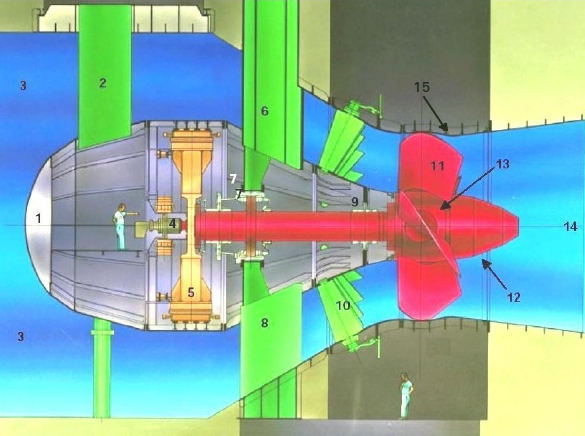
\includegraphics[width=\columnwidth]{sota/figs/intro/bulb_turbine2}
	\caption{Ilustração de uma turbina do tipo bulbo.}
	\label{fig::bulb_turbine}
\end{figure}

\begin{center}
\begin{tabular}{  c | c  }
  \hline
  \textbf{Número} & \textbf{Componente} \\ \hline
  1 & Nariz do bulbo \\ \hline
  2 & Tubo de acesso ao gerador  \\ \hline
  3 & Câmara de adução  \\ \hline
  4 & Cabeçote Kaplan  \\ \hline
  5 & Gerador Síncrono  \\ \hline
  6 e 8 & Estrutura de sustentação \\ \hline
  6 & Tubo de acesso à turbina \\ \hline
  7 e 9 & Mancais Combinado e Guia \\ \hline
  10 & Distribuidor \\ \hline
  11 & Pás do Rotor \\ \hline
  12 & Cone ou Ogiva \\ \hline
  13 & Cubo \\ \hline
  14 & Tubo de sucção/descarga \\ \hline
  15 & Aro Câmara \\
  \hline
\end{tabular}
\captionof{table}{Componentes principais de uma turbina tipo bulbo}
%\caption{Componentes principais de uma turbina tipo bulbo}
\label{tab::bulb_turbine}
\end{center}



Atualmente, caso seja necessário algum reparo ou inspeção na turbina, é necessário que se interrompa o fluxo de água e que 
toda a água em seu interior seja drenada. Para manutenção do rotor, existe uma escotilha de acesso de diâmetro limitado. Entretanto, caso deseje-se realizar 
a metalização de pás já instaladas, utilizando-se os processos atuais, é
necessária a retirada de todo o aro câmara, desmontagem completa do rotor e logística de transporte das pás até o local
onde a metalização será realizada. Essa operação, caso necessite ser realizada, demandaria a mobilização
de diversas equipes de manutenção, operação de pórtico rolante e transporte,
além de impossibilitar a utilização da turbina durante várias semanas.
No contexto da solução proposta, os pontos de interesse da turbina são:

\begin{itemize}
  \item Hélice e pás;
  \item Aro Câmara e regiões adjacentes;
  \item Escotilhas de acesso;
  \item Tubo de Sucção;
  \item Infraestrutura disponível
\end{itemize} 

\subsubsection{Hélice e pás}
 
O rotor ou hélice da turbina é constituído do cubo, as pás e o cone. 
Nas turbinas da usina Jirau, cada pá mede, aproximadamente, 2,5m de altura e
3m de largura. A partir do interior da turbina, todas as superfícies da pá são
alcançáveis, com exceção da borda e do lip da pá. O único ponto de acesso à
essa regiâo é por meio da escotilha superior de acesso. A figura
\ref{fig::blade_rijeza} exemplifica uma pá do rotor presente na usina Jirau recém metalizada no galpão da Rijeza.

\begin{figure}[h!]
	\centering	
	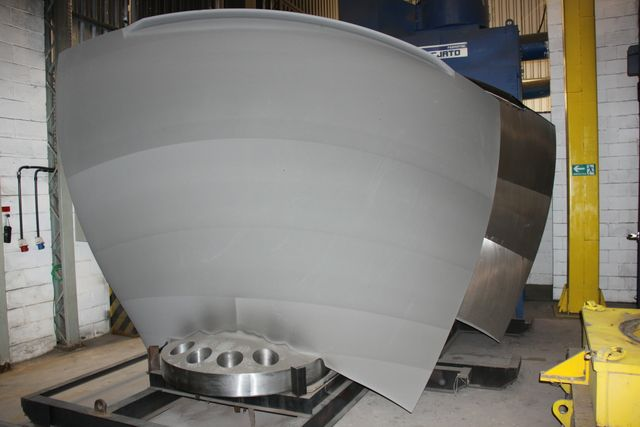
\includegraphics[width=0.7\columnwidth]{sota/figs/viagem/img_4887}
	\caption{Pá do rotor recém metalizada.}
	\label{fig::blade_rijeza}
\end{figure}

A angulação de cada pá em relação ao fluxo d'água pode ser alterado em 29$^o$,
14.5$^o$ para cada lado a partir da posição inicial, não havendo sobreposição
entre as pás, como ilustrado na figura \ref{fig::blades_angle}.
Essa angulação pode ser explorada para otimizar o espaço de trabalho necessário
para o processamento da pá e também influencia o acesso à região
entre o distribuidor e o rotor, uma vez que não existe acesso pela montante da
turbina. Entretanto, vale observar que esta angulação não pode ser alterada
manualmente e só pode ser realizada uma vez, antes do desligamento da turbina. A
posição do rotor também pode ser manualmente alterada, possibilitando que o mesmo seja girado em ambas as direções e sem limite de revoluções. Entretanto, essa operação é uma tarefa imprecisa e envolve um certo risco às pessoas que a realizam. Sendo
assim, a solução proposta deve otimizar o número de rotações necessárias para o processamento de todas as pás.

\begin{figure}[h!]	
	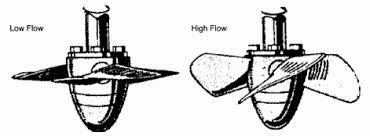
\includegraphics[width=\columnwidth]{sota/figs/intro/blades_angle}
	\caption{Exemplo de limites de rotação das pás do rotor.}
	\label{fig::blades_angle}
\end{figure}

\subsubsection{Aro Câmara e regiões adjacentes}

O aro câmara, assim como o a região próxima ao distribuidor e também ao tubo de
sucção possuem superfícies metálicas. Essa característica possibilita a
exploração de soluções de fixação magnética.

Somente a região compreendida pelo aro câmara é plana e tendo como agravante a presença do distribuidor na região à 
montante ao rotor. É necessário que a inclinação presente nessas superfícies seja contabilizada e uma solução eficiente 
de apoio ou plano elevado seja desenvolvida caso haja necessidade de fixação de alguma parte do sistema. Atualmente todo 
o trabalho é realizado por meio da montagem de andaimes ancorados por cordas. %A
%figura \ref{fig::andaime} ilustra uma estrutura utilizada no modo de inspeção e
%manutenção atuais.

%\begin{figure}[h!]	
%	\centering
%	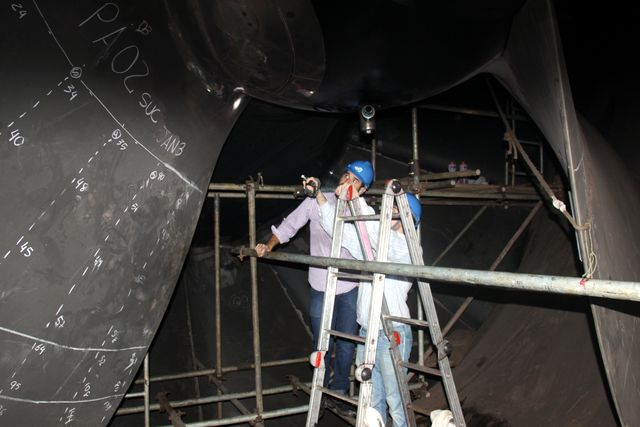
\includegraphics[width=0.8\columnwidth]{sota/figs/viagem/img_4969}
%	\caption{Andaime montado no interior da turbina e ancorado por cordas}
%	\label{fig::andaime}
%\end{figure}

 
\subsubsection{Escotilhas de acesso}
O acesso à turbina se dá por duas escotilhas, uma inferior, localizada no ínicio do tubo de sucção 
próxima ao aro câmara e outra superior, localizada na parte superior do aro câmara.

A escotilha inferior, ilustrada na figura \ref{fig::esc_inf} é o acesso
utilizado para a entrada de pessoas na turbina e todo material utilizado para reparos é transportado através dessa escotilha. Na usina Jirau existem dois 
tipos de escotilha de acesso inferior, sendo a menor delas possuindo 80cm de diâmetro. 

A escotilha superior é utilizada, principalmente, para a inspeção visual do
estado dos Lips das pás.
O diâmetro do acesso superior é de aproximadamente $35.7cm$, limitando as
dimensões dos equipamentos que podem ser transportados através da escotilha. As figuras \ref{fig::esc_sup_ext} e
\ref{fig::esc_sup_int} ilustram o acesso à escotilha superior pelo exterior ao
aro câmara e a visão pelo interior da turbina,
respectivamente.

\begin{figure}[h!]	
	\centering
	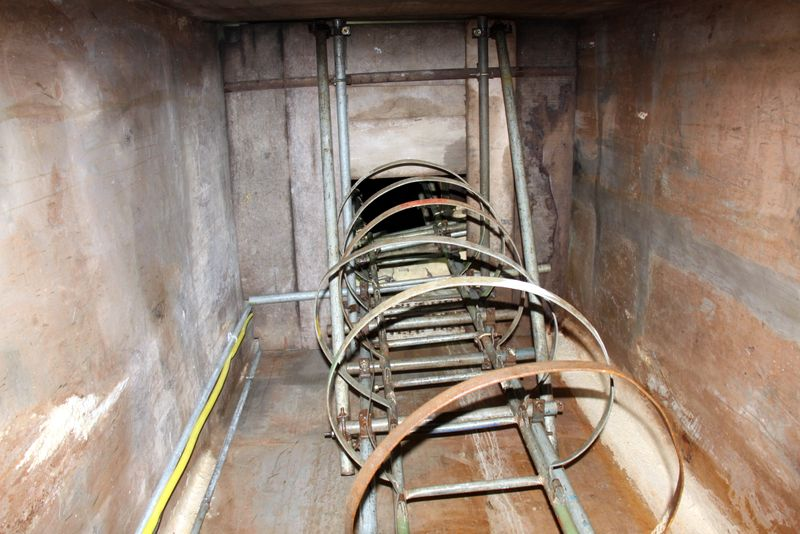
\includegraphics[width=0.8\columnwidth]{figs/esc_inf}
	\caption{Vista exterior da escotilha inferior.}
	\label{fig::esc_inf}
\end{figure}




\begin{figure}[h!]	
	\centering
	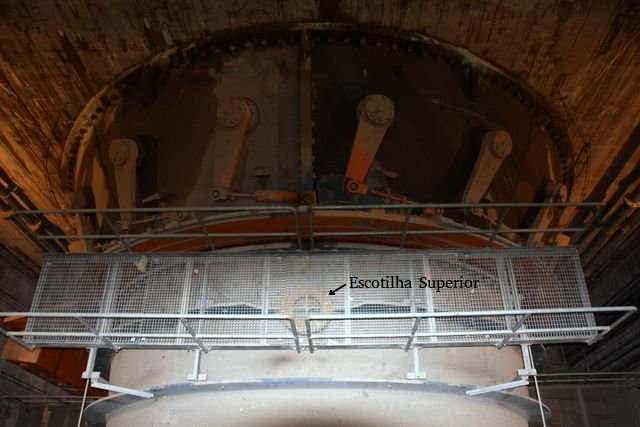
\includegraphics[width=0.8\columnwidth]{sota/figs/viagem/img_4979_mod}
	\caption{Vista da escotilha superior pelo exterior do aro câmara}
	\label{fig::esc_sup_ext}
\end{figure}

\begin{figure}[h!]	
	\centering
	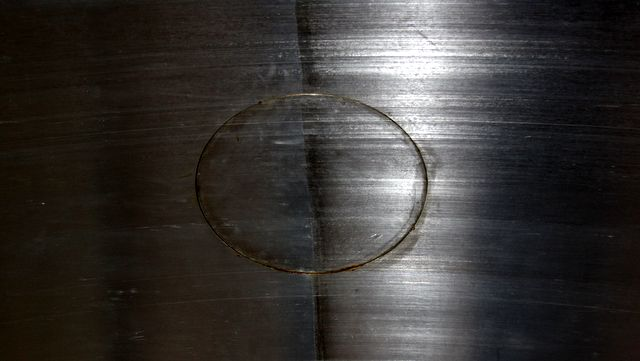
\includegraphics[width=0.8\columnwidth]{sota/figs/viagem/img_4982}
	\caption{Vista da escotilha superior pelo interior do aro câmara}
	\label{fig::esc_sup_int}
\end{figure}

\subsubsection{Tubo de sucção}

Ao final do tubo de descarga está localizado o vão dos stoplogs 
de jusante ou da comporta vagão e, em seguida, o leito do rio, como ilustrado
na figura \ref{fig::tubo_suc}.
Caso os stoplogs não estejam inseridos, existe um vão de, pelo menos, 10 m de largura. Porém, não
é válida a utilização deste vão como acesso à turbina, pois há grande fluxo de
água devido à abertura do distribuidor. O distribuidor não é fechado
imediatamente por questões ambientais, já que este é o escoamento de peixes.

%criando assim
%um acesso extra para um sistema submarino. A figura \ref{fig::tubo_suc}
%exemplifica a magnitude do tamanho do acesso, deixando claro que o limitante de
%tamanho do sistema para a utilização desse acesso é o vão de entrada do
% stoplog, ilustrado na figura \ref{fig::stoplog}. Outra alternativa é utilizar um
%guindaste e submergir o sistema pelo próprio rio, entretanto o sistema ficaria
%sujeito as condições do ambiente.

\begin{figure}[H]
	\centering	
	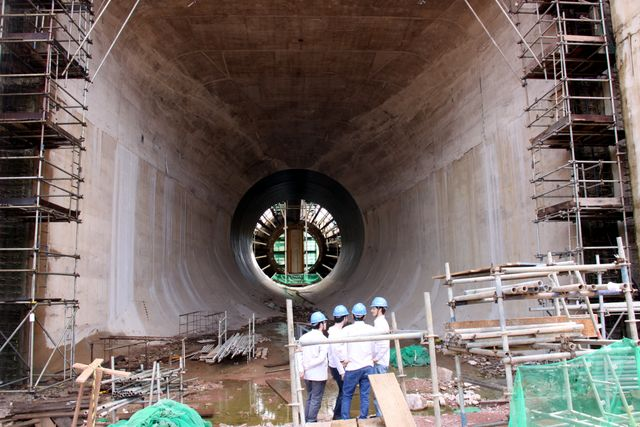
\includegraphics[width=0.8\columnwidth]{sota/figs/viagem/img_5086}
	\caption{Abertura do tubo de sucção para o leito do rio, em fase de
	construção.}
	\label{fig::tubo_suc}
\end{figure}

\subsubsection{Infraestrutura disponível}
É importante ressaltar a infraestrutura dísponível para o desenvolvimento da solução. 
Após o ensecamento da turbina, é possível a disponibilização de energia elétrica
e ar comprimo em seu interior, ambos importantes para o processo de metalização. Outro fator 
importante é a presença de um pórtico rolante que tem acesso até o andar diretamente 
inferior ao aro câmara, posicionando todo o equipamento necessário nas proximidades 
da escotilha de acesso inferior. É possível também o acesso direto, por meio de pórtico, 
à escotilha superior.

\begin{figure}[h!]	
	\centering
	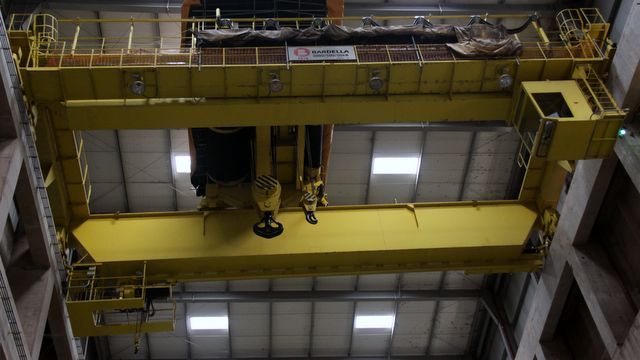
\includegraphics[width=0.8\columnwidth]{sota/figs/viagem/img_4989}
	\caption{Pórtico rolante com acesso ao exterior do aro câmara}
	\label{fig::portico}
\end{figure}


O ambiente pode ser resumidamente caracterizado pelas dimensões das pás,
elemento a ser processado; características do aro câmara, estrutura que limita o
espaço de trabalho do robô; e pelos acessos nos quais o sistema terá que
utilizar:

\begin{itemize}
  \item \textbf{Pás do rotor} - Material aço inox 420. Dimensões 2.5 x 2.5 m de superfície;
  \item \textbf{Aro Câmara} - estrutura cilíndrica com raio de 3.95 m e
  superfície metálica;
  \item \textbf{Acessos}: 
  	\begin{itemize}
    	\item Escotilha superior - 35 cm de diâmetro;
  		\item Escotilha inferior - 80 cm de diâmetro;
  		\item Tubo de descarga - 20 x 20 m, porém acessado pelo rio. 
  	\end{itemize}
\end{itemize}







\subsection{Descrição das tarefas do robô}
\label{desc_taref}
Esta subseção descreve as tarefas básicas do robô para o revestimento de
turbinas \textit{in situ}. Em linhas gerais, o robô a ser desenvolvido deve ser
capaz de realizar a tarefa de revestimento tal qual seria feita caso a pá não estivesse instalada na
tubina e de uma maneira autônoma. A pá, antes de ser submetida ao
processo de revestimento, deve estar em conformidade com o gabarito, perfil hidráulico de uma pá
intacta. Portanto, uma tarefa do robô é realizar o mapeamento do perfil
hidráulico, construir um modelo 3D e analisar imperfeições.

Em caso de deformações, causados por cavitação e abrasão, estas precisam
ser removidas manualmente ou de forma automatizada, possivelmente por
soldagem. A tarefa de soldagem pode
ser realizada por operador, manualmente, por não possuir todas as restrições
da tarefa de revestimento (velocidade, precisão, carga e etc), porém o ambiente
pode dificultar a operação de forma que a execução por um robô seja
indispensável. 

Após as pás estarem de acordo com o gabarito, faz-se a
identificação do desgaste do revestimento, medindo sua espessura em pontos
pontos específicos sobre a superfície da pá. Manualmente esse
processo é realizado eficientemente em 10 min, justificando a não necessidade de
esta ser uma tarefa do robô. 

Em caso de necessidade de aplicação
de novo revestimento, é necessária a remoção do revestimento antigo por
jateamento, a fim de deixar a superfície rugosa e aumentar sua aderência. A
tarefa de jateamento é atualmente realizada maualmente, mas também pode ser
realizada pelo robô. Como ambos os lados da pá são revestidos, o jateamento deve
ser realizado em ambos os lados. Vale ressaltar que, em teoria, pode-se aplicar revestimento por metalização sem retirar o último revestimento,
porém esse processo ainda se encontra em fase de estudos na Rijeza.
%Segue-se o exemplo de empresas de aviação, onde existe a
%prática de retirar todo o revestimento antigo antes de aplicar o novo.

Por fim, o robô deverá aplicar o revestimento como
forma de prevenir o dano causado pelos fenômenos abrasivos. O robô projetado
para fazer o revestimento precisa preencher todos os requisitos discutidos na
subseção~\ref{sec::desc_hvof} e ser adaptável ao ambiente, cujos as restrições
são discutidos na subseção~\ref{sec::desc_contex}. 

Das tarefas a serem relizadas, são destacadas as seguintes:

\textbf{Tarefas que podem ser executadas manualmente:}
\begin{itemize}
  \item Inspeção e análise de danos na pá, tanto para reparo quanto para
  revestimento;
  \item Reparo;
  \item Montagem do sistema;
  \item Jateamento da superfície;
\end{itemize}

\textbf{Tarefas que poderão ser executadas pelo robô:}
\begin{itemize}
  \item Modelar o perfil hidráulico;
  \item Calibração;
  \item Jateamento;
  \item Reparo (soldagem e esmerilhamento);
  \item Revestimento por metalização;
\end{itemize}




\section{Estudo de viabilidade técnica detalhada}\label{sec::viatec} 
% Author: Renan

O estudo de viabilidade técnica detalhada é realizado para cada acesso à turbina
(superior e inferior), como no capítulo  \ref{cap::sota}. O estudo passa pelas
seguintes etapas: 1) pesquisa de mercado; 2) geometria plana e/ou espacial; 3)
espaço de trabalho e cinemática do manipulador; 4) detalhamento de
bases mecânicas; 5) dinâmica do manipulador; 6) sensores para calibração; 7)
planejamento de trajetórias; e 8) técnicas de calibração.
Neste documento, serão abordadas as etapas: 1, 2, 3, 4, 5 e 6.

A pesquisa de mercado é uma busca abrangente de soluções comerciais dentro do
escopo da solução conceitual desenvolvida no capítulo \ref{cap::sota}. A
pesquisa envolve manipuladores comerciais que preencham os requisitos do processo de HVOF e
estejam de acordo com as restrições impostas pelo ambiente e o acesso. Desssa
forma, diversos fabricantes de manipuladores, Motoman, Kuka, ABB, Fanuc,
Adept e Kinova, foram avaliados e suas principais características como carga,
peso, dimensões, velocidade, temperatura e umidade de operação, são analisadas.
A pesquisa de mercado tem como objetivo retornar o objeto para os outros
estudos, ou seja, o manipulador a ser utilizado na solução.

O estudo puramente geométrico, apesar de ser diferente para cada acesso, é
genericamente uma abordagem simplificada e analítica do problema e desconsidera
alguns fatores do ambiente. O estudo geométrico tem como objetivo retornar um caso
aproximado da situação real e estimar as possíveis soluções da posição do
manipulador em relação à pá, de forma que toda ela seja revestida.

O espaço de trabalho e cinemática do manipulador é uma abordagem
detalhada e de simulação. Ela considera: o meio estruturado, em um ambiente de
simulação; o manipulador com suas dimensões e limites de juntas reais;
possibilidade de colisões; real espaço de trabalho do manipulador; modelos de
bases para o manipulador; e possiveis sensores. Para a simulação é utilizada a
plataforma Openrave, uma arquitetura de planejamento para robôs autônomos,
sendo possivelmente integrada para controle em tempo real e monitoramento.
Ela provê funcionalidades para operações de cinemática direta e inversa, e
simulações físicas, e apresenta ferramentas e interfaces para planejamento de
manipuladores e um protocolo que interpreta scripts na linguagem MatLab, Octave
e Python \citep{diankov2008openrave}.

Na seção de estudo da dinâmica de manipuladores robóticos, serão realizadas
análises numéricas e analíticas, em um ambiente de simulação, de cinemática
diferencial e torques das juntas de manipuladores, utilizando as características
do processo de revestimento. O estudo tem por objetivo tornar a simulação mais
realista, analisar a execução do processo para algumas distâncias da pá
e verificar a manipulabilidade do robô.

A base mecânica é definida como a estrutura de suporte e transporte do robô.
Esta deve permitir ao manipulador alcançar os posicionamentos necessários, 
definidos nos estudos cinemáticos e dinâmicos. Para que estes
posicionamentos sejam alcançados, a base mecânica oferece graus de
liberdade ao sistema base e robô, adequados para levar a base do robô aos pontos
ótimos para o revestimento de uma região da pá. Como principais diretrizes para
o projeto da base mecânica, são considerados: a resistência aos esforços dinâmicos do
manipulador; baixas vibrações; modularidade; e facilidade de transporte,
montagem e ajuste. O estudo dos conceitos analisados para a base mecânica serão
demonstrados em detalhe na seção~\ref{sec::base_mec}.

As características e desafios logísticos da escotilha inferior já foram
previamente apresentados no capítulo \ref{cap::sota}, sendo aqui apontadas, na
tabela~\ref{tab::bighatch}, apenas as suas principais caracterísiticas para o
desenvolvimento de uma solução detalhada.

\begin{center}
\begin{tabular}{  c | c  }
  \hline
  \textbf{Informação} & \textbf{Dado} \\ \hline
  Dimensões do acesso & 800 mm de diâmetro  \\ \hline
  Distância do acesso à pá & 4000 mm  \\ \hline
  Distância do solo & 5000 mm \\ \hline
  Peso máximo manipulável & 150 Kg \\
  \hline
\end{tabular}
\captionof{table}{Dados principais da escotilha inferior}
%\caption{Dados principais do processo de metalização HVOF}
\label{tab::bighatch}
\end{center}

\subsection{Pesquisa de mercado}
% Author: Renan
A pesquisa de mercado está detalhadamente explicada na
tabela~\ref{ape::bighatch}, no apêndice. Os seguintes robôs satisfazem os
requerimentos e restrições principais, de acordo com as tabelas~\ref{tab::bighatch} e ~\ref{tab::hvof}, e os requisitos abordados
em \ref{sec::desc_contex}: Viper s1300 (Adept), ARC Mate 100iC/12 (Fanuc),
M-10iA/12S (Fanuc), LBR iiwa 14 R820 (Kuka), KR 10 R1100 sixx WP (Kuka), MH6F-10
(Motoman), SIA10F (Motoman), MH12 (Motoman), SIA20D (Motoman). Destes, os
manipuladores LBR iiwa 14 R820 (Kuka) e Viper s1300 (Adept) deverão passar por adaptações para
operar em temperaturas até $40^o$C e umidade relativa no ar de $91\%$; e os
manipuladores KR 10 R1100 sixx WP (Kuka), MH6F-10
(Motoman) e SIA10F (Motoman) têm carga máxima de 10 Kg, que é o limite para o
processo. Dessa forma, os manipuladores comerciais prontos para o uso e que
trabalha com folga em carga são: ARC Mate 100iC/12 (Fanuc), M-10iA/12S (Fanuc),
MH12 (Motoman) e SIA20D (Motoman).

Apesar de o manipulador LBR iiwa 14 R820 (Kuka) necessitar de adaptações, seu
peso (29 Kg) representa grande vantagem perante os outros manipuladores, logo
não deve ser descartado em futuros estudos. O mesmo se pode dizer do KR 10 R1100
sixx WP (Kuka), que possui 56 Kg, mas estará operando perto de sua carga limite
(10 Kg).

Os objetos de estudo são, portanto: KR 10 R1100
sixx WP (Kuka), MH12 (Motoman), LBR iiwa 14 R820 (Kuka), ARC Mate 100iC/12
(Fanuc) e SIA20D (Motoman).


 
\subsection{Estudo puramente geométrico}
% Author: Renan
A abordagem puramente geométrica é uma análise do espaço de trabalho do
manipulador na pá. Utiliza os manipuladores da pesquisa de mercado como
objetos deste estudo e leva em consideração as dimensões da
pistola, o ângulo máximo e mínimo para o revestimento ($90^o \pm 60^o$), e a
distância mínima de 230 mm entre a pistola e a pá. É um estudo simplificado por não considerar as possíveis colisões com o ambiente, assumir
que a pá está contida em um plano (projeção, objeto 2D) e considerar o espaço
de trabalho do manipulador simétrico. A abordagem geométrica foi desenvolvida
com o auxílio do software Geogebra.

Primeiramente, o espaço de trabalho do manipulador é aproximado
como uma esfera, delimitada pelo espaço de
trabalho real do manipulador. A pá é projetada em planos, como mostra a
figura~\ref{fig::paplanos}, e, conforme o manipulador se aproxima da pá, o plano
direito corta a esfera (espaço de trabalho do manipulador), FIGURA. A interseção
entre o plano e a esfera é um círculo de raio $\overline{CB^i}$, que pode ser
calculado e estimado como a área revestida da pá. A distância ótima entre o
manipulador e a pá é calculada no limite em que o ângulo
$\overline{OB^iC}=30^o$. Finalmente, podem ser calculadas quantas posições
distintas o manipulador deve assumir para que toda a pá seja revestida, a partir
do modelo planar da pá e da turbina, figura~\ref{fig::pa2D}.

Essa abordagem é específica para cada manipulador da pesquisa de mercado.

\begin{figure}[h!]
	\centering	
	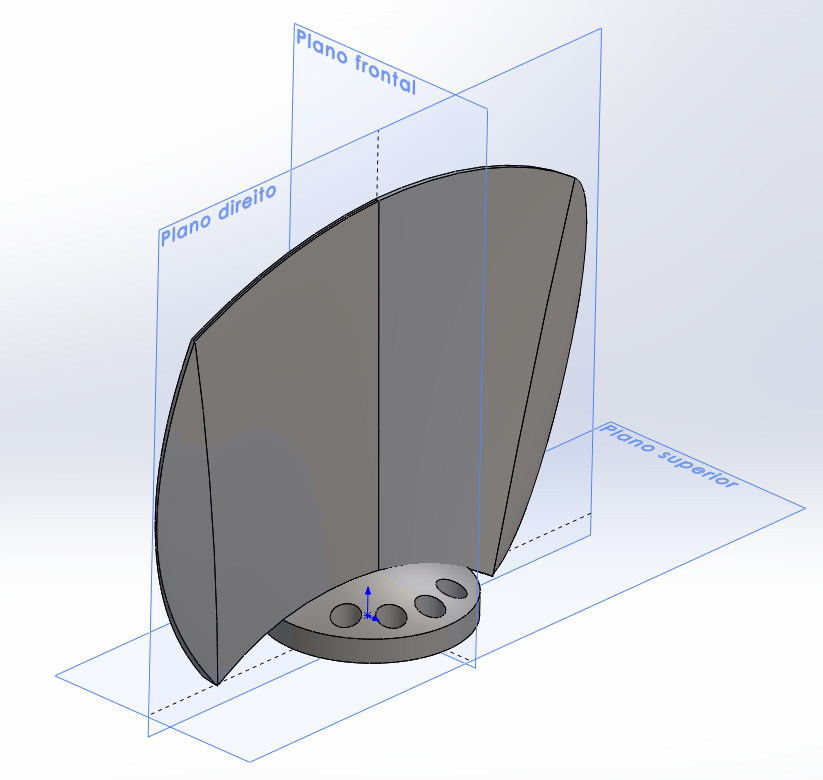
\includegraphics[width=0.6\columnwidth]{detail/figs/bighatch/PaPlanos.PNG}
	\caption{Ilustração das projeções da pá em planos.}
	\label{fig::paplanos}
\end{figure}

\begin{figure}[h!]
	\centering	
	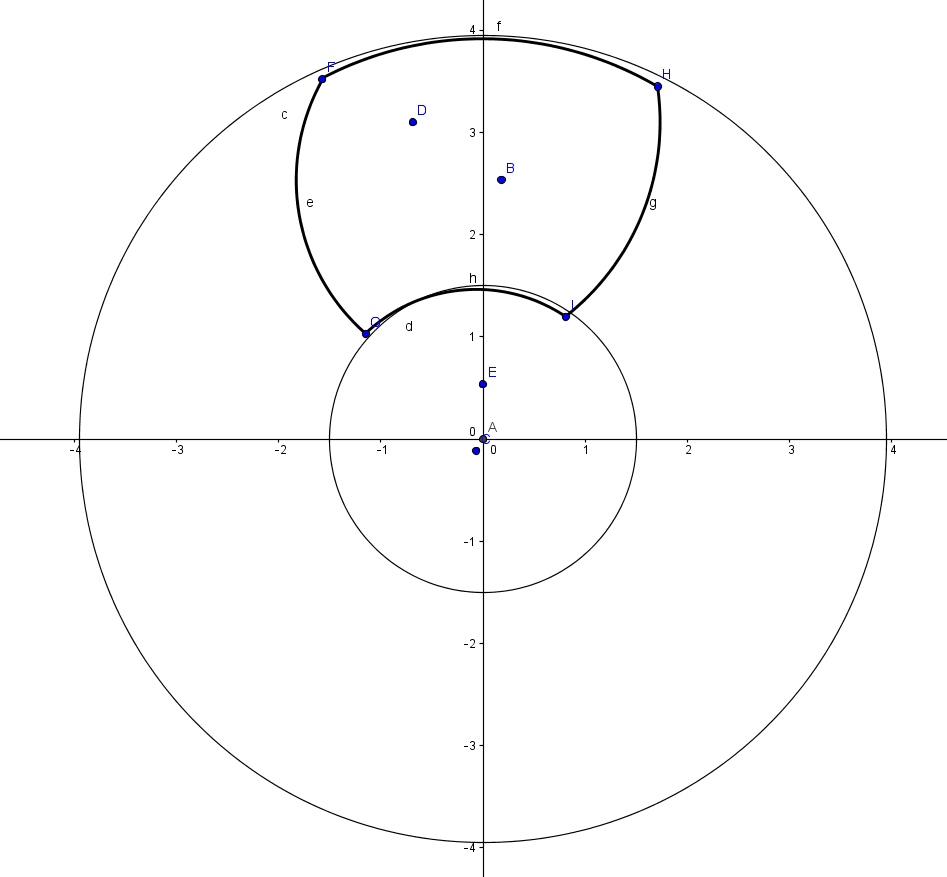
\includegraphics[width=0.6\columnwidth]{detail/figs/bighatch/pa2D.png}
	\caption{Ilustração do modelo 2D da pá.}
	\label{fig::pa2D}
\end{figure}

\paragraph{KR 10 R1100 sixx WP (Kuka)}
A figura~\ref{fig::kukageom} ilustra a interseção do espaço de trabalho
simplificado do manipulador Kuka KR10 e a projeção da pá. No
caso do Kuka KR 10 R1100, o raio da esfera é aproximado a $\overline{OB^i} = $
alcance do manipulador + comprimento da pistola + 230 mm. 

Para este manipulador, obtemos área revestida de $1.41^2\pi m^2$ e distância
ótima manipulador-pá de $0.82 m$. Dessa forma, são necessárias, pelo menos,
quatro posições distintas do manipulador a fim de toda a pá ser revestida. A
figura~\ref{fig::kukacircles} ilustra os pontos que o manipulador deve assumir
para revestir toda a pá. 

\begin{figure}[h!]
	\centering	
	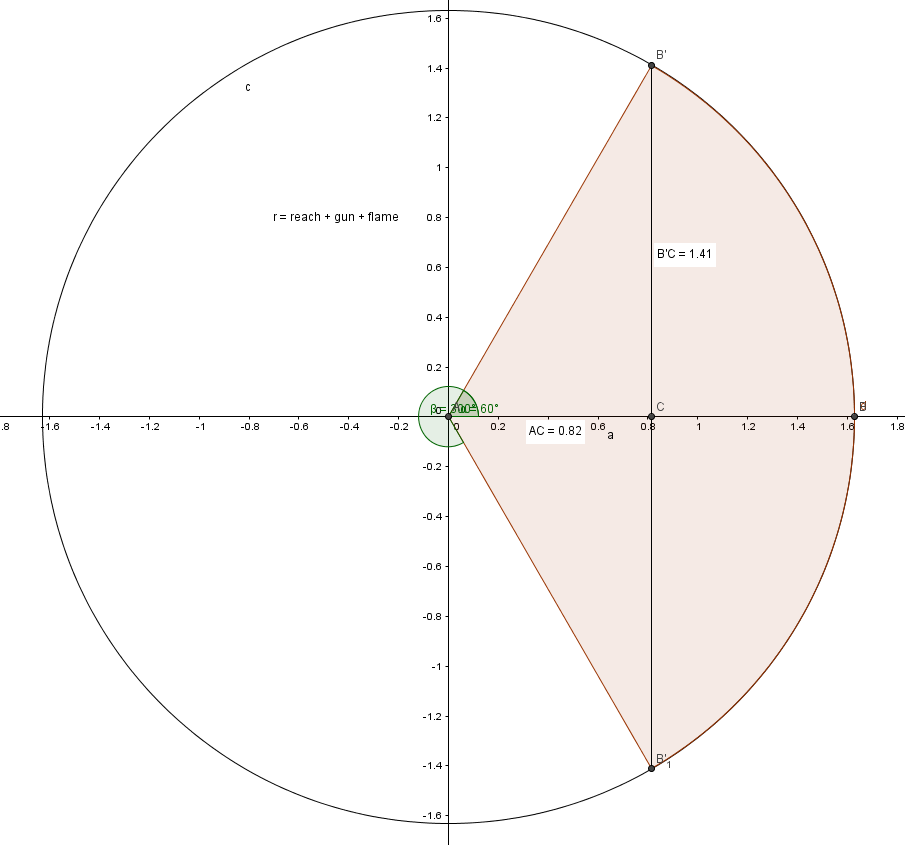
\includegraphics[width=0.6\columnwidth]{detail/figs/bighatch/kukageom.jpg}
	\caption{Ilustração da interseção do espaço de trabalho simplificado do
	manipulador Kuka KR10 e a projeção da pá.}
	\label{fig::kukageom}
\end{figure}

\begin{figure}[h!]	
	\centering
	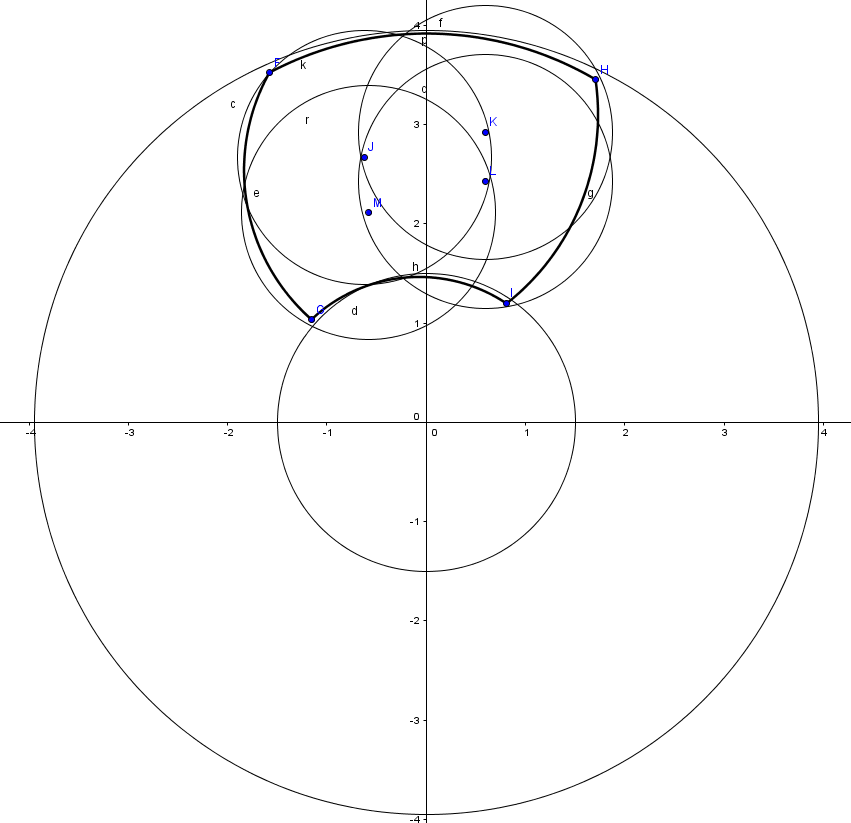
\includegraphics[width=0.6\columnwidth]{detail/figs/bighatch/kukacircles.png}
	\caption{Posições do manipulador Kuka KR10 para o processo de
	revestimento ser realizado em toda a pá.}
	\label{fig::kukacircles}
\end{figure}

\paragraph{MH12 (Motoman)}
A figura~\ref{fig::mh12geom} ilustra a interseção do espaço de trabalho
simplificado do manipulador MH12 e a projeção da pá. No
caso do MH12, o raio da esfera é aproximado a $\overline{OB^i} = $
alcance do manipulador + comprimento da pistola + 230 mm. 

Para este manipulador, obtemos área revestida de $1.54^2\pi m^2$ e distância
ótima manipulador-pá de $0.89 m$. Dessa forma, são necessárias, pelo menos,
duas posições distintas do manipulador a fim de toda a pá ser revestida. A
figura~\ref{fig::mh12circles} ilustra os pontos que o manipulador deve assumir
para revestir toda a pá.		

\begin{figure}[h!]	
	\centering
	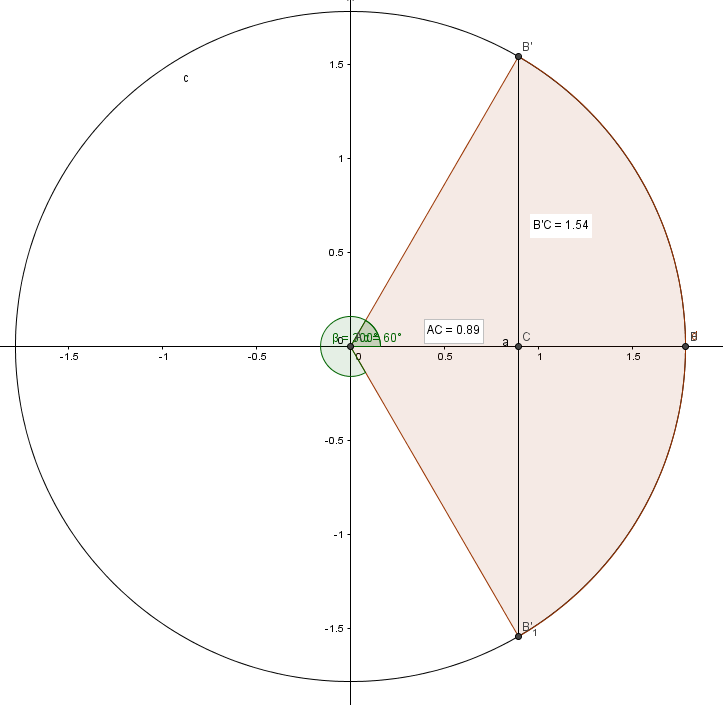
\includegraphics[width=0.6\columnwidth]{detail/figs/bighatch/mh12geom.jpg}
	\caption{Ilustração da interseção do espaço de trabalho simplificado do
	manipulador Motoman MH12 e a projeção da pá.}
	\label{fig::mh12geom}
\end{figure}

\begin{figure}[h!]	
	\centering
	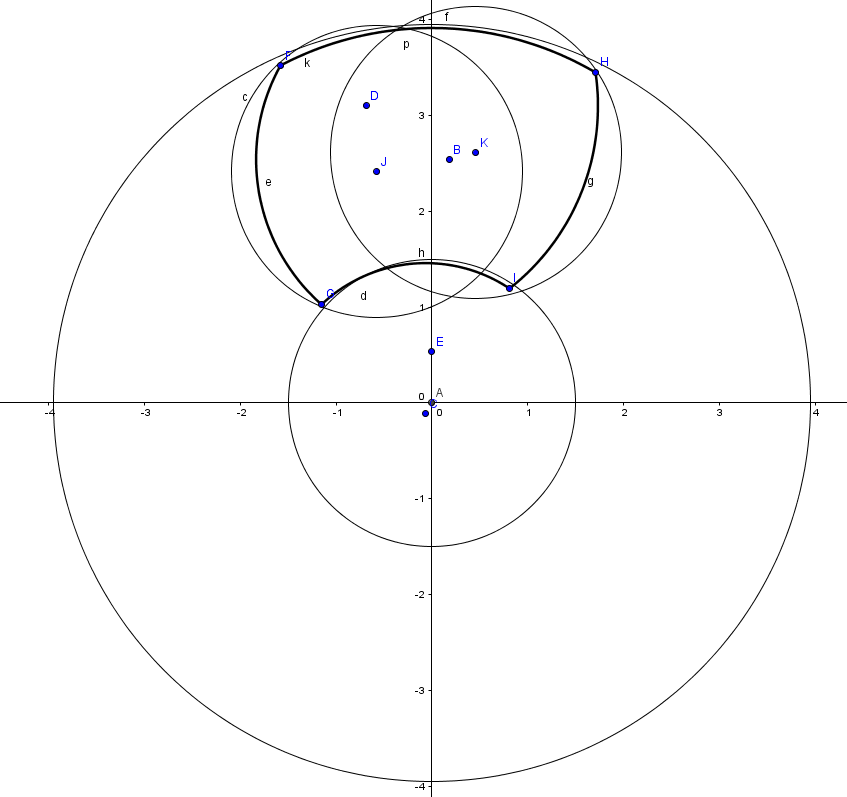
\includegraphics[width=0.6\columnwidth]{detail/figs/bighatch/mh12circles.png}
	\caption{Posições do manipulador MH12 para o processo de
	revestimento ser realizado em toda a pá.}
	\label{fig::mh12circles}
\end{figure}
\subsection{Espaço de trabalho e cinemática do
manipulador}\label{sec::cinematica} 
% Author: Renan

Como já mencionado, o ambiente de simulação
foi desenvolvido utilizando a arquitetura de planejamento Openrave. Para cada manipulador selecionado após a
pesquisa de mercado, serão analisados os reais espaços de trabalho, e o processo de
revestimento da pá em um ambiente simulado que representa as principais
caracterísiticas do ambiente real.

Para gerar o espaço de trabalho, o Openrave utiliza um método de força bruta,
onde são executadas iterações sob iterações de todas as juntas, por seus ângulos
limites e com o passo de ângulo dependendo da resolução do manipulador. O grau
de manipulabilidade do robô é representado por um gradiente de cores, cujo grau
varia do azul claro (menor manipulabilidade) ao vermelho escuro (maior manipulabilidade).
Entende-se por manipulabilidade a capacidade que o robô possui de manipular
objetos em direções específicas, isto é, para uma posição específica é
possível alcançar variadas orientações. Em todas as simulações, a pistola foi
representada como um cilindro de comprimento 300 mm e raio 50 mm, e o efetuador está no extremo do cilindro.

A superfície da pá é amostrada, formando uma grade de tamanho fixo. A técnica
\textit{axis-aligned bounding box (AABB)} é utilizada para obter os
pontos e suas respectivas normais, na superfície da pá. Nesta técnica, a
superfície alvo é inscrita em um bloco, que é uniformemente amostrado. É, então,
realizada uma verificação de colisão entre os pontos amostrados no bloco e a
superfície alvo e, caso haja interseção, o ponto é armazenado junto com sua
normal à superfície. Dessa forma, podemos amostrar a pá e deslocar estes pontos
230 mm em relação à sua normal com a superfície, garantindo a requerimento do
revestimento. A representação dos pontos amostrados e deslocados em relação às
normais da pá podem estão nas figuras~\ref{fig::amostrapa1} e ~\ref{fig::amostrapa2}. 

Utilizando as informações dos pontos amostrados e o espaço de trabalho do
manipulador, foram gerados scripts para calcular a
melhor distância do manipulador em relação a pá, de forma que o maior número de
pontos revestidos com angulação de $90^o$ fossem cobertos.
Essa distância é calculada em relação à normal da pá. Com esse dado, é possível estimar quantas posições da base do
manipulador serão necessários para o revestimento de toda a pá.

\begin{figure}[h!]	
	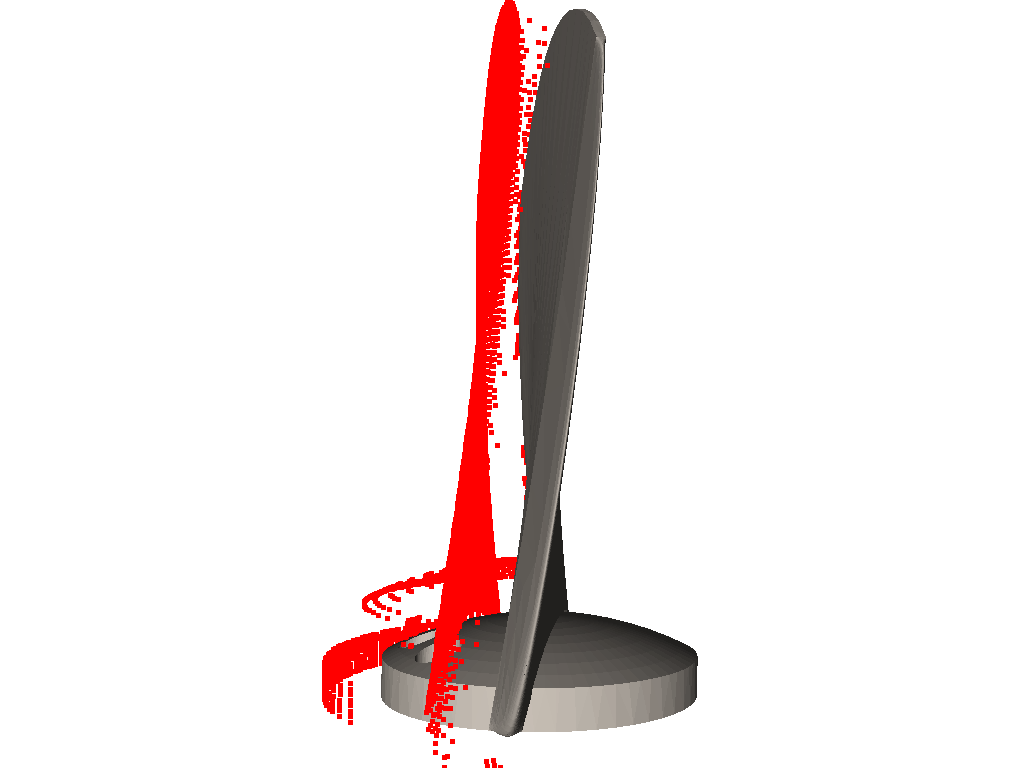
\includegraphics[width=\columnwidth]{detail/figs/bighatch/amostrapa1.png}
	\caption{Pontos amostrados da pá - vista lateral}
	\label{fig::amostrapa1}
\end{figure}

\begin{figure}[h!]	
	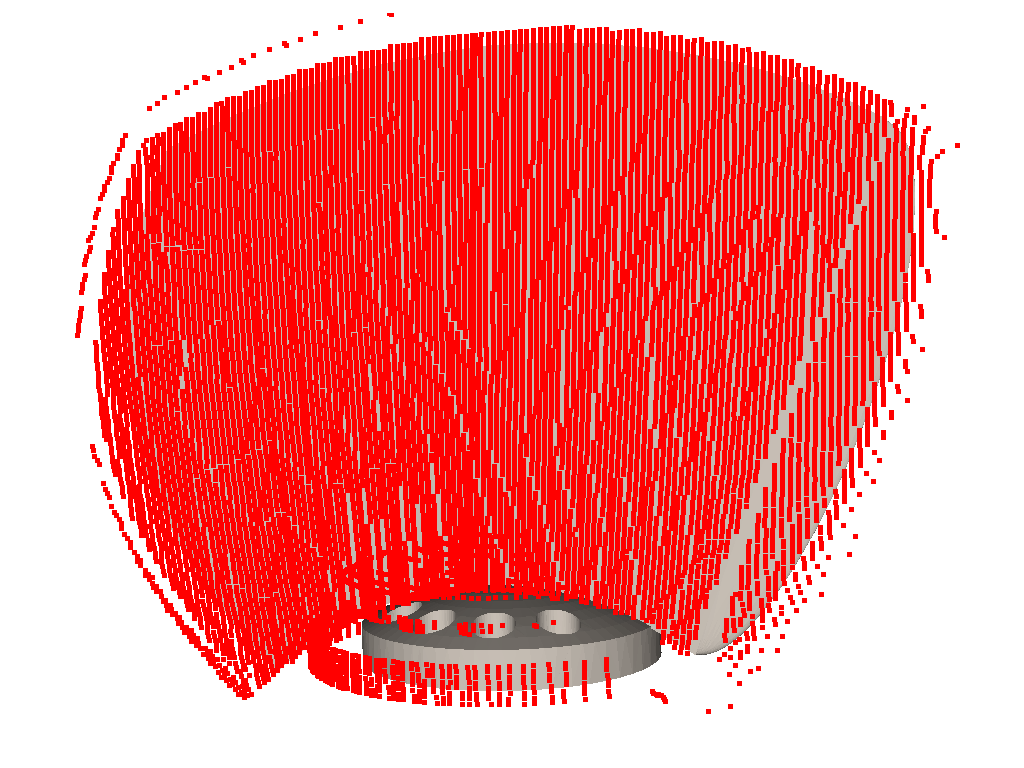
\includegraphics[width=\columnwidth]{detail/figs/bighatch/amostrapa2.png}
	\caption{Pontos amostrados da pá - vista frontal}
	\label{fig::amostrapa2}
\end{figure}

As tabelas~\ref{tab::robocarac} e ~\ref{tab::robocarac} abaixo resume as
caracterísitcas de cada robô e o estudo cinemático realizado, respectivamente:

\begin{center}
\begin{tabular}{  c | c | c | c  }
  \hline
  \textbf{Robô} & \textbf{Payload (Kg)} & \textbf{Massa (Kg)} & \textbf{Alcance
  (mm)} \\ \hline 
  KR10 & 10 & 56 & 1100 \\ \hline
  MH12 & 20 & 130 & 2551  \\ \hline
  LBR 14 & 14 & 30 & 820 \\ \hline
  SIA20D & 20 & 120 &  910 \\
  \hline
\end{tabular}
\captionof{table}{Caracterísitcas principais dos robôs.}
\label{tab::robocarac}
\end{center}

\begin{center}
\begin{tabular}{  c | c | c }
  \hline
  \textbf{Robô} & \textbf{Pontos revestidos (\%)} & \textbf{Posições de base} \\ \hline 
  KR10 & 24.33 & 13\\ \hline 
  MH12 & 53.3 & 4   \\ \hline
  LBR 14 $\uparrow$ & 17.2 & 13 \\ \hline
  LBR 14 $\rightarrow$ & 17.37 & 13 \\ \hline
  SIA20D $\uparrow$ & 23.14 & 9 \\ \hline
  SIA20D $\rightarrow$ & 24.76 & 9 \\ 
  \hline
\end{tabular}
\captionof{table}{Resumo do estudo
cinemático.}
\label{tab::robocin}
\end{center}

\paragraph{KR 10 R1100 sixx WP (Kuka)}
A figura~\ref{fig::kr10cin1} e figura~\ref{fig::kr10cin2} mostram as vistas
lateral e superior do espaço de trabalho do manipulador, respectivamente. Em
vermelho, estão representados os pontos a serem revestidos e em preto os pontos
que o manipulador foi capaz de revestir.

O script que calcula a melhor posição da base em relaçao à pá retornou a posição
870 mm, sendo que 3825 pontos foram revestidos, representando 24.33\% de toda a
pá. Estima-se que serão necessários, pelo menos, 13 posições para o recobrimento
de toda a pá, figura~\ref{fig::kr10bestpos}.



\begin{figure}[h!]	
	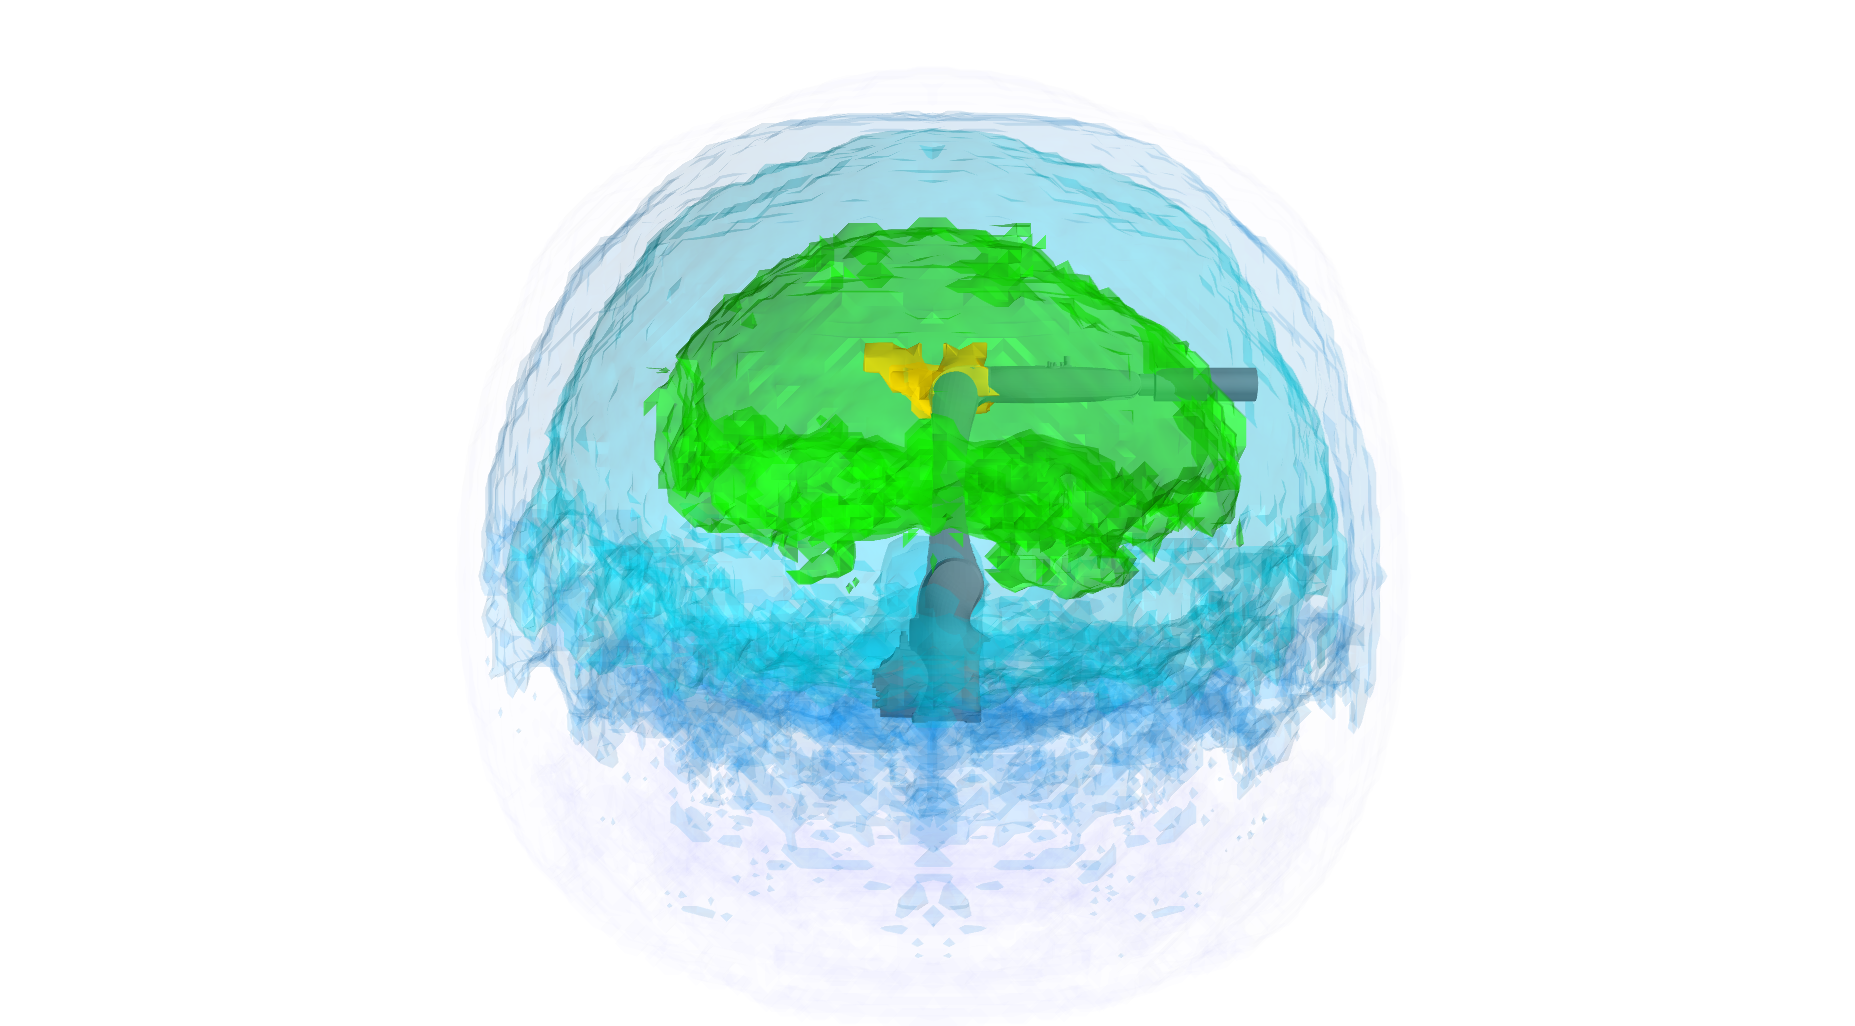
\includegraphics[width=\columnwidth]{detail/figs/bighatch/kr10_front.png}
	\caption{Espaço de trabalho do manipulador Kuka KR10 - vista lateral}
	\label{fig::kr10cin1}
\end{figure}

\begin{figure}[h!]	
	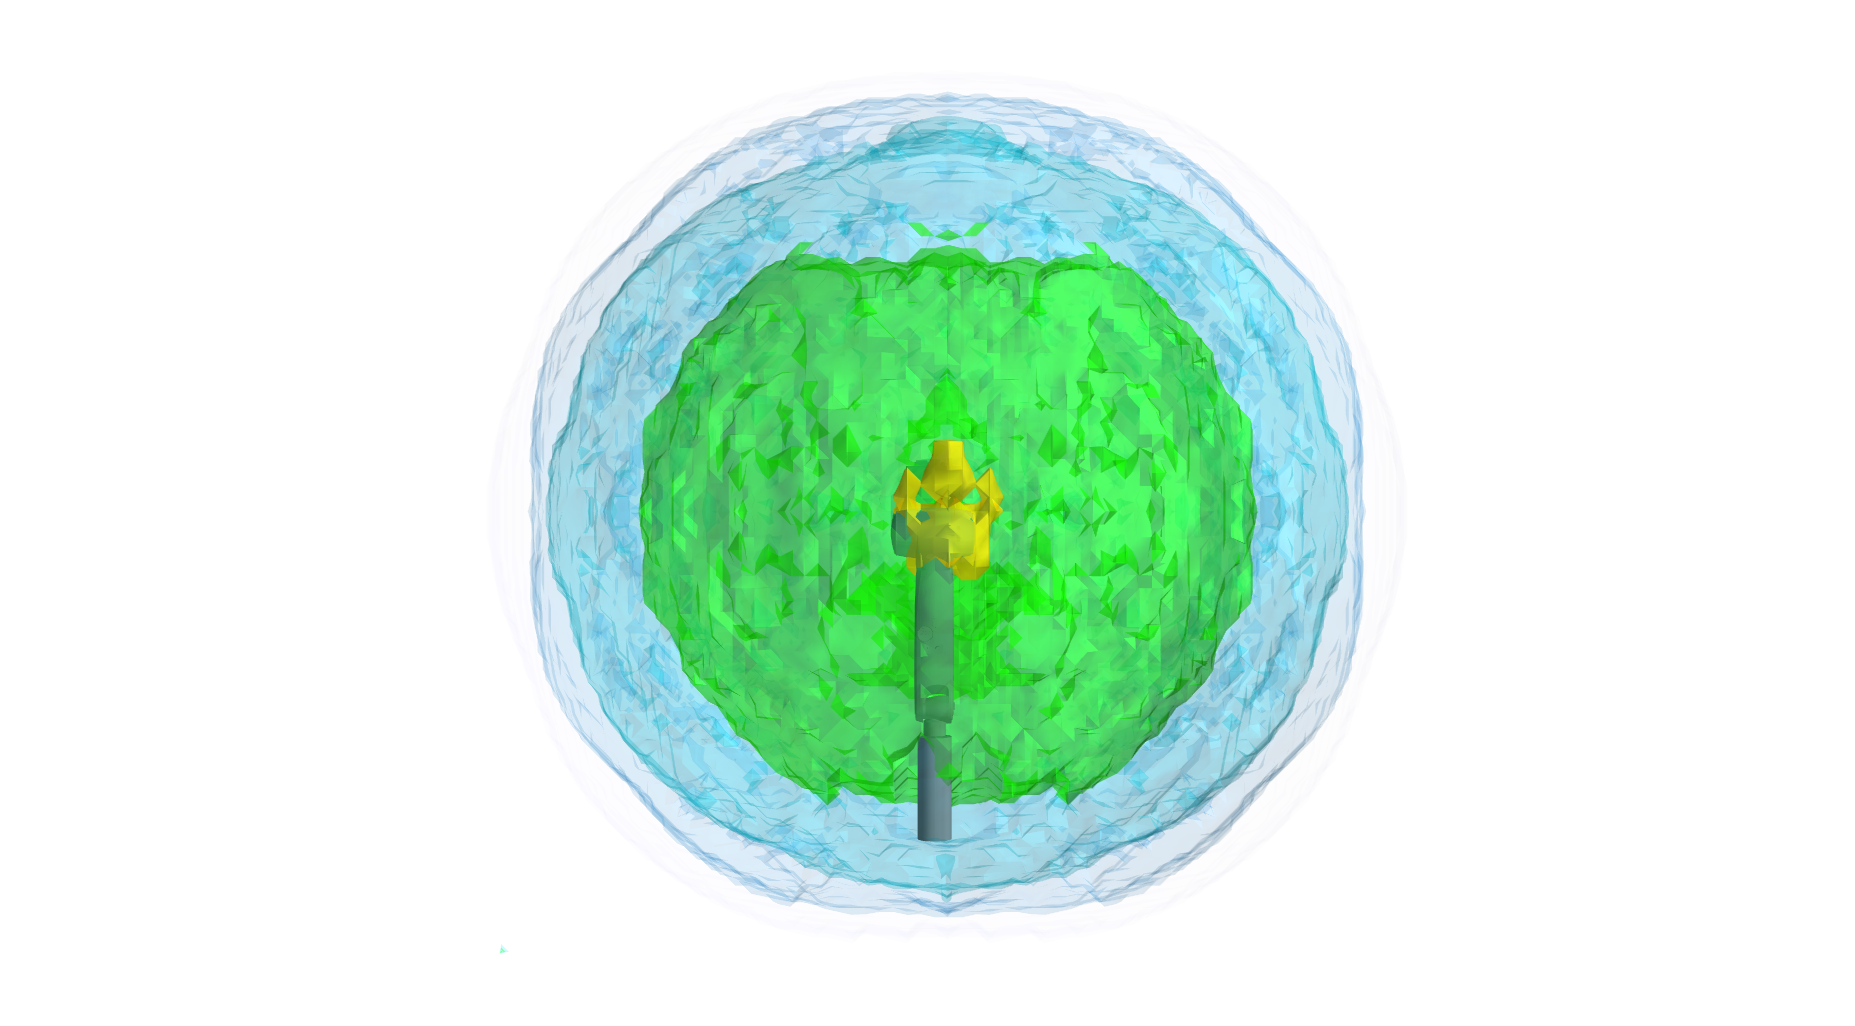
\includegraphics[width=\columnwidth]{detail/figs/bighatch/kr10_top.png}
	\caption{Espaço de trabalho do manipulador Kuka KR10 - vista superior}
	\label{fig::kr10cin2}
\end{figure}

\begin{figure}[h!]	
	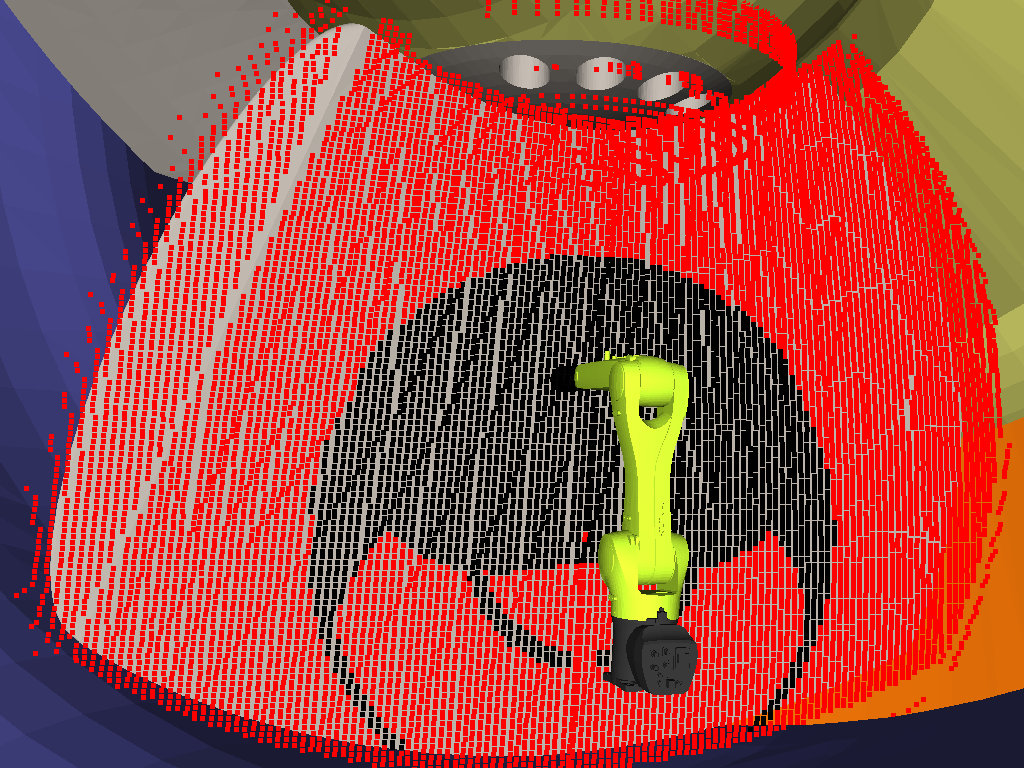
\includegraphics[width=\columnwidth]{detail/figs/bighatch/kr10_bestpos.png}
	\caption{Melhor posição para o revestimento - robô KR10 da Kuka.}
	\label{fig::kr10bestpos}
\end{figure}


\paragraph{MH12 (Motoman)}
A figura~\ref{fig::mh12cin1} e figura~\ref{fig::mh12cin2} mostram as vistas
lateral e superior do espaço de trabalho do manipulador, respectivamente.

O script que calcula a melhor posição da base em relaçao à pá retornou a posição
950 mm, sendo que 8379 pontos foram revestidos, representando 53.30\% de toda a
pá. Estima-se que serão necessários, pelo menos, 4 posições para o recobrimento
de toda a pá, figura~\ref{fig::mh12bestpos}.

\begin{figure}[h!]	
	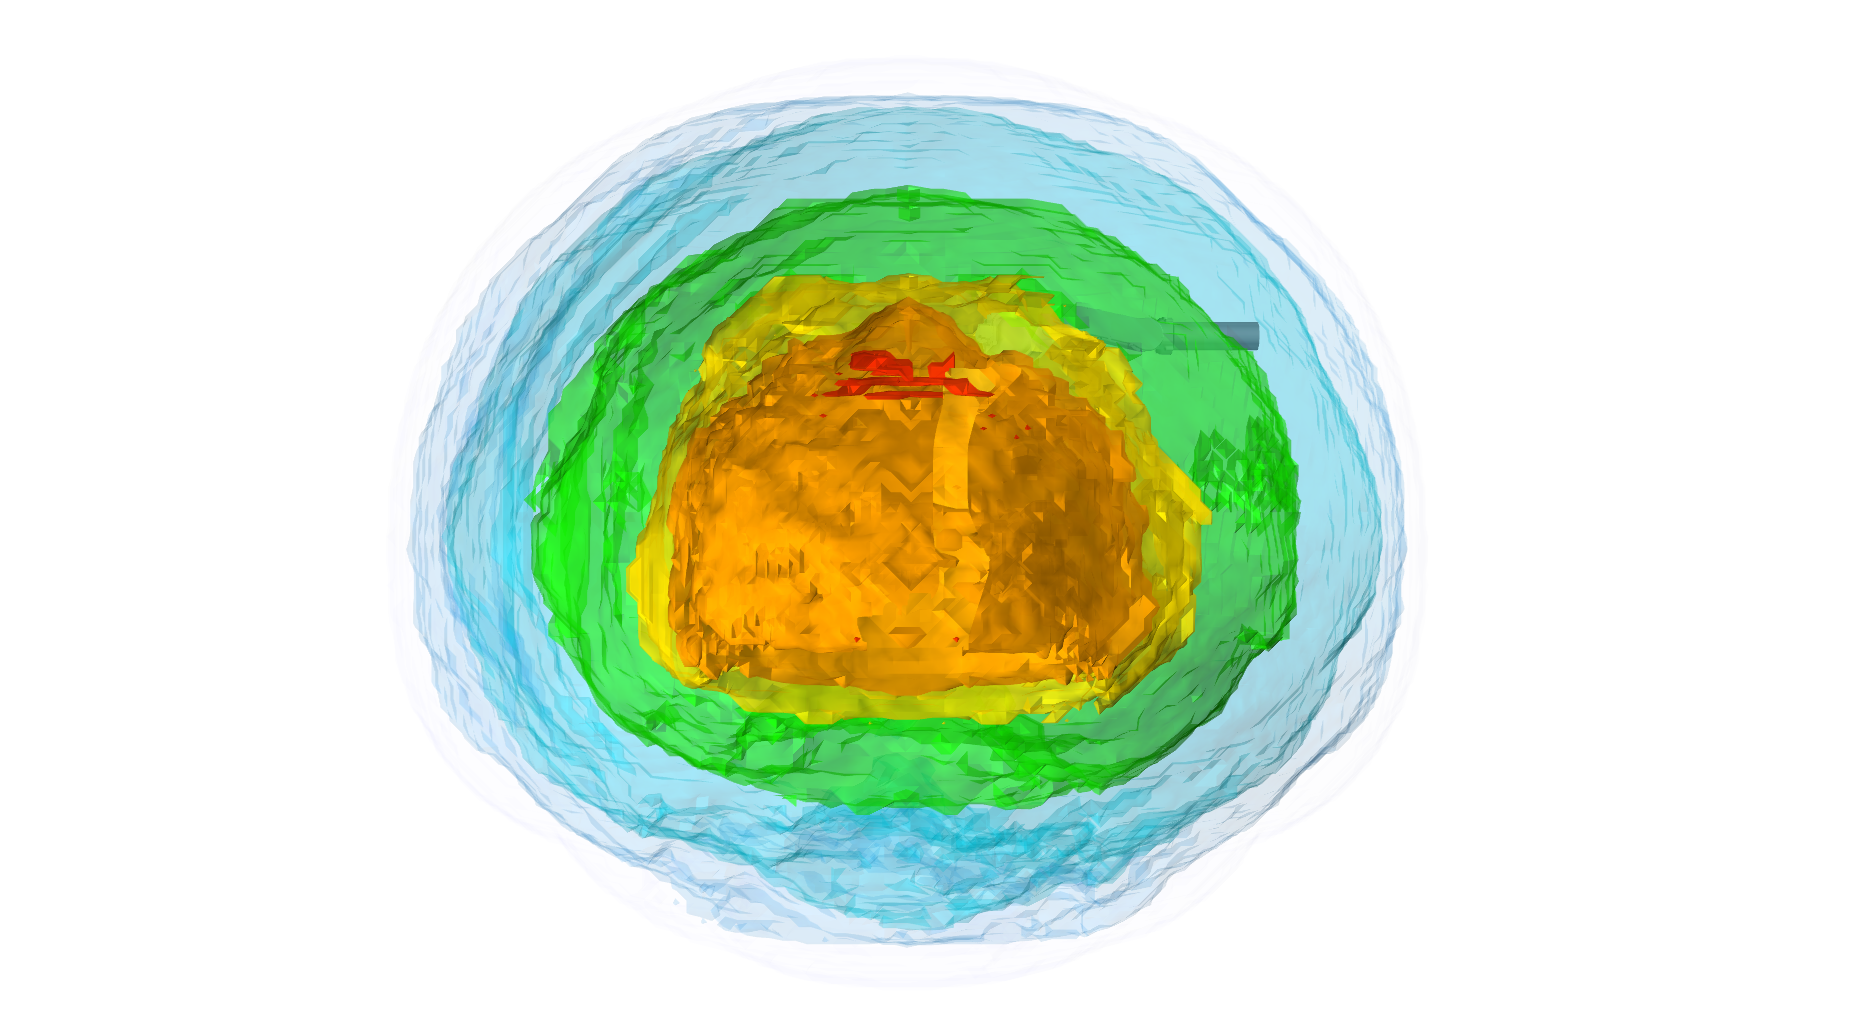
\includegraphics[width=\columnwidth]{detail/figs/bighatch/mh12_front.png}
	\caption{Espaço de trabalho do manipulador MH12 - vista lateral}
	\label{fig::mh12cin1}
\end{figure}

\begin{figure}[h!]	
	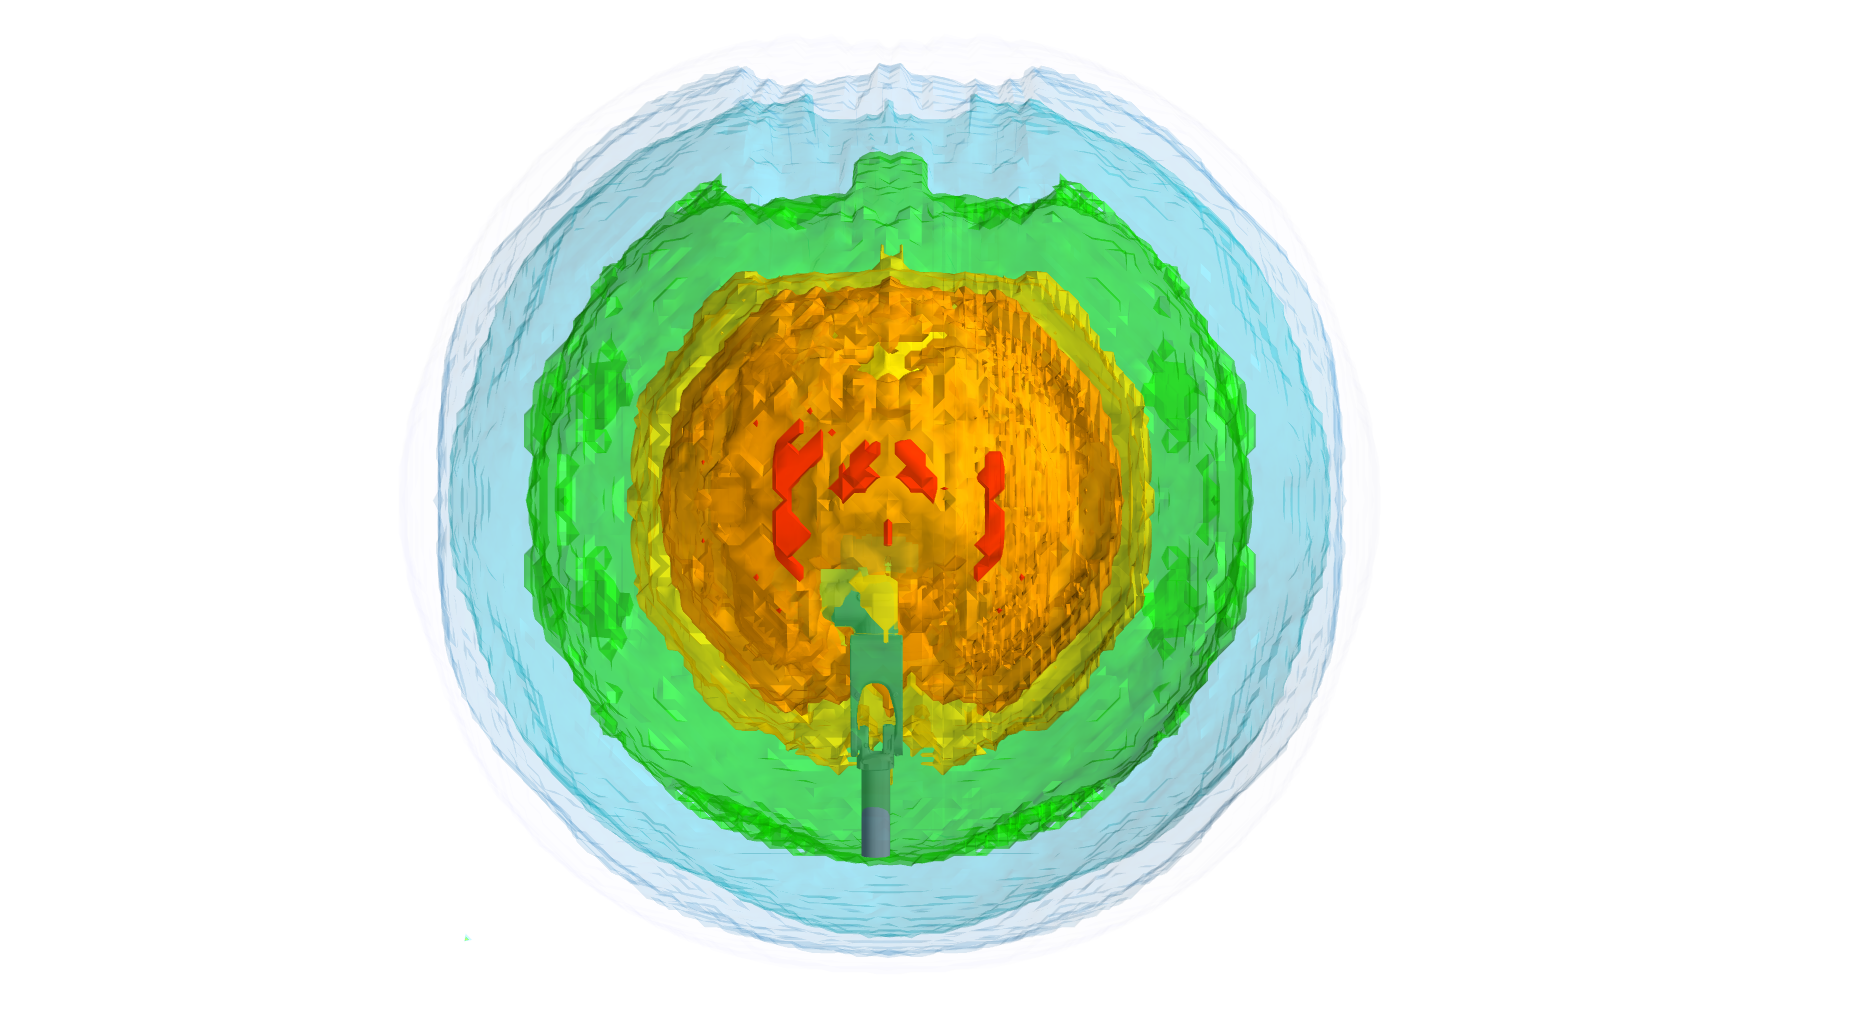
\includegraphics[width=\columnwidth]{detail/figs/bighatch/mh12_top.png}
	\caption{Espaço de trabalho do manipulador MH12 - vista superior}
	\label{fig::mh12cin2}
\end{figure}

\begin{figure}[h!]	
	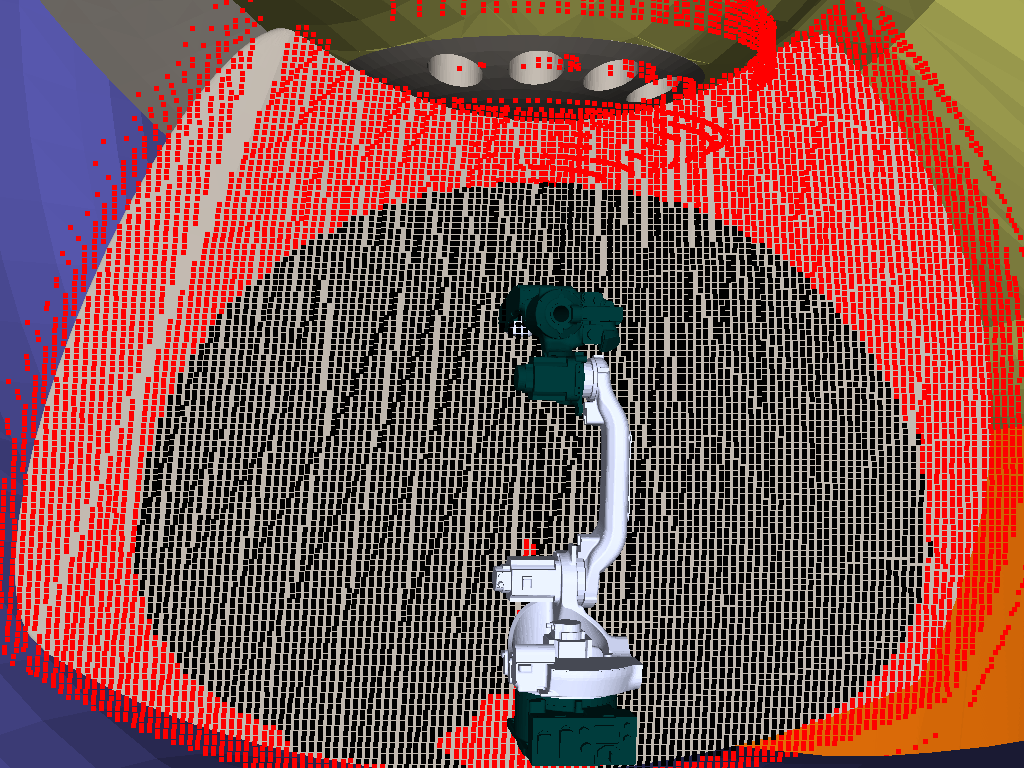
\includegraphics[width=\columnwidth]{detail/figs/bighatch/mh12_bestpos.png}
	\caption{Melhor posição para o revestimento - robô MH12 da Motoman.}
	\label{fig::mh12bestpos}
\end{figure}


\paragraph{LBR iiwa 14 R820 (Kuka)}
O manipulador LBR iiwa 14 R820 possui 7 graus de liberdade e, devido a sua
grande flexibilidade e facilidade de montagem, foram estudadas duas
configurações para a base.

O script que calcula a melhor posição da base na posição vertical em relaçao à
pá retornou a posição 1.06, sendo que 2648 pontos foram revestidos,
representando 17.20\% de toda a pá. Estima-se que serão necessários, pelo menos,
13 posições para o recobrimento de toda a pá, figura~\ref{fig::lbrbestposv}.

\begin{figure}[h!]	
	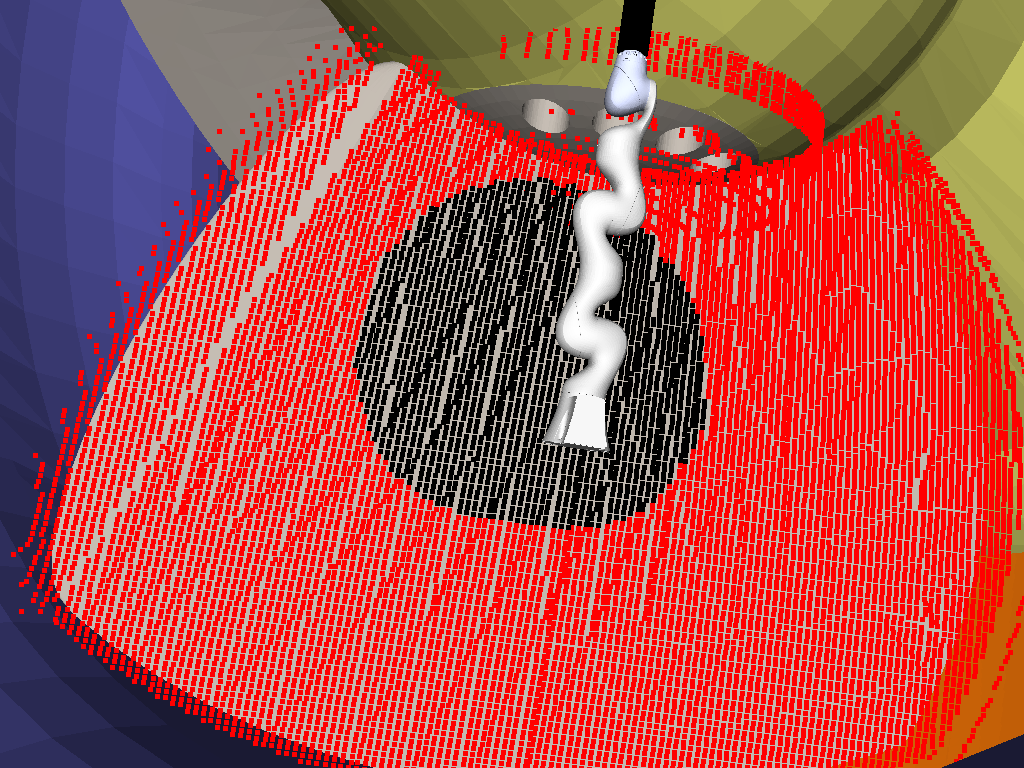
\includegraphics[width=\columnwidth]{detail/figs/bighatch/lbr_bestposv.png}
	\caption{Melhor posição para o revestimento - robô LBR da Kuka com base na
	posição vertical.}
	\label{fig::lbrbestposv}
\end{figure}

O script que calcula a melhor posição da base na posição vertical em relaçao à
pá retornou a posição 1400 mm, sendo que 2730 pontos foram revestidos,
representando 17.37\% de toda a pá. Estima-se que serão necessários, pelo menos,
13 posições para o recobrimento de toda a pá, figura~\ref{fig::lbrbestposh}.

\begin{figure}[h!]	
	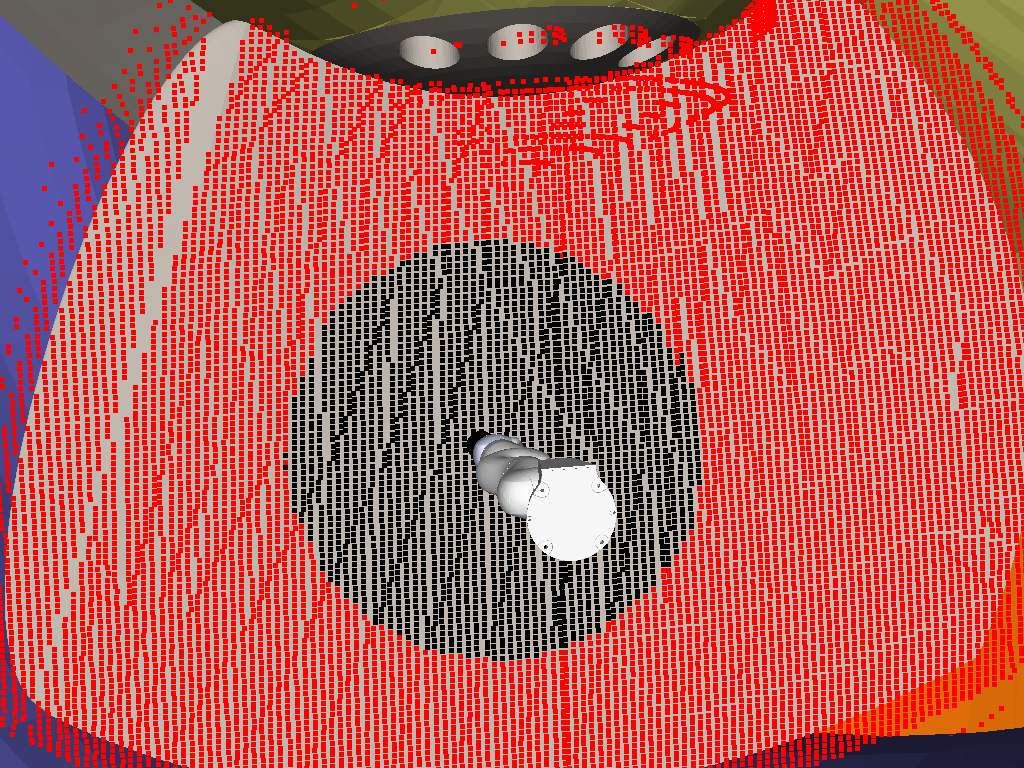
\includegraphics[width=\columnwidth]{detail/figs/bighatch/lbr_bestposh.png}
	\caption{Melhor posição para o revestimento - robô LBR da Kuka com base na
	posição horizontal.}
	\label{fig::lbrbestposh}
\end{figure}

\paragraph{SIA20D (Motoman)}
O manipulador SIA20D também possui 7 graus de liberdade e, devido a sua
grande flexibilidade e facilidade de montagem, foram estudadas duas
configurações para a base.

O script que calcula a melhor posição da base na posição vertical em relaçao à
pá retornou a posição 1100 mm, sendo que 3638 pontos foram revestidos,
representando 23.14\% de toda a pá. Estima-se que serão necessários, pelo menos,
9 posições para o recobrimento de toda a pá, figura~\ref{fig::sia20dbestposv}.

\begin{figure}[h!]	
	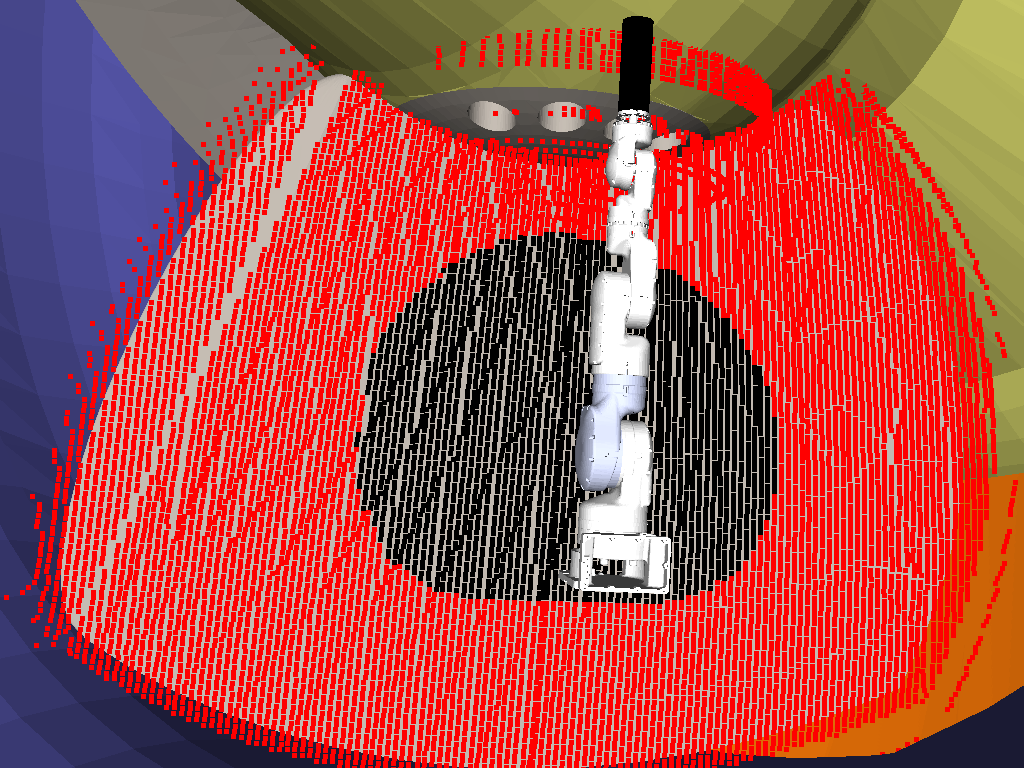
\includegraphics[width=\columnwidth]{detail/figs/bighatch/sia20d_bestposv.png}
	\caption{Melhor posição para o revestimento - robô SIA20D da Motoman com base
	na posição vertical.}
	\label{fig::sia20dbestposv}
\end{figure}

O script que calcula a melhor posição da base na posição horizontal em relaçao à
pá retornou a posição 1510 mm, sendo que 3892 pontos foram revestidos,
representando 24.76\% de toda a pá. Estima-se que serão necessários, pelo menos,
9 posições para o recobrimento de toda a pá, figura~\ref{fig::sia20dbestposh}.

\begin{figure}[h!]	
	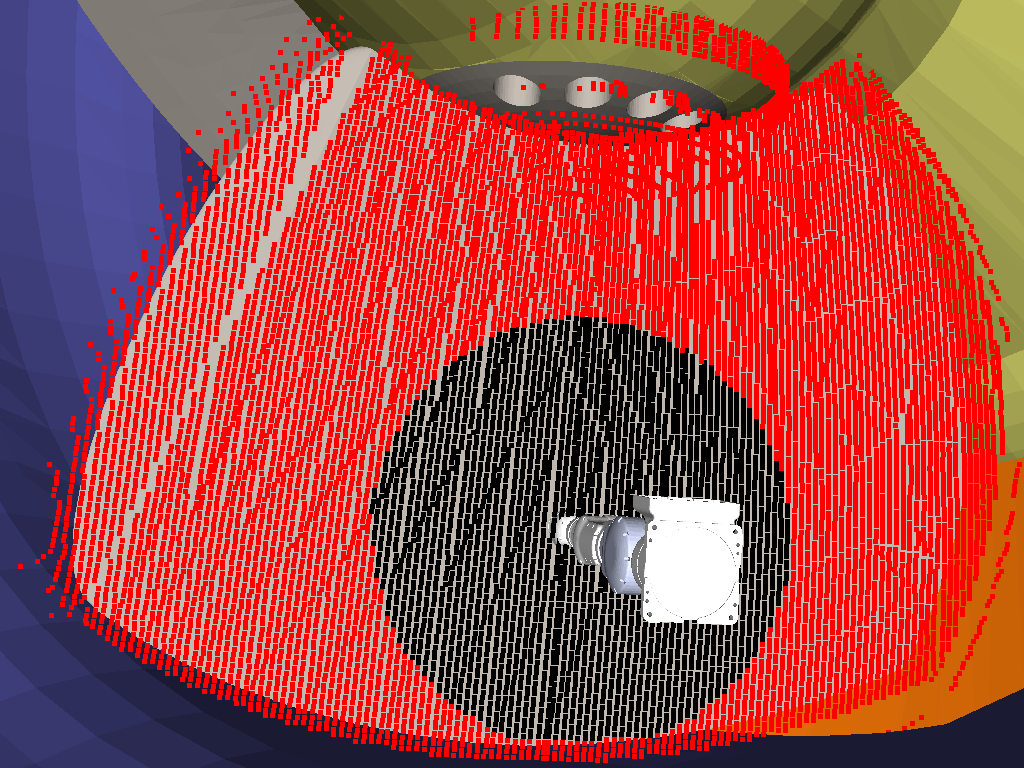
\includegraphics[width=\columnwidth]{detail/figs/bighatch/sia20d_bestposh.png}
	\caption{Melhor posição para o revestimento - robô SIA20D da Motoman com base
	na posição horizontal.}
	\label{fig::sia20dbestposh}
\end{figure}

\paragraph{Tolerância no ângulo de revestimento}
As análises de revestimento dos manipuladores exigiram que a pistola
estivesse com as mesmas direções e sentidos opostos às normais dos
pontos a serem revestidos, isto é, a orientação da pistola é sempre
perpendicular ao plano da pá. Entretanto, pode-se assumir uma tolerância de
$90^o \pm 60^o$ entre a pistola e o plano perpendicular, que foi considerada
na análise puramente geométrica. Como o manipulador MH12 (Motoman) possui
recobrimento de quase todo o alcance vertical da pá (revestimento de cima a
baixo), mostra-se interressante a análise de tolerância neste manipulador, de
forma que haja simplificação das possíveis soluções de bases.

Primeiramente, são armazenados os pontos que o robô não foi capaz de
revestir (pontos em vermelho, nas figuras de espaço de trabalho dos
manipuladores) e suas respectivas normais aos planos tangentes à superfície da
pá. Os pontos são deslocados 230 mm na mesma direção e sentido oposto às suas
respectivas normais, de forma que pertençam à superfície da pá,
ponto $D$ é deslocado até ponto $C$ na figura~\ref{fig::tolerancia1}. Para cada
ponto não revestido, são gerados dois vetores unitários $\overrightarrow{v}$ e
$\overrightarrow{w}$ ortogonais entre si e ao vetor normal $\overrightarrow{N}$,
no plano tangente à superfície da pá, conforme
ilustrado na figura~\ref{fig::tolerancia2}. O vetor $\overrightarrow{N}$ é
girado pelo ângulo de tolerância de revestimento $\theta$ (entre $0^o$ e $60^o$)
em relação ao vetor $\overrightarrow{w}$, gerando o vetor
$\overrightarrow{P_1}$, figura~\ref{fig::tolerancia3}.

\begin{figure}[h!]	
	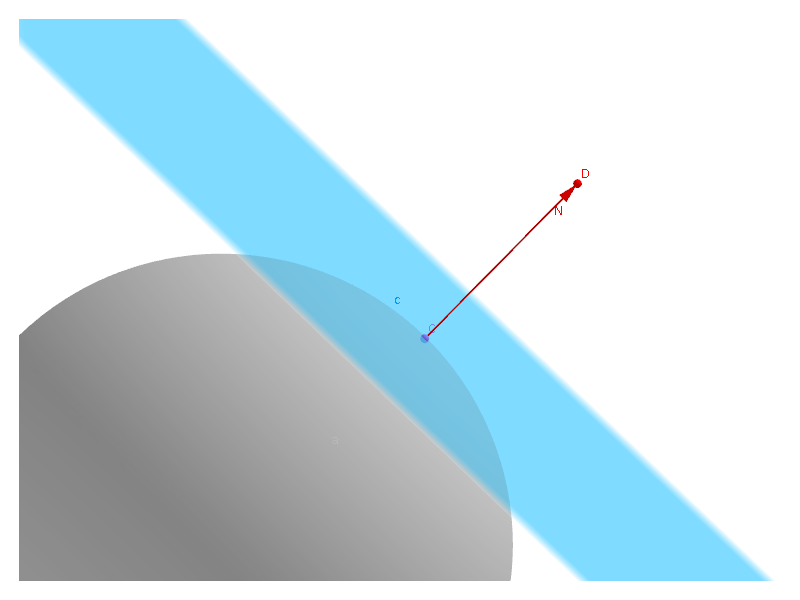
\includegraphics[width=\columnwidth]{detail/figs/bighatch/tolerancia1.png}
	\caption{Ponto D não revestido, deslocado 230 mm da superfície da pá.}
	\label{fig::tolerancia1}
\end{figure}

\begin{figure}[h!]	
	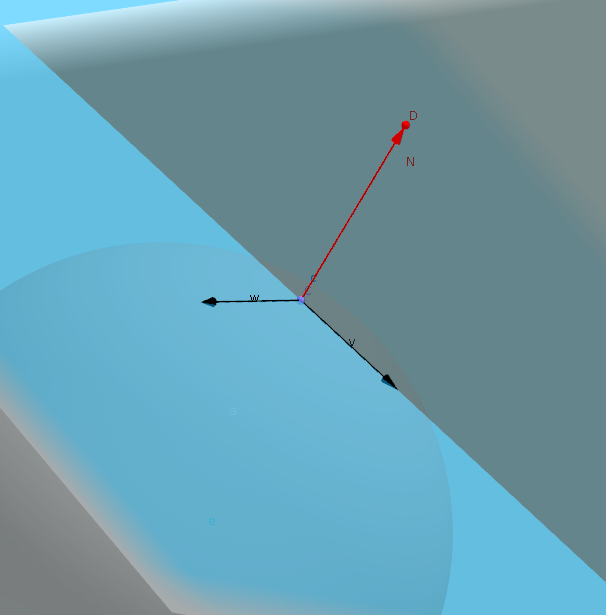
\includegraphics[width=\columnwidth]{detail/figs/bighatch/tolerancia2.png}
	\caption{Vetores v e w ortogonais ao vetor normal N.}
	\label{fig::tolerancia2}
\end{figure}

Finalmente, o vetor $\overrightarrow{P_1}$ pode ser girado em relação a
$\overrightarrow{N}$ e todos os vetores que pertencem à tolerância de
revestimento $\theta$ saem do ponto $C$ até um ponto do círculo $h$, como o
vetor exemplo $\overrightarrow{P_2}$, na figura~\ref{fig::tolerancia4}. Observe
que este círculo deve ser discretizado, e cada ponto pertencente ao círculo e sua
respectiva normal (vetor de origem $C$ ao ponto do círculo) devem ser
reavaliados, isto é, verifica-se se o robô alcança o ponto pertencente a $h$ com
pistola de revestivemto apontada a sua respectiva normal.
Se algum ponto do círculo puder ser revestido, o ponto $D$ pode ser considerado
como revestido. No exemplo da figura~\ref{fig::tolerancia4}, o círculo $h$ foi
discretizado em dois pontos $G$ e $H$, e suas normais são $\overrightarrow{P_1}$
e $\overrightarrow{P_2}$, respectivamente. 

\begin{figure}[h!]	
	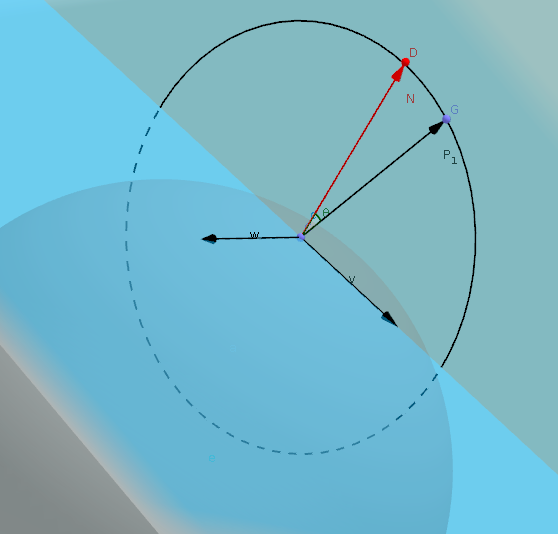
\includegraphics[width=\columnwidth]{detail/figs/bighatch/tolerancia3.png}
	\caption{Vetor N girado pelo ângulo de tolerância de revestimento.}
	\label{fig::tolerancia3}
\end{figure}

\begin{figure}[h!]	
	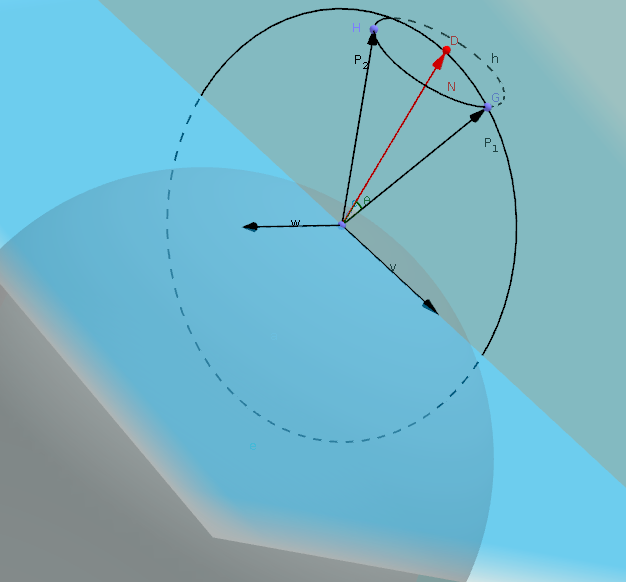
\includegraphics[width=\columnwidth]{detail/figs/bighatch/tolerancia4.png}
	\caption{Circulo $h$ representa todos os pontos equivalentes ao ponto $D$ com
	ângulo de tolerância de revestimento $\theta$.}
	\label{fig::tolerancia4}
\end{figure}

Foram realizadas análises de tolerância para dois robôs: MH12, que apresentou o
maior número de pontos revestido na pá, e LBR R820, que é a única solução viável
de manipulador industrial para o acesso superior. Os ângulos de tolerância foram
variados em $10^o$ e $30^o$. 

\subsection{Dinâmica do manipulador}\label{sec::dinamica}
% Author: Renan

A dinâmica de um manipulador robótico é a análise de velocidades, acelerações e
torques das juntas. Para esta análise, assume-se que o efetuador, pistola de
revestimento, possui velocidade 40m/min constante em todos os pontos amostrados
da pá. Como velocidades e acelerações exigem a computação de derivadas, é
realizada uma melhor discretização da pá da turbina, na qual o passo de
amostragem é menor e um filtro garante espaçamento uniforme dos pontos de 10 mm.
Para um lado da pá, são amostrados, portanto, 130 mil pontos.

Para cada ponto amostrado da pá, faz-se a análise cinemática e são armazenados
os pontos que são possíveis de serem revestidos, como na
seção~\ref{sec::cinematica}, isto é, são armazenados os pontos que possuem
solução de cinemática inversa. Posteriormente, para cada ponto revestido, é
criado um conjunto contendo seus 8 pontos vizinhos através de um algoritmo k-d
tree, como na figura~\ref{fig::pontosdin}, onde $p_r$ é o ponto de referência a
ser analisado dinamicamente e os pontos ${p_1,p_2,q_1,q_2,r_1,r_2,s_1,s_2}$ são auxiliares
para o estudo. 

\begin{figure}[h!]	
	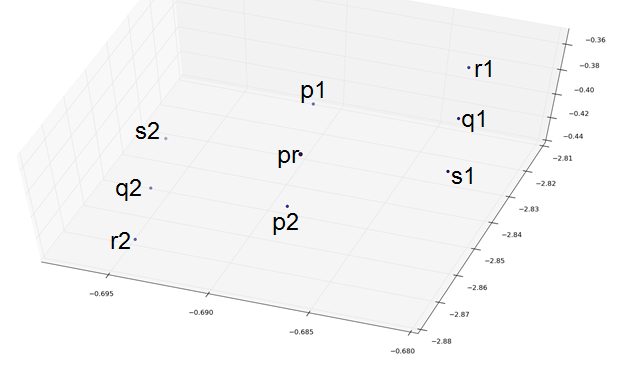
\includegraphics[width=\columnwidth]{detail/figs/dinamica/pontosdinamica.png}
	\caption{Pontos exemplo amostrados da pá.}
	\label{fig::pontosdin}
\end{figure}

%As soluções de cinemática inversa (ângulos das juntas do robô)
%$\Theta_r
%=
%{\theta_{p_r},\theta_{p_1},\theta_{p_2},\theta_{q_1},\theta_{q_2},\theta_{r_1},\theta_{r_2},\theta_{s_1},\theta_{s_2}}$
As velocidades angulares das juntas são calculadas a partir da cinemática
diferencial. Para isso, usa-se o cálculo da matriz jacobiana ($J$), que é a
diferenciação (derivadas parciais) da matriz de cinemática direta em função das
variáveis de junta \citep{sciavicco2000differential}. A velocidade linear do
efetuador ($\dot{X}$) e o jacobiano são conhecidos em cada ponto de referência, logo
podem-se calcular as velocidades das juntas do manipulador entre o ponto de
referência e cada ponto auxiliar: $\dot{X} = J\dot{q}\Rightarrow
J^+\dot{X}=\dot{q}$, onde $J^+$ é a pseudo inversa Moore-Penrose de $J$.

As velocidades angulares são $\Omega_r
=
\{\omega_{p_r,p_1},\omega_{p_r,p_2},\omega_{p_r,q_1},\omega_{p_r,q_2},\omega_{p_r,r_1},\omega_{p_r,r_2},\omega_{p_r,s_1},\omega_{p_r,s_2}\}$,
onde $\omega$, $\omega\in\Omega_r$, é um vetor $n \times 1$, e $n$ é o número de
juntas do robô. As velocidades dos ângulos das juntas é uma informação importate para a
verificação da viabilidade das trajetórias do robô. Para o caso do robô
MH12, onde $\omega_{\textbf{max}}=\{220, 200, 220, 410, 410, 610\}^o/s$, por
exemplo, caso não haja $\omega\in\Omega_r$, tal que
$\omega\leq\omega_{\textbf{max}}$, não é possível realizar o revestimento do
ponto de referência $p_r$. Se $\exists \omega\in\Omega_r$ tal que
$\omega\leq\omega_{\textbf{max}}$, o ponto de referência é viável pela
cinemática inversa e pela cinemática diferencial, mas pode ser inviável ainda
pela análise dinâmica, que considera as acelerações, massas e forças do
conjunto.

As equações dinâmicas de um manipulador são também abordados em
\cite{sciavicco2000differential} e possuem duas abordagens bem conhecidas na
literatura: equações de Newton-Euler e equações de Lagrange. O ambiente OpenRave
utiliza o método de Newton-Euler para computar os torques das juntas (dinâmica
inversa): $\tau = M(q)\alpha + C(q,\omega)\omega + G(q) $, onde $\tau$ é o
vetor de torques das juntas, $M$ matriz de massas e momentos de inércia,
$\alpha$ é acelerações das juntas, $C$ matriz de Coriolis, $\omega$ é as
velocidades das juntas e $G$ o vetor de gravidade.

Para a formação da matriz $M$, é necessária a estimação de parâmetros do
manipulador. A estimação dos parâmetros pode ser realizada de maneira iterativa,
isto é, aplicam-se torques nas juntas e, pela resposta
do manipulador, estima-se a matriz \citep{slotine1988adaptive}; ou pelo CAD do
manipulador, por exemplo, pela utilização da ferramenta SolidWorks. Foi utilizado o método de estimação pelo CAD do
manipulador, visto que os manipuladores ainda estavam em estudo e não foram
adquiridos, além disso houve facilidade de aproximar os parâmetros já que o CAD
fornecido pelo fabricante é bem detalhado. 

A aceleração angular, $\alpha$, é necessária para a computação dos torques,
$\tau$. O método analítico para cálculo da aceleração angular das juntas é
através da derivada da equação da cinemática diferencial:
$\ddot{X}=\dot{q}^TH\dot{q}+J\ddot{q} \Rightarrow
\ddot{q}=J^+(\ddot{X}-\dot{q}^TH\dot{q})$ ou
$\alpha=J^+(a-\omega^TH\omega)$, onde $H$ é a matriz Hessiana, isto é, derivada
parcial da matriz jacobiana $J$ \citep{hourtash2005kinematic}. 

Com a informação dos ângulos, velocidades e acelerações das juntas, momentos
de inércia e massa dos elos, o OpenRave calcula a dinâmica inversa através do
método Newton-Euler, obtendo-se os torques. Para cada ponto de referência, há quatro direções
(trajetórias) possíveis amostradas que o efetuador pode percorrer:
$\{(p_1,p_r,p_2),(q_1,p_r,q_2),(r_1,p_r,r_2),(s_1,p_r,s_2)\}$, logo quatro
ângulos, velocidades e acelerações de juntas, portanto são obtidos quatro
possíveis vetores de torques:
$T=\{\tau_{rp},\tau_{rq},\tau_{rr},\tau_{rs}\}$. E, especificamente para o
caso do manipulador MH12, os valores dos torques devem ser inferiores aos
estabelecidos pelo datasheet:
$\tau_{\textbf{max}}=\{-,-,-,22,22,9.8\}\textbf{Nm}$, logo se $\exists \tau\in
T$, tal que $\tau\leq\tau_{\textbf{max}}$, então há uma trajetória viável.

As figuras~\ref{fig::wgeo}, ~\ref{fig::wcin} e ~\ref{fig::wdin} representam a
evolução das análises do manipulador, de um nível mais simples a um nível mais
complexo de detalhamento, o qual avalia velocidades, acelerações e torques das
juntas do manipulador. Ainda deverá ser executada a análise de manipulabilidade
que avalia o sistema de controle do manipulador. Esta análise é importante para
o planejamento de trajetórias do manipulador e para o cálculo das posições
viáveis da base para uma operação completa.



\begin{figure}[h!]	
	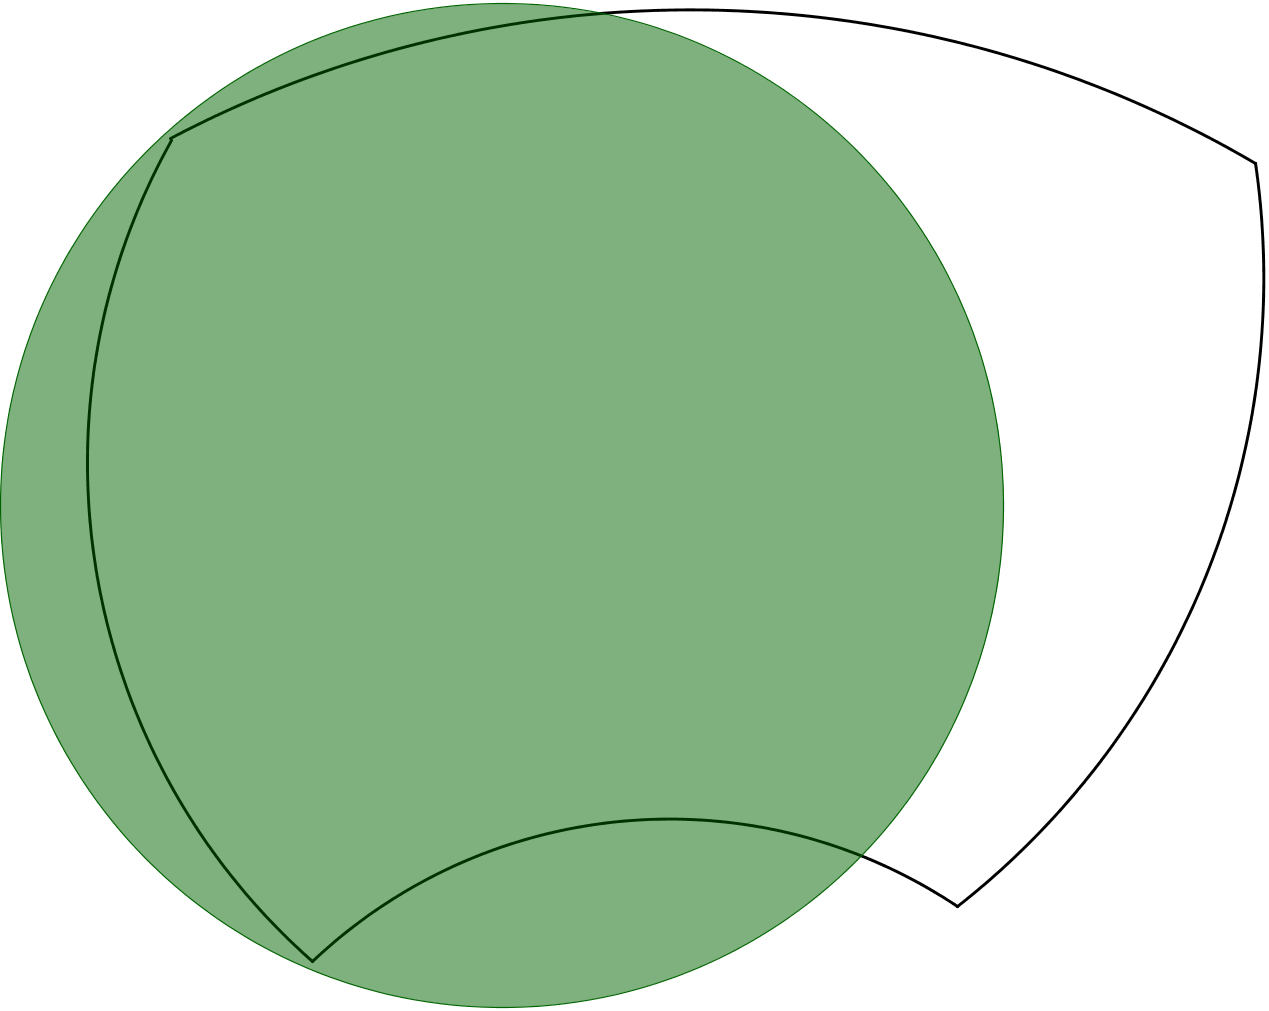
\includegraphics[width=\columnwidth]{detail/figs/dinamica/workspaceGeometrico.png}
	\caption{Área em verde representa a cobertura do revestimento executada pelo
	manipulador, utilizando a abordagem puramente geométrica.}
	\label{fig::wgeo}
\end{figure}

\begin{figure}[h!]	
	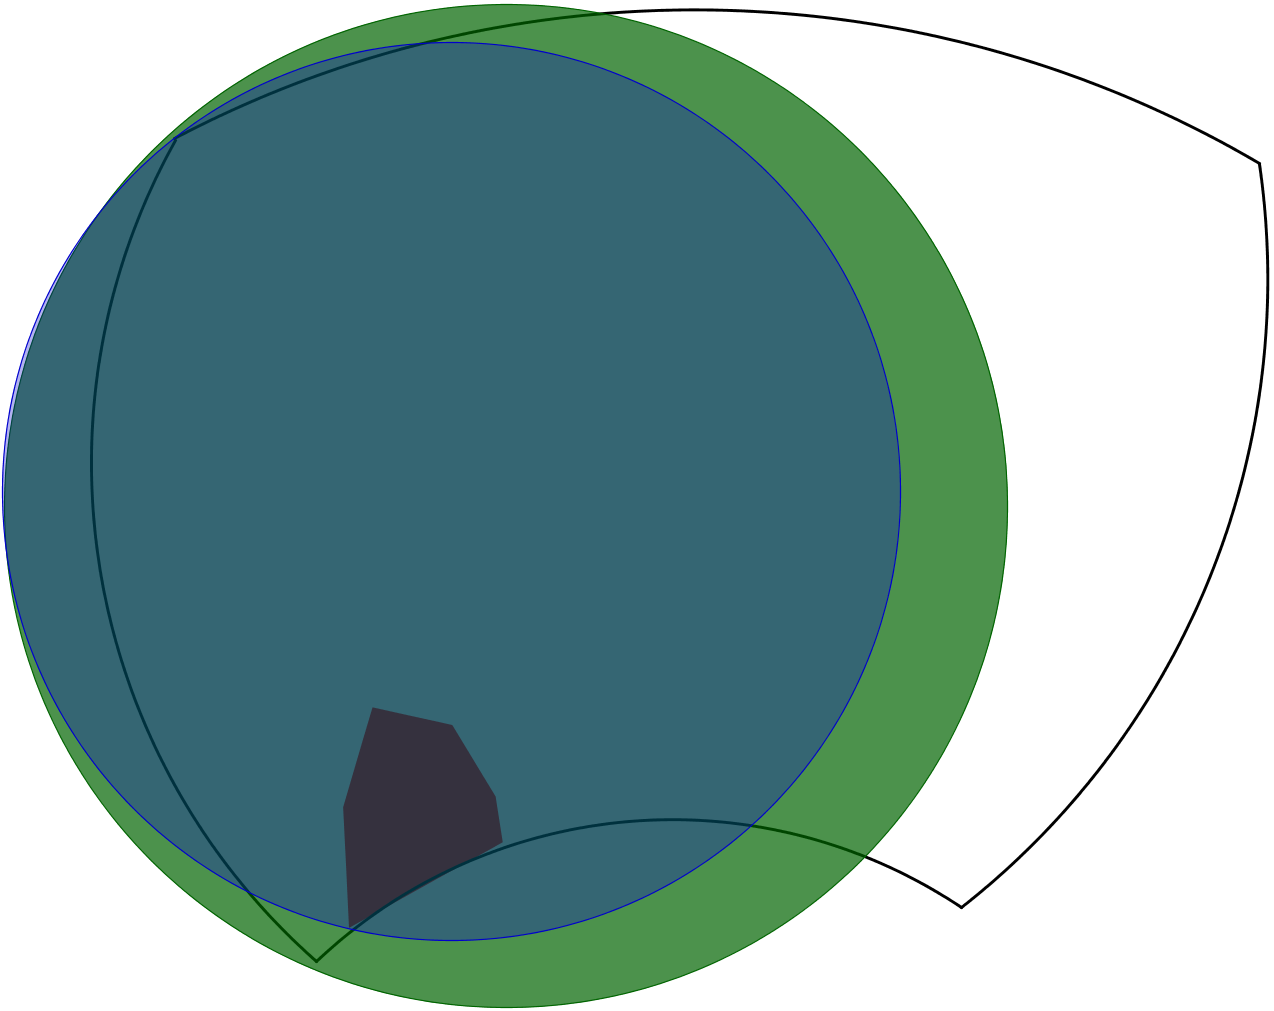
\includegraphics[width=\columnwidth]{detail/figs/dinamica/workspaceCinematica.png}
	\caption{Área em verde representa a cobertura do revestimento executada pelo
	manipulador, utilizando a abordagem puramente cinemática.}
	\label{fig::wcin}
\end{figure}

\begin{figure}[h!]	
	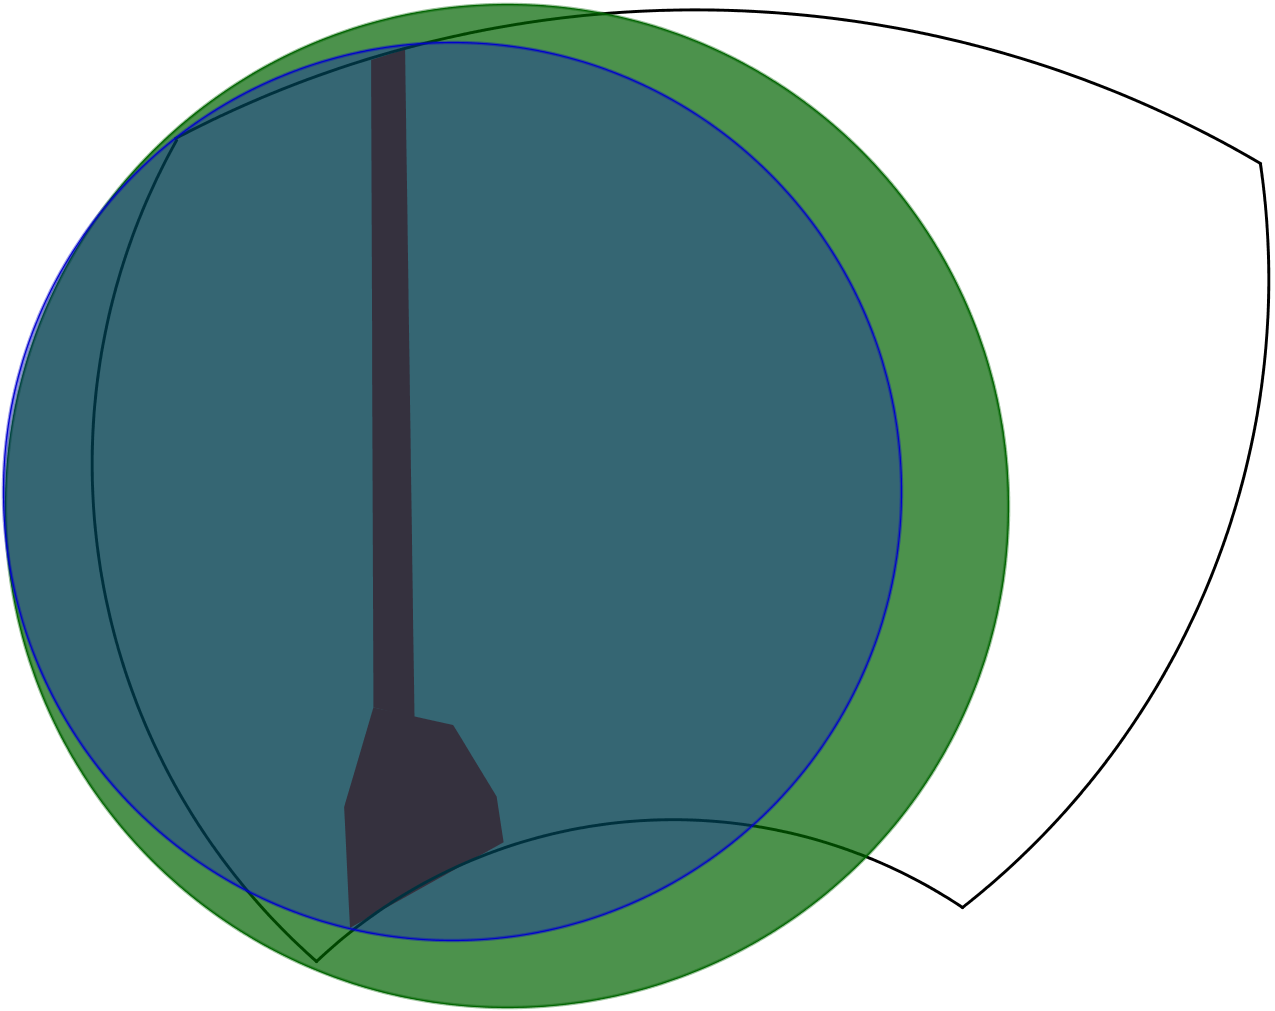
\includegraphics[width=\columnwidth]{detail/figs/dinamica/workspaceTorques.png}
	\caption{Área em verde representa a cobertura do revestimento executada pelo
	manipulador, utilizando a abordagem dinâmica.}
	\label{fig::wdin}
\end{figure}
\subsection{Detalhamento da Base Mecânica}\label{sec::base_mec}
A base mecânica é composta pelos elementos de suporte, transporte e ancoragem do
robô no interior da turbina. Os elementos de suporte formam a estrutura
principal da base, que estruturam o ambiente para a montagem, movimentação e
funcionamento seguros do robô. Os elementos de transporte oferecem ao
manipulador graus de liberdade que permitem que este se posicione com facilidade
nos pontos ótimos para o processo. Estes elementos podem ser trilhos, atuadores
lineares, mancais de rolamento, atuadores rotativos, etc. Já os elementos de
ancoragem são necessários para fixar o robô e a estrutura no ambiente. As
opções de ancoragem estudadas foram as bases magnéticas e solda. A
primeira opção, bases magnéticas, é de preferência pois não danifica o ambiente
e não necessita de outros equipamentos para montagem. No caso da solda,
seriam necesários um soldador capacitado e os equipamentos de soldagem no interior do
ambiente confinado, quando a opção da base magnética não requer equipamentos
extras.

As etapas de detalhamento da base mecânica seguem a seguinte ordem: $1)$
investigação dos graus de liberdade necessários; $2)$ configuração conceitual 
da base em função dos graus de liberdade; $3)$ escolha do melhor conceito; $4)$ 
escolha e dimensionamento dos elementos mecânicos que compõem a base; $5)$ testes.
Avaliamos até esta etapa do projeto os itens: $1$,$2$ e $3$.

Os graus de liberdade são fornecidos através de combinações de juntas
prismáticas e rotacionais, que no nosso caso irão permitir o movimento do robô
desde a escotilha inferior até o ponto de interesse, tanto para o início do
processo de revestimento em uma região da peça, como para a movimentação de
precisão para a região seguinte.
Investigou-se primeiramente alguns conceitos baseados nos graus de liberadade 
necessários para fornecer à base do robô todos os posicionamentos necessários, 
de acordo com os estudos cinemáticos e dinâmicos descritos  nas
seções~\ref{sec::cinematica} e \ref{sec::dinamica}. Estes conceitos serão
apresentados em detalhe na seção~\ref{sec::conceitos_base}.
%TODO criar label para sec estudo dinamico

A análise dos conceitos estudados permite então compara-los e definir o que
melhor se adapta ao objetivo da solução. Nesta etapa incia-se o detalhamento da base
mecânica seguindo as diretrizes e requisitos mecânicos do projeto. A
estrutura deve ter capacidade de suportar os esforços dinâmicos do robô,
de forma que não haja grandes deformações elásticas e oscilações que possam
comprometer a precisão de posicionamento do efetuador do braço robótico.
Deve-se atentar também ao caráter dinâmico dos esforços, que causam vibrações
que podem resultar em esforços e deslocamentos elevados.
Assim, a fixação da estrutura da base no ambiente deve ser o mais rígida
possível, superdimensionando os elementos de ancoragem e minimizando as folgas
nos acoplamentos. A próxima etapa do projeto é justamente dimensionar a
estrutura mecânica a partir do conceito escolhido.

\subsubsection{Conceitos de base mecânica}\label{sec::conceitos_base}
A seguir apresenta-se os conceitos analisados, em relação aos graus de
liberdade da base mecânica:

$\bullet$~\textbf{Base Prismática-Rotacional-Rotacional (P-R-R):}
  
  Neste conceito estudou-se a possibilidade de utilizar uma base com $3$ graus
  de liberdade: um prismático e dois rotacionais. O prismático seria composto
  por um trilho alinhado e paralelo ao eixo da turbina que transportaria o robô
  até a região próxima a pá. Uma junta rotacional e com eixo vertical orientaria
  a base nesta direção e uma junta perpedincular à primeira faria o
  posicionamento da base do robô para então iniciar o processo de revestimento.
  A figura~\ref{fig::base_prr} ilustra este conceito.
    
  \begin{figure}[h!]
   \centering
   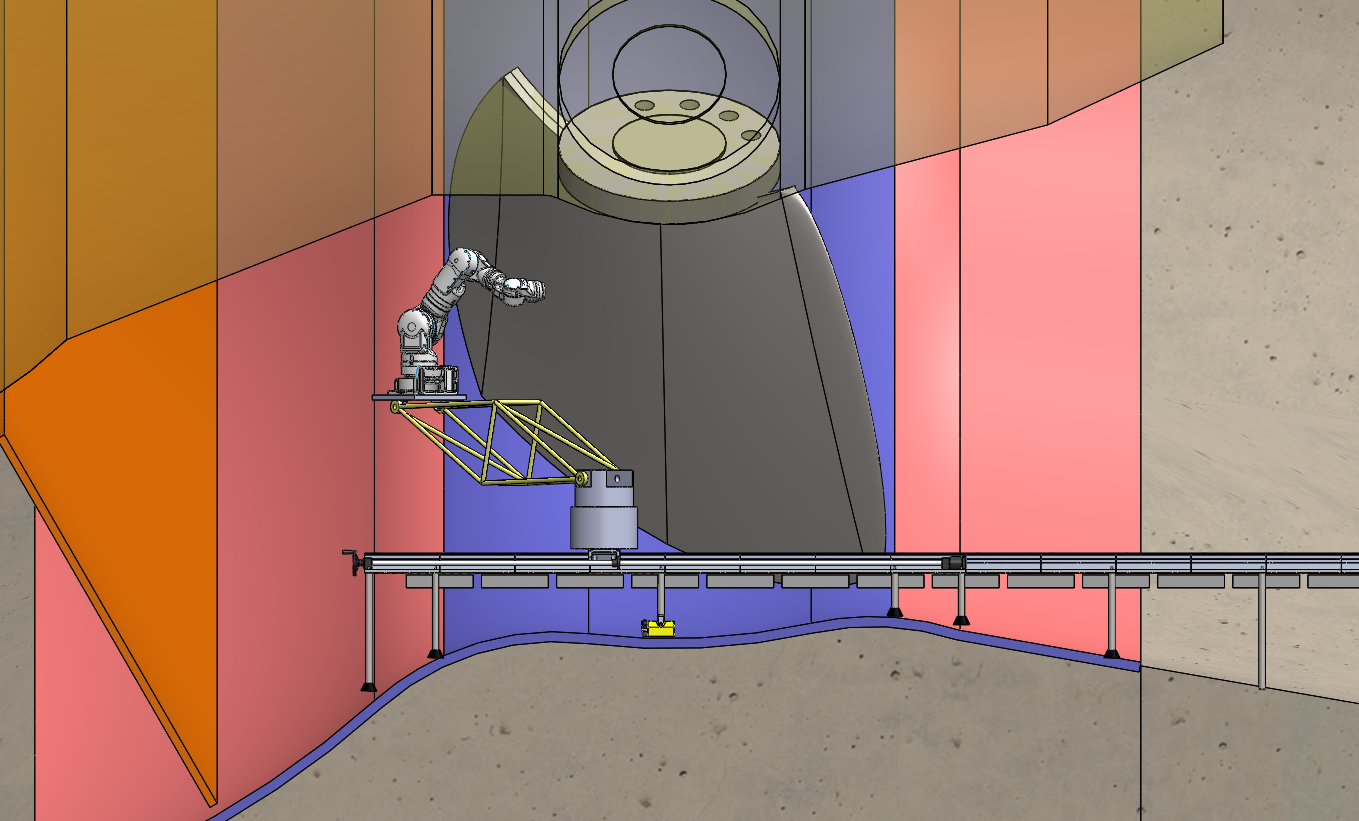
\includegraphics[width=\columnwidth]{detail/figs/bases/base_prr}
   \caption{Base Primático-Rotacional-Rotacional}
   \label{fig::base_prr}
\end{figure}

  A vantagem deste conceito é conferir um alcance grande ao manipulador através
  da base, permitindo que este possa ser de menor alcance próprio, mas ao mesmo
  tempo mais leve.
  Porém, devido à configuração de juntas e pelos resultados encontrados no
  estudo cinemático, a manobrabilidade desta base seria reduzida naquele espaço,
  havendo posicionamentos difíceis de serem alcançados, ou até impossíveis
  dependendo do manipulador escolhido.
  
$\bullet$~\textbf{Base Prismática (P):}

  Este conceito consiste de um trilho (junta prismática) para o transporte do
  manipulador desde a escotilha até o ponto de interesse para revestimento na
  face anterior ou posterior da pá. Quando posicionado, remove-se a seção
  do trilho na direção que obstrui a rotação do rotor. Neste conceito,
  adiciona-se um grau de liberdade ao sistema utilizando a própria rotação do
  rotor, posicionando a pá em relação ao robô. A base mecânica então forneceria
  apenas movimento no trilho na direção do eixo da turbina, deixando fixas as
  outras direções. O procedimento para o revestimento seria o posicionamento do
  rotor, deixando a região a ser processada ao alcance do manipulador; o
  posicionamento do robô no trilho, em relação a pá; a ancoragem do robô
  no ambiente; e o revestimento da região possível para aquela posição.
  Repete-se então este procedimento até ter toda a face processada e
  posiciona-se a próxima pá para revestimento, sem necessidade de mover ou
  desmontar a base do robô até todas as faces daquele lado estarem completas.  A
  figura~\ref{fig::base_p} ilustra este conceito.
  
  \begin{figure}[h!]
   \centering
   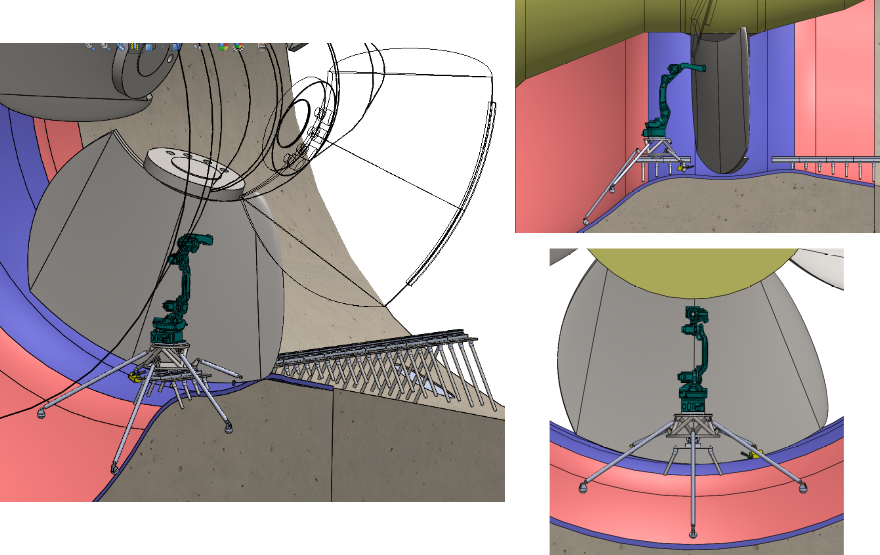
\includegraphics[width=\columnwidth]{detail/figs/bases/base_p}
   \caption{Base Prismática}
   \label{fig::base_p}
\end{figure}
  
  Este conceito foi estudado para o manipulador MH$12$, que de acordo com a
  análise cinemática consegue processar toda a extensão vertical. Para outros
  manipuladores, seria necessário incluir uma junta prismática, adicionando um
  grau de liberdade, na direção vertical.
  
  A análise cinemática também demonstrou que seriam necessárias muitas posições
  do rotor para completar uma face da pá. Há inclusive dificuldades operacionais e
  de segurança no procedimento de rotação do rotor que devem ser considerados. O
  rotor só pode ser girado manualmente, não fornecendo precisão no
  posicionamento da pá em relação a base. Por ser uma tarefa manual, deve-se ter
  procedimentos adequados de segurança para preservar tanto o operador quanto os
  equipamentos próximos. Estas preocupações tornam a solução pouco prática sob o
  ponto de vista operacional.

$\bullet$~\textbf{Base Prismática-Rotacional-Prismática (P-R-P):}

  Este conceito consiste de uma base composta por um trilho primário (junta
  prismática $1$), uma plataforma de base pivotada por mancal e rolamentos entre
  o trilho primário e secundário (junta rotacional) e um trilho secundário
  (junta prismática $2$). Montado o trilho primário alinhado ao eixo da turbina
  a base rotacional sobre o trilho primário, fixa-se o robo sobre a base
  rotacional. Esta base permitrá a montagem do trilho secundário apenas quando o
  robô atingir a região de interesse para revestimento. Quando posicionado o
  manipulador, monta-se então o trilho secundário alinhado ao plano paralelo a
  face da pá e ancora-se a base no ambiente. Desta forma, o robô pode-se
  movimentar ao longo de toda a extensão da pá por meio do trilho secundário e
  também se aproximar e se afastar da superfície da pá, por meio do trilho
  primário. A figura~\ref{fig::base_prp} ilustra este conceito.

\begin{figure}[h!]
   \centering
   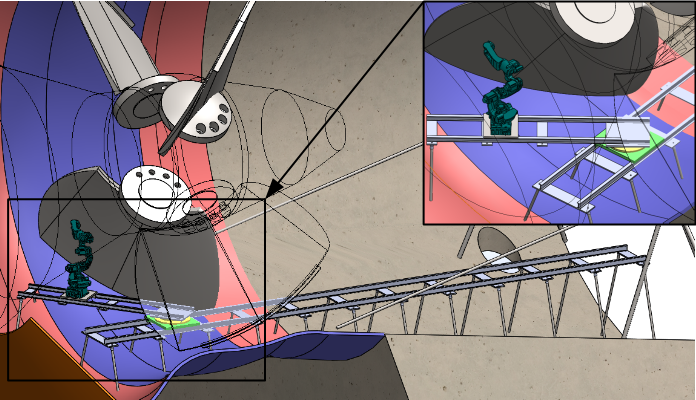
\includegraphics[width=\columnwidth]{detail/figs/bases/base_prp}
   \caption{Base Primática-Rotacional-Prismática}
   \label{fig::base_prp}
\end{figure}

  Desta forma, o rotor deve estar girado em, no mínimo $30^o$ para não haver
  contato com o trilho primário. A análise cinemática será realizada para
  encontrar a melhor configuração de juntas da base que permite ao robô se
  movimentar nos graus de liberdade da base, sem alterar o posicionamento do
  rotor e, assim, cobrir uma face inteira da pá. Para a repetição do processo
  nas outras pás do lado da sucção da turbina, é necessária a desmontagem do
  trilho secundário, o recuo do robô e desmontagem de parte do trilho primário,
  permitindo o giro do rotor para a pá seguinte.
  Para as faces do lado de adução, não é necessária a desmontagem parcial do
  trilho primário.
  
\subsubsection{Sistemas de elevação, fixação e ancoragem}
A entrada dos componentes da base mecânica é uma tarefa trabalhosa, devido ao
acesso limitado ao interior da turbina. O diâmetro de $800~mm$ da escotilha
inferior limita o tamanho e geometria dos equipamentos, fazendo com que estes
tenham dimensões reduzidas.
Estes componentes devem ser içados até a escotilha em uma altura de $5~m$ entre
o piso no exterior do ambiente confinado e seu interior. Assim, a modularidade dos elementos que compõe a base
é uma diretriz essencial a esse projeto. A estratégia então é ter-se pequenos módulos de componentes
que poderão ser içados separadamente e acoplados entre si, até se obter a
estrutura completa. 
A facilidade de transporte, montagem e desmontagem da base mecânica causará um
grande impacto na praticidade e agilidade de implementação da solução.

A entrada de pessoal através da escotilha é feita por uma escada vertical com
guarda-corpo. Equipamentos de segurança como
cinto e talabarte devem ser usados para qualquer um que deseja entrar no
ambiente confinado da turbina através da escada e isso impossibilita o
transporte manual dos equipamentos. Por este motivo, deve ser instalada uma
estrutura com talha que permita a elevação até o interior da turbina e
movimentação para a áera de montagem adequada. As figuras~\ref{fig::talha} e
\ref{fig::talha_trilho} ilustram a estrutura de elevação com talha e carro
trole. 
  
\begin{figure}[h!]
   \centering
   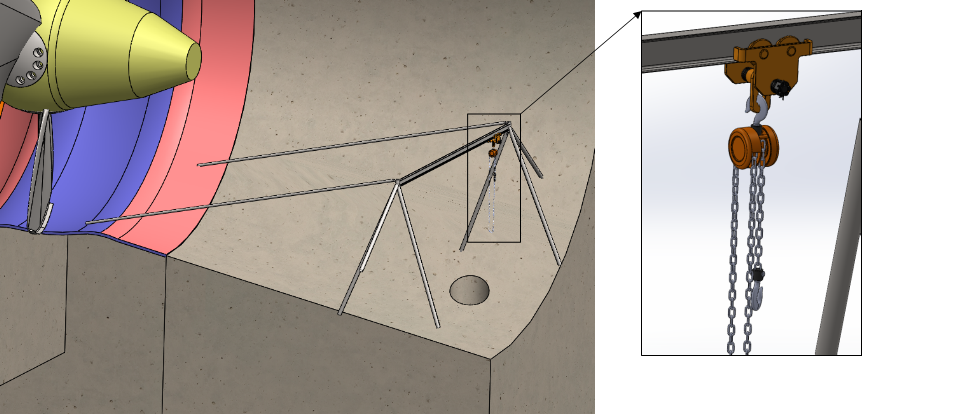
\includegraphics[width=\columnwidth]{detail/figs/bases/talha}
   \caption{Sistema de elevação dos equipamentos}
   \label{fig::talha}
\end{figure}

\begin{figure}[h!]
   \centering
   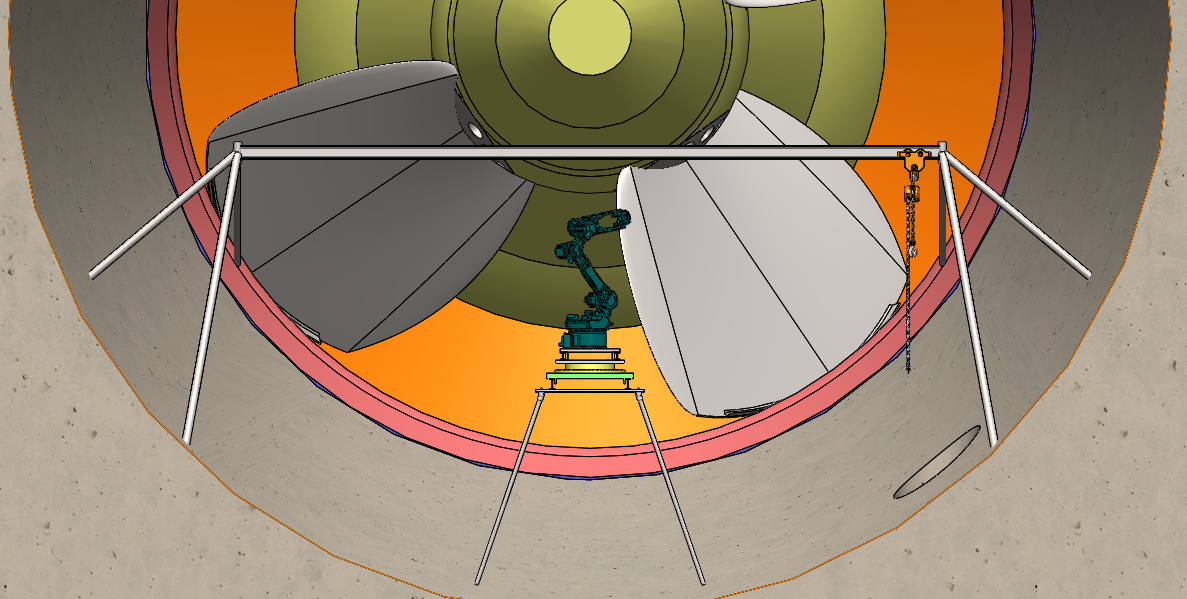
\includegraphics[width=\columnwidth]{detail/figs/bases/talha_trilho}
   \caption{Visão frontal da talha e trilho}
   \label{fig::talha_trilho}
\end{figure}

Devido aos esforços dinâmicos de operação do robô, a fixação da estutura da
base mecânica no ambiente deve ser dimensionada com cuidado. Por se
tratar de um ambiente de escoamento de fluido sob pressão, não são admitidas
modificações permanentes de infra-estrutura no interior da turbina, logo,
qualquer método de fixação utlizado deve ser removível, sem causar nenhum dano
à qualquer superfície. Em visita técnica realizada em Outrubro de $2015$ foi
testada a viabilidade de utlização de bases magnéticas para o sistema de
ancoragem e fixação. Este teste teve o objetivo de verificar a real carga limite de tração
do imã, considerando o ambiente (geometria), materiais e acabamentos
superficiais reais a que estará submetido na solução final. O resultado
detalhado do teste encontra-se no Apêndice~\ref{ape::magnetic}.

Outra opção para fixação provisória seria a soldagem da estrutura na
superfície do túnel. Esta opção segue como uma alternativa ainda para regiões
de difícil fixação da base magnética.
  
\subsection{Shutter}%TODO mudar o nome do sistema de desvio do fluxo de
% revestimento
O processo de revestimento HVOF (\textit{High Velocity Oxygen Fuel}) requer
velocidade da pistola controlada de $40~m/min$. Esta velocidade é essencial para
a qualidade do processo e deve ser mantida constante para se obter uma camada 
regular de material ao longo de toda a superfície da peça. Na solução
pesquisada demonstou-se ser inviável utilizar um robô de grande porte, devido a
limitação de acesso e ao confinamento do manipulador no ambiente. Portanto, o
manipulador  escolhido realizará o processo em regiões delimitadas da
superfície da peça e, em sua trajetória, haverá inevitavelmente mudanças de
direção, e portanto acelerações, que irão variar a velocidade da pistola.
Durante essas variações não deve-se injetar o material na peça, sendo necessário um mecanismo
autônomo para impedir o processo nestes intervalos.

A ideia inicialmente estudada foi de uma barreira (\textit{shutter}) ao fluxo na
saída da pistola.
A figura~\ref{fig::shutter_todos} ilustra a ideia para dois conceitos nas
configurações aberta e fechada. 
Nestes conceitos, uma barreira é movimentada automaticamente sempre que houver
mudança de direção da pistola, impedindo que o fluxo de material atinja a
pistola. 

\begin{figure}[h!]
   \centering
   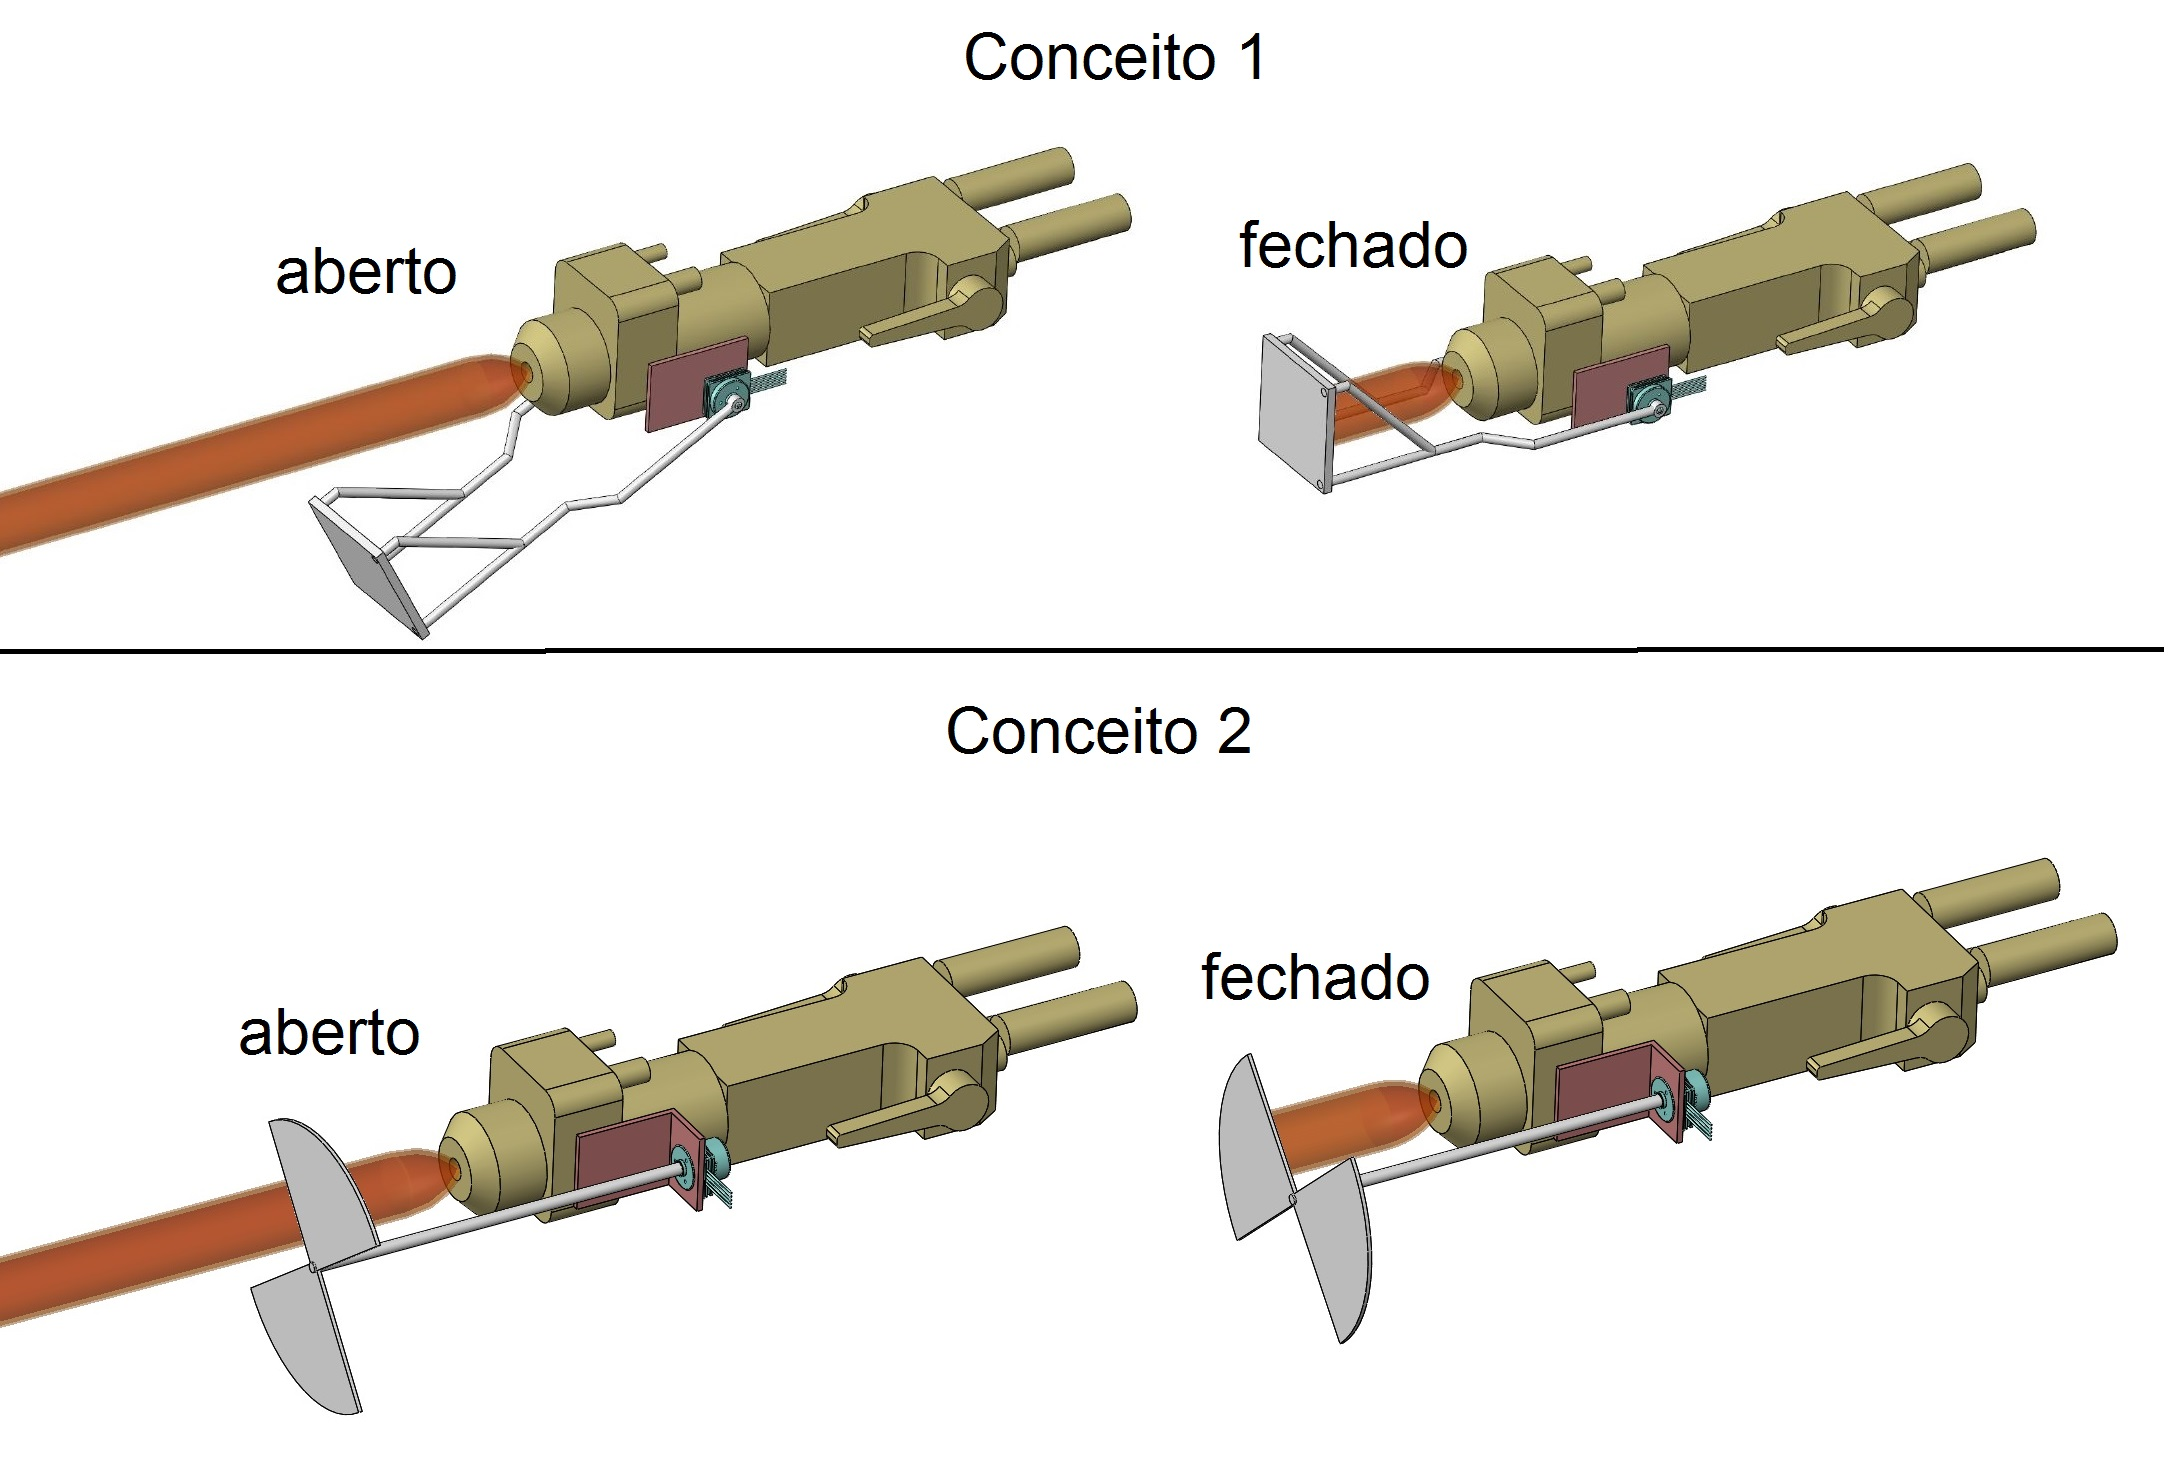
\includegraphics[width=\columnwidth]{detail/figs/shutter/shutter_todos}
   \caption{Conceitos de \textit{shutter} avaliados}
   \label{fig::shutter_todos}
\end{figure}

Algumas considerações foram levantadas para avaliar a viabilidade
desta solução, como a alta temperatura da chama, a capacidade do atuador, a
resistência mecânica da barreira e a taxa de acúmulo de material. Este conceito
foi abandonado principalmente devido ao acúmulo de material na barreira, o que
levaria a um aumento de seu peso, e por consequência momento de inércia,
alterando a dinâmica prevista, ou ainda, poderia chegar a obstruir a saída da
chama causando danos à pistola.

Outra proposta que está sendo estudada é a de modificar o fluxo da linha de
revestimento. A ideia é a inclusão de uma válvula direcional com atuação por
solenóide para desviar o fluxo do material de revestimento para um tanque ou
cilindro de retorno. Esta atuação deve ser autônoma e coordenada com a
trajetória do manipulador. A válvula seria de três vias e duas posições ($3/2$) tal que, no 
repouso, direciona-se o fluxo diretamente para a pistola e, quando
atuada, bloqueia-se o fluxo para a pistola e abre-se o fluxo para exaustão. Uma
válvula limitadora de pressão regulável seria utilizada na linha de exaustão
para igualar as diferenças de pressão entre as duas vias, minimizando efeitos
transitórios.
Outra característica opcional importante para redução dos efeitos transitórios,
como pico de pressão, é a de sobreposição aberta, ou seja, o fluxo só seria
fechado da posição inicial quando o movimento de troca estivesse completo. 
A figura~\ref{fig::circuito_hvof} apresenta o circuito do processo HVOF de forma
simplificada.

 \begin{figure}[h!]
   \centering
   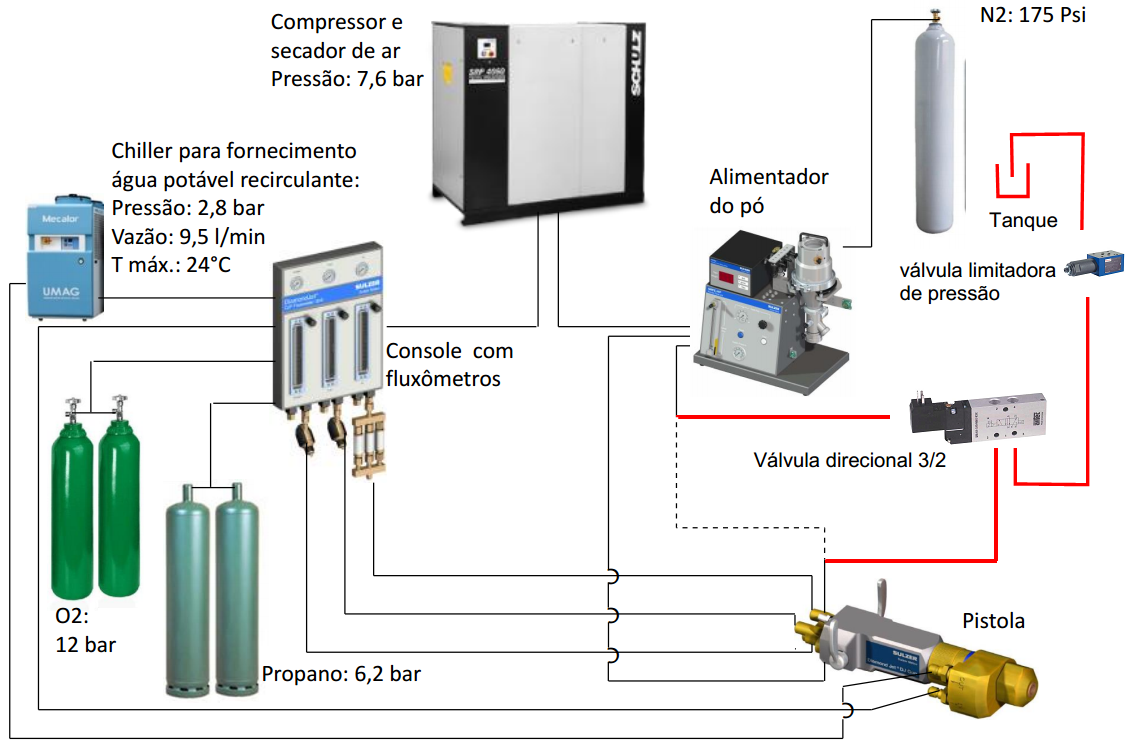
\includegraphics[width=\columnwidth]{detail/figs/shutter/Circuito_HVOF_mod}
   \caption{Circuito do processo HVOF modificado}
   \label{fig::circuito_hvof}
\end{figure}

A linha tracejada representa o circuito original, as linhas em vermelho
representam a modificação do circuito com os equipamentos adicionais indicados.

Esta é uma alternativa que tem como principal vantagem a de poder retornar a
matéria-prima do revestimento para tanque, ou seja, evita-se
o desperdício do material no ambiente. Esta matéria-prima poderia então ser
reaproveitada no processo, separando-se o gás.
 
\section{Calibração}\label{sec::calibracao}


O processo de metalização utilizado atualmente considera que a posição e
orientação da pá é fixa em relação ao robô e, uma vez, que corretamente
posicionado, o processo é executado em malha aberta. Entretanto, para qualquer
uma das soluções propostas por esse documento, não é possível assumir que nem a
posição nem a orientação do manipulador, em relação a pá a ser processada, se
manterão fixas.

Para um correto planejamento de trajetória que o manipulador deve seguir durante
a tarefa de metalização, é importante o conhecimento da transformada entre o
sistema de coordenada do manipulador e da pá a ser processada. Portanto, é
necessário utilizar algum sistema que possibilite a aquisição de informações a
respeito do ambiente e da posição relativa entre o manipulador e as pás.
\subsection{Estudo de sensores}

A utilização de um sensor de aquisição de dados espaciais não se limita somente
a loca\-lização, mas, dependendo do sistema a ser escolhido, pode também ser
útil na reconstrução do modelo do perfil hidráulico da pá, tanto do perfil ideal
quanto do estado atual da pá a ser processada (Tarefas descritas em
\ref{sec::introducao}).

Esta seção irá apresentar os segmentos de sensores que possam suprir essa
necessidade, assim como suas vantagens e limitações. 


\subsubsection{3D scanners}

3D scanners são equipamentos de alta precisão utilizados na indústria
geralmente em aplicações de metrologia, construção civil, monitoramento de
deformações, entre outras. O equipamento consiste em um feixe de laser que é
direcionado por meio de um espelho e a partir da mudança de fase do sinal
refletido é possível calcular a distância até o objeto atingido. O seu preço
esta na faixa de U\$70.000,00.

\paragraph{Estações de medição}

Esse tipo de sensor funciona a partir de um único feixe laser que é direcionado
por um espelho giratório acoplado a um motor de passo de alta resolução. O
sensor possui também uma base giratória, realizando assim um escaneamento de
$360^o$ do ambiente. Graças a sua construção, esse tipo de sensor possui uma
alta densidade de pontos e resolução, porém sua taxa de atualização não é muito
alta.

\begin{itemize}
  \item \textbf{Faro Focus X 330}
  	\begin{itemize}
  		\item Campo de visão (vertical/horizontal): $300^o$/$360^o$
  		\item Alcance: 330m
  		\item Velocidade máx. de escaneamento: 976.000pts/s
  		\item Precisão: $\pm$2mm
  		\item Peso: 5,2 kg
  		\item Tamanho: 240 x 200 x 100 mm
  		\item Vida da bateria: 4,5 horas
  		\item Temp. ambiente: $5^o$ - $40^o$ C
  		\item Preço: U\$70.000,00
	\end{itemize}
  \item \textbf{Leica P16}
  	\begin{itemize}
  		\item Campo de visão (vertical/horizontal): $270^o$/$360^o$
  		\item Alcance: 40m
  		\item Velocidade máx. de escaneamento: 1.000.000pts/s
  		\item Precisão: $\pm$3mm
  		\item Peso: 12,25 kg
  		\item Tamanho: 238 x 358 x 395 mm
  		\item Vida da bateria: 5,5 horas
  		\item Temperatura ambiente: $-20^o$ - $50^o$ C
  		\item Preço: U\$80.000,00
	\end{itemize}
   \item \textbf{Nikon MV330}
  	\begin{itemize}
  		\item Campo de visão (vertical/horizontal): $45^o$/$360^o$
  		\item Alcance: 30m
  		\item Velocidade máx. de escaneamento: 2000pts/s
  		\item Precisão: $\pm$0.5mm
  		\item Peso: \textit{não informado}
  		\item Tamanho: \textit{não informado}
  		\item Vida da bateria: \textit{não informado}
  		\item Temperatura ambiente: \textit{não informado}
  		\item Preço: U\$355.000,00
	\end{itemize}


\end{itemize}


\begin{figure}[h!]
	\centering	
	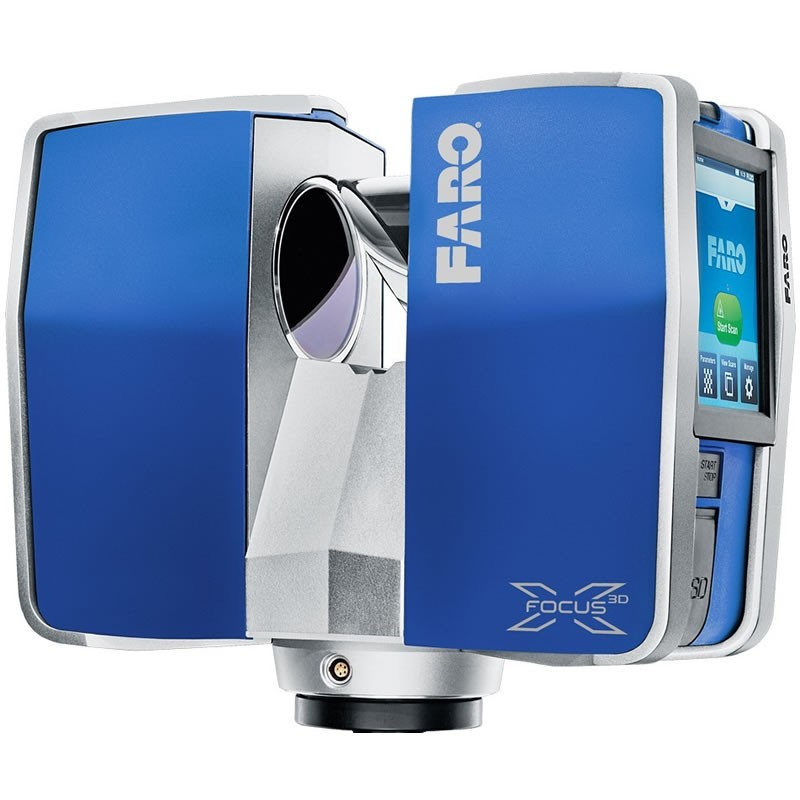
\includegraphics[width=0.5\columnwidth]{detail/figs/3dsensors/faro}
	\caption{Sensor Faro Focus X330}
    \label{fig::faro_focus}
\end{figure}

%TODO acertar figura

\paragraph{Velodyne}

A empresa Velodyne possui, atualmente, 3 modelos de 3D Lidar. Os modelos variam
basicamente no número de pares de emissores e receptores e, consequentemente, na
resolução final. Os modelos são o VLP-16, o HDL-32E e HDL-64E, com 16,32 e 64
canais respectivamente. Esse tipo de sensor possui uma alta taxa de
atualização, entretanto não possui uma alta densidade de dados. O modelo mais
utilizado é o intermediário HDL-32E.

\begin{itemize}
\item 32 pares laser/detector  
\item Campo de Visão: +10.67$^o$ to -30.67$^o$ (vertical)
\item Rotação de $360^o$
\item Alcance - 1m - 100m 
\item 10 Hz frame rate (selecionável 5-20Hz)
\item Temperatura de Operação $-10^o$ to $+60^o$ C
\item Acurácia: $<$2 cm
\item Resolução Angular (vertical) 1.33$^o$
\item Peso: HDL-32E = 1kg; Cabos = 0.3kg
\item Tamanho: 15cm altura x 8.6cm diâmetro
\item Proteção: IP67
\item Correção de orientação (internal MEMS acelerometros and gyros)
\item Preço: U\$30.000,00
\end{itemize}

\begin{figure}[h!]
   \centering
   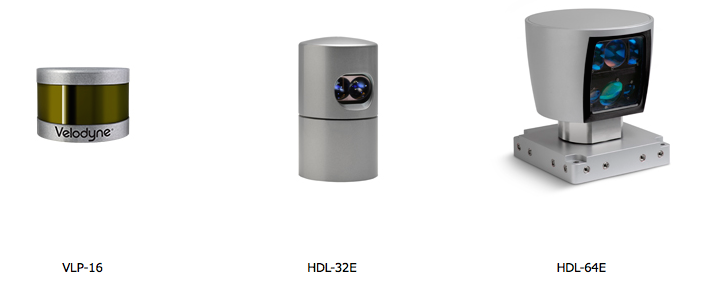
\includegraphics[width=\columnwidth]{detail/figs/3dsensors/velodyne}
   \caption{Velodyne Models}
   \label{fig::velodyne_models}
\end{figure}

\paragraph{Forecast 3D Laser System}


O sensor Forecast 3D consiste em um senor 2D laser da SICK, modelo LMS 151 ou
511, acoplado a uma unidade $pan-tilt$. O seu preço esta na faixa de
U\$37.000,00.


\begin{figure}[h!]
   \centering
   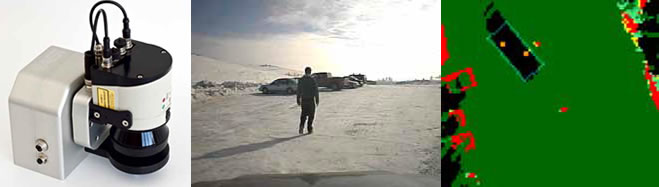
\includegraphics[width=\columnwidth]{detail/figs/3dsensors/forecast}
   \caption{Forecast 3D Laser System}
   \label{fig::forecast}
\end{figure}

\subsubsection{ToF Cameras}

Conhecidas como Time-of-Flight Cameras, são dispositivos compostos por apenas
uma câmera, não necessitando de uma configuração estéreo para triangularização
de imagens. Esse tipo de dispositivo utiliza uma fonte infra-vermelho interna e de
forma análoga aos dispositivos laser, calcula a distância a partir da diferença
de fase do sinal refletido. Entretanto, essa tecnologia possibilita o cálculo
simultâneo das distâncias de cada objeto na região iluminada pela fonte IR,
mesmo que com resoluções limitadas.

\paragraph{Mesa Imaging SwissRanger SR4000}


\begin{itemize}
  \item Alcance para detecção: 0.1 - 10.0 m
  \item Alcance calibrado: 0.8 - 8.0 m
  \item Drift com a temperatura (T) - $\leq$ 1.5 mm/$^o$C (max.) - For 10$^o$C
  $\leq$ T $\leq$ 50$^o$C
  \item Tamanho: 65 x 65 x 76 mm
  \item Peso: 510 g
\end{itemize}

\begin{figure}[h!]
   \centering
   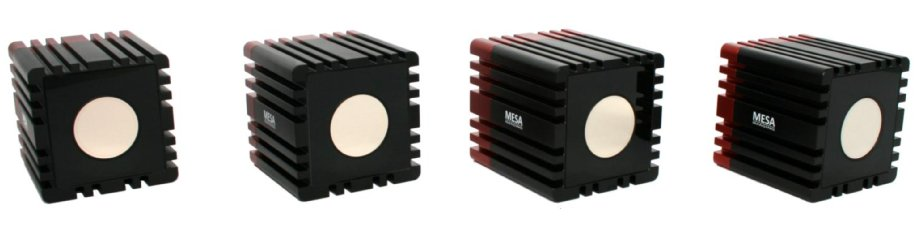
\includegraphics[width=\columnwidth]{detail/figs/3dsensors/mesa2}
   \caption{Mesa Imaging SwissRanger SR4000}
   \label{fig::mesa}
\end{figure}

\paragraph{Sentis M100 / Argos 3D - P100}

\begin{itemize}
  \item Medidas de distância e vídeo em tons de cinza
  \item Resolução: 160 x 120 pixels
  \item 40 - 160 fps
  \item Alcance: $>$3m  (extensível até 10m indoor)
  \item Campo de Visão: $90^o$
  \item Tamanho: 75 x 57 x 26 mm
  \item Peso:  	140 g  
\end{itemize}

\begin{figure}[h!]
   \centering
   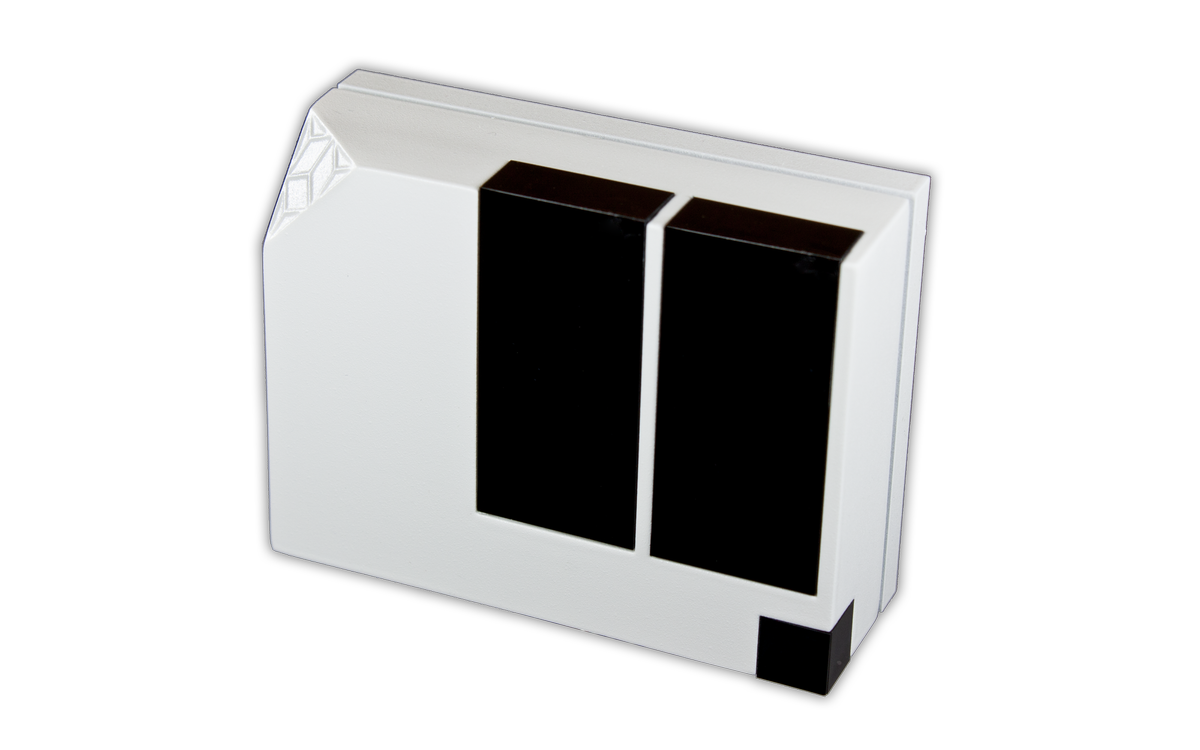
\includegraphics[width=0.6\columnwidth]{detail/figs/3dsensors/argos3dp100}
   \caption{Sensor Argos 3D - P100}
   \label{fig::forecast}
\end{figure}

\subsubsection{Câmeras de Luz Estruturada}

Estes sensores constituem de uma fonte emissora de infra-vermelho e um receptor.
Um padrão é projetado na cena a ser reconstruida e a partir da distorção desse
padrão é possível o cálculo de distâncias. 

%TODO exemplos dos sensores de luz estruturada
%TODO Pros e cons

%TODO ELAEL - decidir se abre uma subseção d eaplicações ou coloca um exemplo de
% aplicação em cada componente - utilizar o seu material do SOTA em 3D sensors. 

\begin{center}
\begin{tabular*}{\columnwidth}{l @{\extracolsep{\fill}} cc}
\hline
{\bf Características}           & {\bf
\begin{tabular}[x]{@{}c@{}}Luz\\Estruturada\end{tabular}}                       
& {\bf ToF}                                                  \\ \hline {\bf Complexidade de Software}  & Média                                                      & \cellcolor[HTML]{92D050}{\color[HTML]{000000} {\bf Baixa}} \\
{\bf Custo Material}            & \cellcolor[HTML]{FE0000}{\color[HTML]{FFFFFF} {\bf Alto}}  & Médio                                                      \\
{\bf Tamanho}                   & Grande                                                     & \cellcolor[HTML]{92D050}{\bf Pequeno}                      \\
{\bf Tempo de Resposta}         & \cellcolor[HTML]{FE0000}{\color[HTML]{FFFFFF} {\bf Alto}}  & \cellcolor[HTML]{92D050}{\bf Baixo}                        \\
{\bf Acurácia da Profundidade}  & \cellcolor[HTML]{92D050}{\bf Alta}                         & Média                                                      \\
{\bf Qualidade com Pouca Luz}  & \cellcolor[HTML]{92D050}{\bf Boa}                          & \cellcolor[HTML]{92D050}{\bf Boa}                          \\
{\bf Qualidade com Muita Luz} & \cellcolor[HTML]{FE0000}{\color[HTML]{FFFFFF}
{\bf Fraca}} & \cellcolor[HTML]{92D050}{\bf Boa}                          \\
{\bf Consumo de Energia}        & Médio                                                      & \cellcolor[HTML]{92CDDC}{\bf Escalavel}                    \\
{\bf Alcance}                   & \cellcolor[HTML]{92CDDC}{\bf Escalavel}                    & \cellcolor[HTML]{92CDDC}{\bf Escalavel}                    \\ \hline
\end{tabular*}
\captionof{table}{Comparativo Luz Estruturada vs ToF. Fonte: \citep{larrylitof}}
%\caption{Dados principais do processo de metalização HVOF}
\label{tab::estructvstof}
\end{center}

\subsection{Conclusão}

As restrições apresentadas pelo problema de calibração, dentro do ambiente da
turbina, impõem um conjunto de requisitos mínimos que o sensor deve apresentar:

\begin{itemize}
  \item Alta resolução
  \item Portabilidade
  \item Alcance suficiente ($>$20m)
  \item Resistir as condições de temperatura e umidade 
\end{itemize}

Além desses requisitos, é desejável também que o sensor tenha alimentação
idependente e que sua velocidade de escaneamento não seja um fator limitante
para a eficiên\-cia do processo.

A classe de sensores que atende todas essas condições é a das Estações de
medição, com exceção do sensor Nikon MV 330 que não possui a portabilidade
necessária para a solução proposta, além de ter um preço muito maior que de seus
concorrentes.

O sensor Faro Focus X330, além de satisfazer os requisitos mínimos, é o que
possui menor preço e, por isso, foi escolhido como o o sensor a ser utilizado na
calibração do sistema e reponsável por colher os dados espacias do ambiente da
turbina e do robô. 

Entretanto, pelas especificações do sistema não foi possível garantir a perfeita
opera\-ção do sensor nas condições de alta umidade apresentada no interior da
turbina. O dipositivo opera com um sistema de lentes e lasers e, caso apresente
condensação em um desses componentes, o resultado final de sensoriamento pode
ser prejudicado. Devido a este fato, foi realizado uma bateria de testes na
Usina Jirau, no interior de uma turbina, afim de confirmar a viabilidade
técnica desse sensor.

O teste realizado constituiu na utlização de quatro esferas reflexivas,
representadas na figura \ref{fig::esferas}, distribuidas pelo ambiente da
turbina.
Em seguida, foram realizadas 4 coletas de dados, sendo 3 delas à jusante do
rotor e uma entre as pás do rotor e o distribuidor. Com a nuvem de pontos
coletada, foi possível utilizar a assinatura única gerada pelas esferas para
alinhar todos os conjuntos de dados em uma única imagem 3D.

\begin{figure}[h!]
\centering
	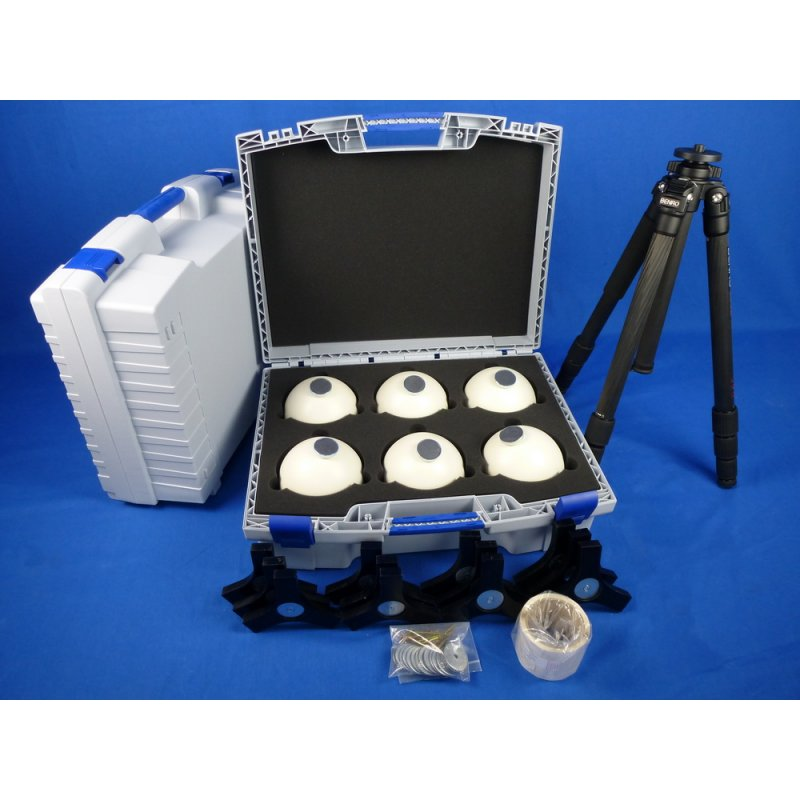
\includegraphics[width=0.7\columnwidth]{detail/figs/3dsensors/kit}
	\caption{Conjunto de esferas reflexivas e tripé}
	\label{fig::esferas}
\end{figure}

A figura \ref{fig::turbina_faro} representa a vista frontal da imagem gerada e, por sua
vez, a figura \ref{fig::turbina_cad} representa uma reconstrução 3D gerada a
partir da nuvem de pontos coletas e utilizando o software proprietário do
fornecedor do sensor. 

\begin{figure}[h!]
\centering
	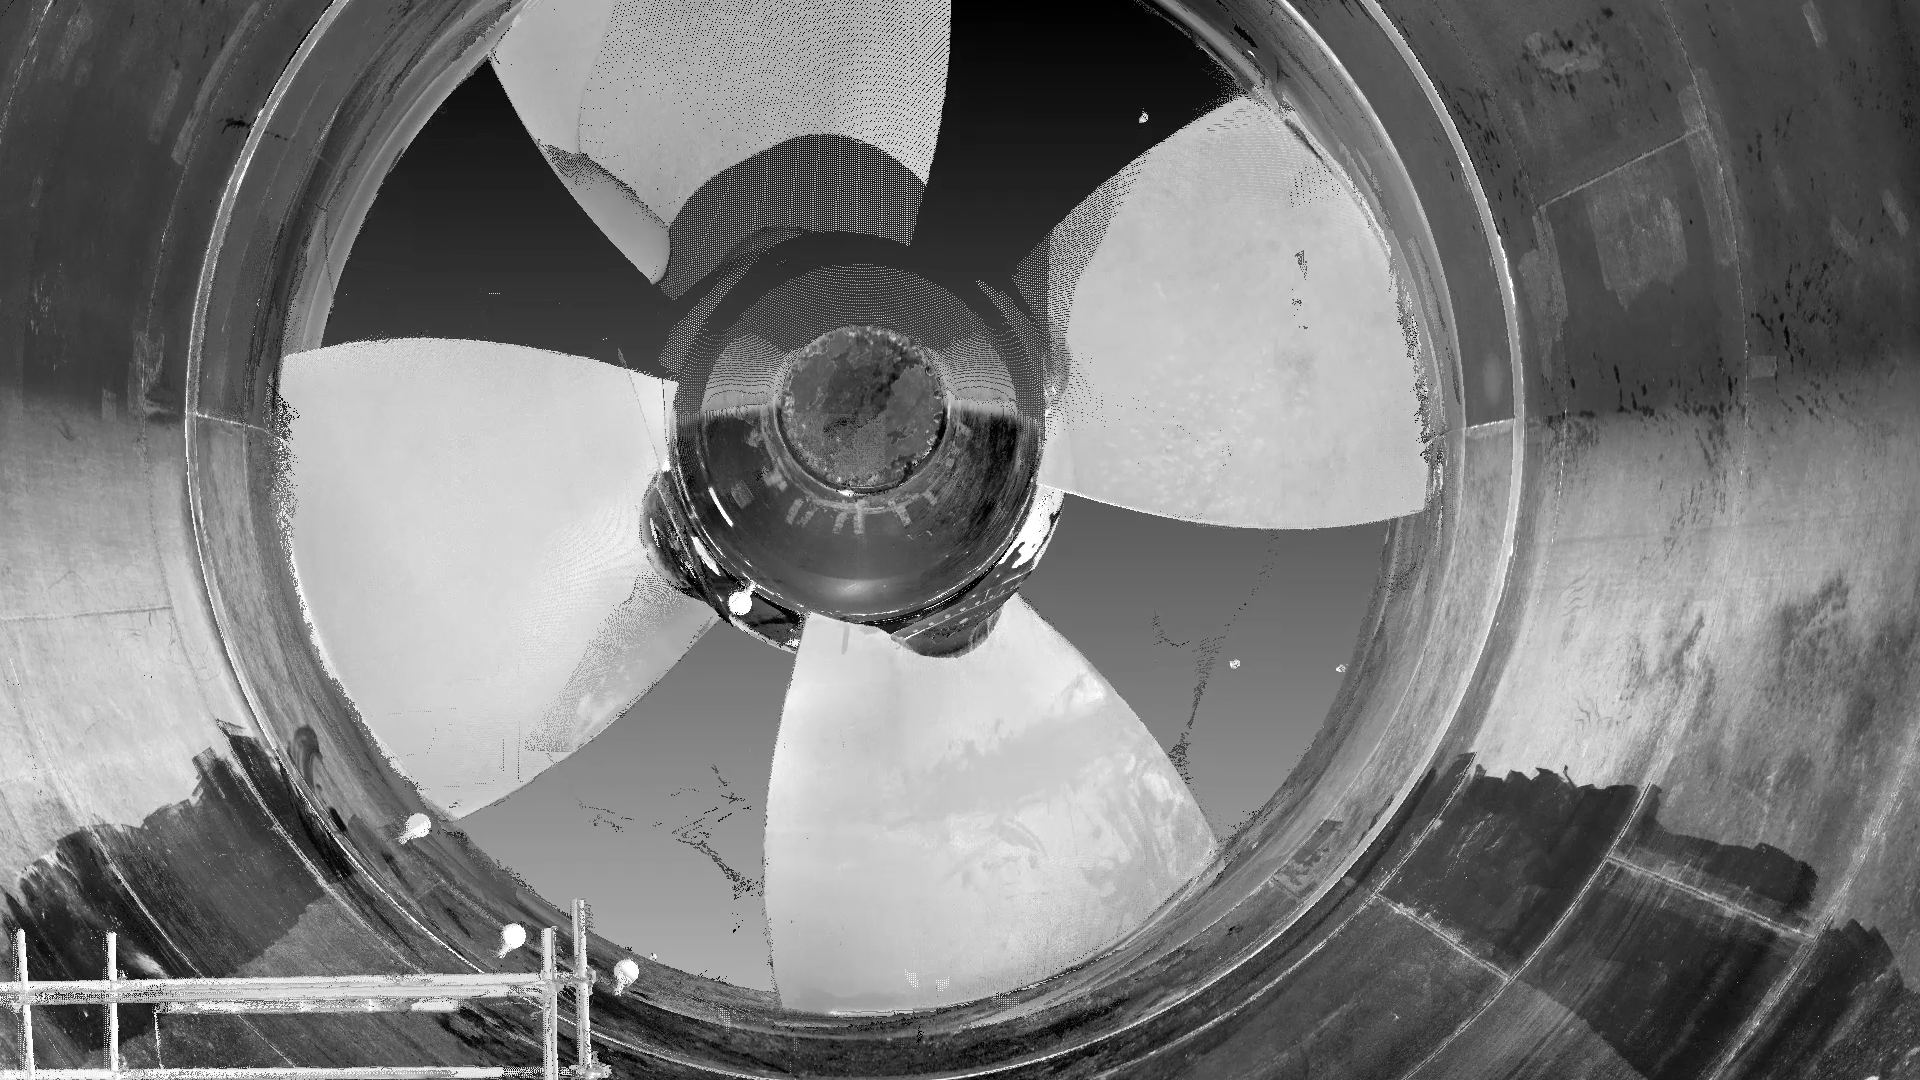
\includegraphics[width=0.8\columnwidth]{detail/figs/3dsensors/recorte_video}
	\caption{Vista frontal da imagem gerada a partir dados adquiridos durante o
	teste na UHE Jirau.}
	\label{fig::turbina_faro}
\end{figure}

\begin{figure}[h!]
\centering
	\includegraphics[width=0.8\columnwidth]{detail/figs/3dsensors/Pa_Real_Render_04}
	\caption{Reconstrução em CAD da pá com os dados do teste.}
	\label{fig::turbina_cad}
\end{figure}

A partir dos resultados gerados durante os testes foi comprovada que o sensor é
capaz de operar nas condições extremas impostas pela turbina e com um nível de
ruído aceitável para a aplicação em questão. 


\subsubsection{Medidor de distância a Laser}

Durante o processo de metalização o 3D scanner estará desligado, pois o tempo de
varedura não o torna prático para obter informações em tempo real. Assim o
sistema estaria funcionando em \textit{loop} aberto, o que gera receios com
relação à segurança. A fim de evitar tais riscos é desejável alguma
realimentação para o sistema sobre sua posição. Essa realimentação será
realizada pelo uso de um medidor de distância a Laser, a ser posicionado próximo
à pistola de metalização, com o intuito de aferir a distância da pistola até a
pá em tempo real.

\begin{figure}[h!]
\centering
	\includegraphics[width=0.9\columnwidth]{detail/figs/3dsensors/senso_laser_pistola}
	\caption{Ilustração da posição do medidor de distância, em cinza, na pistola de
	metalização.}
	\label{fig::laser}
\end{figure}


Para a escolha de medidor compatível foram analisadas as seguintes variáveis:

\paragraph{Temperatura}
A temperatura da superfície pode influenciar na precisão do sensor devido à
radiação de corpo negro. Caso essa radiação térmica atinja níveis relevantes na
faixa de frequência do Laser utilizado ocorre degradação da qualidade de
reposta do sensor. Análises de campo identificaram que, apesar da alta
temperatura da chama de metalização, a pá da turbina não chega a emitir níveis
preocupantes de radiação na faixa do vermelho ($670 nm$), onde operam os Lasers
padrões. Para casos de exceção existem Laser que trabalham em regiões do
azul/violeta.

Por outro lado a temperatura do ambiente também influencia o sensor, que não
costuma ter alta resistência à temperatura, ficando algo em torno do $50^oC$.
Para evitar que o calor da chama seja recebido diretamente pelo sensor,
aumentando a temperatura ambiente na região, ele deve ser posicionado na pistola
com uma distância de segurança da chama (figura \ref{fig::laser}).

\paragraph{Distância de operação}
A metalização ocorre com a pistola entre 23cm e 24cm de distância da pá. Somado
a isso temos a distância do sensor à chama para então sabermos a distância da
pá ao sensor. Considerando que a pistola possui em torno de 30cm de comprimento,
a faixa de operação de distâncias do sensor deverá incluir 40-50cm. Para termos
essa região no centro da faixa de operação, ela deverá iniciar em 20-25cm e
trabalhar até 80-100cm.

\paragraph{Poeira e Umidade}
A alta umidade ambiente dentro do aro câmara, e em todo circuito hidráulico,
impõe mais um requisto sobre o equipamento. Além disso, o pó residual da
aplicação da metalização pode ser danoso ao sensor. Um isolamento apropriado
para o sensor pode ser encontrado segundo a padronização IP69K.

\paragraph{Precisão}
Como a tolerância está na ordem de milímetros ( a distância do sensor à pá deve
se manter em uma faixa de $\pm 5mm $ entre 23cm e 24cm ), logo é desejável que o
sensor possua precisão de $1mm$ ou menor.

\paragraph{Peso}
Considerando a carga máxima no punho do robô de 10kg, e a massa da pistola de
8,5kg e aplicando as restrições dinâmicas ( para manter a velocidade
desejada em todos os pontos ) conclui-se que o medido deve ter uma massa
inferior a 1kg.



%\subsection{Estudo de técnicas de reconhecimento} 

As informações de distância recebidas pelos sensores descritos na seção
anterior podem ser armazenados como uma estrutura de dados chamada nuvem de
pontos, isto é, uma representação tridimensional do espaço cartesiano, na qual cada distância medida pelos
sensores a partir de sua origem representa uma coordenada x y z.
Entretanto, essa representação não é capaz de diferenciar, ou classificar, os
limites de cada objeto presente na cena, ou seja, não é possível determinar
\textit{a priori} qual conjunto de pontos pertence a cada elemento que se deseja
identificar para realizar a calibração.

A identificação de cada conjunto, ou \textit{cluster}, de pontos é importante
para que a posição e orientação de cada objeto de interesse seja determinada e,
assim a transformação do sistema de coordenadas entre cada objeto seja
calculada. Esse processo necessita, então, do estudo e implementação de
algoritmos para a análise da nuvem de pontos, identificação dos elementos
necessários, extração de suas respectivas posições e, finalmente, cálculo da
transformação entre as posições. 

Dependendo das características de cada objeto a ser identificado e da
possibilidade de implementação de uma estrutura de apoio para facilitar a sua
identificação, podem ser utilizados diferentes métodos e estratégias de
identificação e localização, que serão exploradas a seguir.

\subsubsection{Reconhecimento do Robô}

O Robô é uma estrutura que a idenficação pode ser facilitada pelo uso de
padrões de fácil reconhecimento (como esferas e padrões de xadrez, figuras
\ref{fig::sphere_rec} e \ref{fig::checkerboard_rec} ), pois alterações na base
do robô não ocasionam problemas para o funcionamento do sistema.


\begin{figure}[h!]
   \centering
   \includegraphics[width=0.95\columnwidth]{detail/figs/localizacao/sphere_rec}
   \caption{Exemplo de esfera utilizada para reconhecimento. Fonte:
   http://shop.talwin.net/}
   \label{fig::sphere_rec}
\end{figure}



\begin{figure}[h!]
   \centering
   \includegraphics[width=0.95\columnwidth]{detail/figs/localizacao/checkerboard_rec}
   \caption{Exemplo de padrão de xadrez utilizado para renhecimento.\\ Fonte:
   http://stereomorph.blogspot.com.br/}
   \label{fig::checkerboard_rec}
\end{figure}


Devido a baixa iluminação ambiente dentro do circui\-to da tubina, a opção
mais simples é o uso de nu\-vem de pontos sem identificação de cor. Ou seja, o
reconhecimento se dará apenas pelo formato. Isso restringe o uso de padrões de
xadrez e o foco se voltará, então, para o uso de formatos geométricos. Em
especial o mais simples objeto de três dimensões: a esfera.

O reconhecimento de formas geométricas simples em três dimensões é um assunto
já razoavelmente explorado na literatura. Dentre eles pode-se destacar 2
métodos: RANSAC e Hough Transform.

\paragraph{RANSAC}
O método RANSAC (acrônimo para ``RANdom SAmple Consensus", \textit{consenso por
amostragem aleatória} em tradução livre) é um método iterativo que tem como
premissa a presença de \textit{outliers} (elementos fora do corpo principal) na
amostra e objetiva a identificação dos parâmetros matemáticos que descrevem o
objeto geométrico em questão \cite{ransac}. É o método
disponível na amplamente utilizada biblioteca de processamento de nuvem de pontos ``PCL''. 

Esse método consiste na seleção aleatória de pontos para serem considerados como
partes integrantes do corpo principal (no caso, uma esfera), a partir desses os
parâmetros da esfera são calculados (comumente, os valores x, y e z do centro
da esfera e seu raio). Então os demais pontos são julgados como fazendo parte ou
não da esfera de acordo com esses parâmetros. O modelo é avaliado como bem estimado se uma quantidade razoável de pontos são considerados
como pertencentes à esfera. Se for visto como bem estimado, os parâmetros são
então reestimado levando em conta de todos os pontos que foram considerados como
pertencentes à esfera. O erro do modelo é inferido a partir dos pontos que foram
considerados como fazendo parte da esfera e uma esfera reconstruída pelos
parâmetros calculados. O processo então é repetido um número artrário de vezes,
e se mantém armazenado o modelo que obteve menor erro.

Um dos principais pontos negativos do RANSAC é que ele tem como premissa a
presença de apenas um corpo principal, ou seja, apenas uma esfera. Isso implica
em um tratamento especial quando temos mais de uma esfera no ambiente.

\begin{figure}[h!]
   \centering
   \includegraphics[width=0.95\columnwidth]{detail/figs/localizacao/ransac}
   \caption{Exemplo de reconhecimento de uma linha em 2 dimensões usando
   RANSAC. (Fonte: \cite{ransac})}
   \label{fig::ransac}
\end{figure}
 
 \paragraph{Transformada de Hough 3D}
Anos de pesquisa em reconhecimento de objetos geométricos de duas dimensões
levaram ao desenvolvimento e aprimoramento de técnicas basedas em ``Transformada
de Hough''. Essas técnicas tem sido recentemente adaptadas para o universo de
três dimensões (ver \cite{hough2014}) e adequadamente chamadas de Transformada
de Hough 3D.

O método consiste em tranformar cada ponto do espaço 3D em uma variedade
mergulhada no espaço quadridimensional dos parâmetros da esfera ( x, y e z do
centro mais r do raio). A variedade se identifica com todas as possiveis esferas
que contém aquele ponto. O espaço de parâmetros é então restrito dentro de
certos limites e quantizado por razões de implementação (os recursos
computacionais são finitos). É definido então um acumulador, basicamente uma
função que conta quantas variedade interceptam determinada região discretizada
do espaço de parâmetros. Um algorítmo de reconhecimento de picos é aplicado
sobre o espaço de parâmetros (com as varidade já mergulhadas nele) para detectar
qual o conjunto de parâmetros que está melhor descrevendo um maior número de
pontos. O algorítmo pode ser utilizado para reconhecer mais de um pico e, assim,
identificar a presença de mais de uma esfera na nuvem de pontos (exemplo na
figura \ref{fig::hough}).

A dificuldade no uso do método é seu custo computacional, mas existem soluções
que exploram amostragens estatísticas para reduzir o custo computacional.

\begin{figure}[h!]
   \centering
   \includegraphics[width=0.95\columnwidth]{detail/figs/localizacao/hough}
   \caption{Exemplo de reconhecimento de duas linhas em 2 dimensões usando
   Transformada de Hough. Na esquerda estão pontos que compõem as duas retas, na
   direita uma sobreposição das variedades referentes a cada ponto das retas
   (mergulhadas em um espaço paramétrico bidimensional). Os pontos mais
   brilhantes refletem os picos referentes aos parâmetros que melhor descrevem as duas retas. (Fonte: 
   \url{https://en.wikipedia.org/wiki/Hough_transform})}
   \label{fig::hough}
\end{figure}

Tendo conhecimento da posição de quatro esferas, pelo uso de um dos métodos
descritos acima, é possivel unicamente identificar a posição de um corpo preso a
elas. Em outras palavras, consegue-se a transformada entre origem do sistema de
coordenadas (tipicamente no sensor) e o robô. Para descobrir a trasnformada
entre o robô e a pá (posição relativa entre eles) falta identificar a
transformada entre a origem e a pá, esse caso será explorado na próxima seção a
seguir.

\subsubsection{Reconhecimento da Pá} 

Para a identificação e localização das pás das turbinas não é possível a
utilização de nenhum artifício de apoio que facilite o processamento da nuvem de
pontos, pois a instalação de qualquer um desses aparatos não pode ter precisão
garantida nas operações de campo. Uma instalação de um elemento de apoio em
pontos precisos da pá necessitaria também de calibração para cada utilização, retirando assim
o propósito do método. 

Portanto, para a localização das pás da turbina é
necessário explorar as características espaciais intrínsecas à superfície do
próprio objeto e identificá-las na nuvem de pontos do ambiente. O objetivo
principal nessa etapa do processo é, então, identificar um conjunto mínimo de
características do objeto que o represente unicamente com um baixo grau
de ambiguidade e sem exigir muito esforço computacional. 

A escolha do tipo de característica a se usar é uma decisão fundamental para a
eficiência do processo e tem sido alvo de estudos na literatura para a análise
e reconhecimento de imagens 2D, como imagens RGB de câmeras e mais recentemente
também para imagens 3D. 

Uma boa representação de \textit{point feature} deve ser capaz de capturar as
mesmas características locais da superfície na presença de:

\begin{itemize}
  \item \textbf{Transformadas} -  rotações e translações 3D nos dados não devem
  influenciar a estimação dos descriptors;
  \item \textbf{Variações na densidade de amostragem} - em princípio, uma de
  superfície amostrada mais ou menos densamente deve ter a mesma assinatura característica do vetor
  \item \textbf{Ruído}
\end{itemize}

O reconhecimento de objetos em aplicações robóticas também vem recebido
grande atenção, principamente com o crescimento da robótica móvel e em ambientes
não estruturados, onde é necessário identificar e localizar os objetos a serem
manipulados em cada tarefa. O problema é enfrentado basicamente utilizando-se
duas abordagens: analisar os dados 3D ou realizar algum tipo de processamento e
projeção para se trabalhar com imagens 2D e utilizar as técnicas mais maduras
desse tipo de imagem.

Nesta última categoria, a técnica
mais usada consiste em converter as informações tridimensionais em \textit{Range
Images}, na qual é realizada uma projeção a partir de um ponto de vista (geralmente o do sensor) e utiliza escala
de cores ou cinza para representar a distância, ou seja, quanto mais escuro o
objeto na imagem, mais longe ele se encontra. É importante reassaltar que esse
tipo de método introduz perdas de informação ao se realizar projeções e é
sensível à escolha do ponto de vista escolhido. 
%Em \cite{Bayramoglu2010} são
%utilizados descritores SIFT, ou \textit{Scale-Invariant Feature Transform},  
%como características a serem identificadas na imagem. \textit{Local Feature
%Histograms} são utilizados em \cite{Hetzel2001} e por sua vez \cite{Chen2007}
%optou por utilizar \textit{Local surface patches}. 
A escolha do descritor a ser
utilizado depende da aplicação e deve ser estudada a melhor opção para a nossa
solução, assim que tivermos dados aquisitados pelo sensor. Aplicações
semelhantes envolvendo identificação de objetos no ambiente tridimensional, mas
sem localizá-los, e utilizando diferentes descritores podem ser encotradas em
\cite{Bayramoglu2010,Hetzel2001,Chen2007}. Uma comparação dos descritores
utilizados para reconhecimento de objetos 2D e 3D pode ser encontrado em \cite{Zaharia2004, Weber2014}.

Após o reconhecimento do objeto, é necessário identificar a sua posição.
Em \cite{Steder2009}, o alinhamento é realizado utilizando-se a própria
\textit{Range Image} e a informação de profundidade presente na mesma. Por outro
lado, em \cite{Nuchter2005} a região onde o objeto identificado está presente é
selecionada e, por meio de \textit{raycasting} o conjunto de pontos da nuvem
pertecentes à região identificada na \textit{Range Image} é reprojetado. Após
essa segmentação, é utilizado um algoritmo de alinhamento como o ICP.

O primeiro passo para tornar possível a localização da pá é a aquisição de seus
dados espacias e a criação de uma nuvem de pontos que a represente. A
figura \ref{fig::pa_pcd} ilustra uma nuvem de pontos representando uma pá de uma das
turbinas da usina de Jirau, esse modelo foi construído utilizando-se os dados
aquisitados durante a viagem de campo e teste de sensibilidade do sensor Faro
Focus X330, como citado anteriormente. É importante ressaltar que o
modelo deve representar, se possível, todas as características pertinentes do objeto de interesse. Nesse
sentido, se faz necessário a criação de um modelo para cada tipo de pá que
deverá ser processada, ou seja pás com diferentes perfis hidráulicos possuem
modelos diferentes.


\begin{figure}[h!]
   \centering
   \includegraphics[width=0.95\columnwidth]{detail/figs/localizacao/pa_pcd}
   \caption{Modelo da pá em nuvem de pontos}
   \label{fig::pa_pcd}
\end{figure}

A partir do modelo, é necessário a extração de seus pontos chaves e descritores.
A figura \ref{fig::pa_key} ilustra descritores do tipo SHOT, identificados no modelo de referência da pá. Para a nossa aplicação, não é
necessário, a princípio, o reconhecimento do objeto em questão, apenas a sua
localização e orientação no espaço tridimensional. A possibilidade de inserir no
sistema a informação de qual modelo de pá deve ser procurado, simplifica o
algoritmo e o torna menos suscetível a erros, uma vez que não é necessário
avaliar qual o modelo mais próximo das medições atuais e ainda é possível 
utilizar essa informação para fornecer uma avalição da similaridade do modelo
com os dados reais aquisitados.

\begin{figure}[h!]
   \centering
   \includegraphics[width=0.95\columnwidth]{detail/figs/localizacao/pa_key}
   \caption{Pontos de interesses com descritores associados no modelo da pá}
   \label{fig::pa_key}
\end{figure}

Uma vez que os pontos de interesse do modelo e seus descritores são extraídos, é
possível armazená-los para evitar o seu processamento  durante cada nova
calibração. Utilizando-se a estratérgia de
\textit{Correspondence Grouping} e o algoritmo \textit{Hough Voting}
\cite{Tombari2010a}, a nuvem de pontos aquisitada em campo terá também seus
pontos de interesse extraídos e um descritor associado para cada ponto. A
seguir, os descritores de ambas as nuvens, cena e modelo, são comparados afim de
se encontrar correpondentes em cada conjunto. Se um número suficiente de
correspondências é encontrado, o objeto é então detectado e localizado na
imagem. É importante ressaltar que essa técnica pode gerar falsos positivos. A
figura \ref{fig::correspondence} ilustra a implementação do algoritmo com 
dados sintéticos de uma cena, utilizando-se porém o modelo real da pá. O modelo
da pá está representado em amarelo, a pá identificada na cena em vermelho e as correspondências
conectadas pelas setas verdes.
Como próximos passos é necessário a utilização de dados reais para validação do
algoritmo e também a utilização de diferentes descritores, uma vez que apenas os
descritores do tipo SHOT foram testados.

\begin{figure}[h!]
   \centering
   \includegraphics[width=0.99\columnwidth]{detail/figs/localizacao/correspondence}
   \caption{Identificação e localização de uma pá utilizando
   \textit{Correspondence Grouping}}
   \label{fig::correspondence}
\end{figure}







 \section{Interface de Usuários}\label{sec::interface} 

A interface gráfica do usuário permite a interação com o manipulador para a
executar as tarefas inspeção e metalização das pás in Situ. O objetivo é de facilitar a usabilidade do software dando
visibilidade aos dispositivos do sistema e monitorando o processo de metalização das pás.
O estudo de viabilidade técnica prevê seu detalhamento até seu design
conceitual, uma vez que seu desenvolvimento efetivo acontecerá posteriormente na
fase de execução do projeto EMMA.


\subsection{Pesquisa de usuários}
A pesquisa de usuário identifica todos os atores possíveis no contexto de uso do
software em questão, assim como coleta dados a respeito de seus possíveis usuários com o intuito de 
aprender sobre suas características, necessidades e preferências. Seu objtivo é
de elaborar arquétipos que sirvam como referência na tomada de decisões e na
arquitetura e design do sistema, bem como auxiliar nos requisitos funcionais e
não funcionais.


\subsection{Análise de Tarefas}
A análise de tarefas ocorre de forma simultânea a pesquisa de usuários, podendo
ser aplicado a uma variedade de técnicas para identificar e compreender a estrutura, o fluxo, 
e os atributos de tarefas executadas na metalização das pás. Seu objetivo é de
identificar as ações e processos cognitivos necessários que o usuário complete
uma tarefa ou atinja um objetivo particular. A partir desta análise de tarefas é
possível projetar e atribuir atividades de forma adequada dentro do novo sistema.
Para realizar a metalizaçào das pás in Situ o softeware do robô EMMA vai
realizar 3 tarefas distintas: calibração, planejamento de trajetória e
metalização.


\subsubsection{Calibração}
A etapa de calibração é efetuada toda vez que o robô precisa ser
posicionado ou reposicionado no ambiente do aro câmera. O objetivo é de
reconhecer no ambiente confinado todos os elementos que fazem parte da
operação. Através de um sensor laser é obtida uma nuvem de pontos que
posteriormente é analisada e fornece as posições do manipulador em relaçào a pá
e ao trilho mecânico. A partir desses dados é opossível realizar o planejar a
trajetória do robô.


\subsubsection{Planejamento de Trajetória}
Planejamento de trajetória define como o robô irá executar a aplicação de
revestimento nas pás. A partir das posições do robô em relaçào a pá são geradas
trajetórias que o efetuador irá percorrer para realizar o revestimento em toda a
superfície da pá. Cada configuração do manipulador se relaciona com uma lista de
ângulos das juntas do robô. A aplicação de metalizaçào é dividida em
etapas, para cada uma delas são geradas n configurações gerando assim uma matriz de
ângulo dessas juntas.


\subsubsection{Metalização}
A etapa de matalização conclui o processo de reparo e manutenção das pás pa
partir da aplicação de revestimento metálico. Como definido no \textit{Estudo do
conceito para metodologia e revestimento robótico de turbinas In situ}


\subsection{Casos de Uso}
Casos de uso descreve os cenários e usuários presentes nas atividades do robô.
Desta forma é possível viazualizar funcionalidades do sistema do ponto de vista
do usuário e de auxiliar na comunicação entre desenvolvedores e
clientes.

\subsection{Design Conceitual}
Design conceitual corresponde a um protótipo baseado na pesquisa de usuários,
análise de tarefas e casos de uso. É elaborado um desenho de estrutura, mais
conhecido como 'wireframe' onde se descreve as funcionalidades e posicionamento
de dispositivos. A partir são elaborados os primeiros testes de interação para
verificar seu funcionamento.

\subsection{Estrutura de Testes de Usabilidade}
Em um primeiro momento é preciso testar a estrutura do teste por meio de
observação dos usuários. Ao verificar se os testes são capazes de prover as
informações necessárias, é definido como o teste de usabilidade será aplicado.
Nesse contexto é de suma importância que todas vezes que o teste ocorra, seja
aplicado a um usuário diferente. O objetivo é que este não tenha em mente o
teste anterior a fim de garantir sua eficiência.








\section{Conclusão e trabalhos futuros}\label{sec:conclusions}

Este documento teve como objetivo: fazer uma análise das restrições do processo
de revestimento por aspersão térmica; caracterizar o ambiente de trabalho onde o
processo será realizado; fazer um estudo detalhado do estado da arte que
visaram solucionar um problema semelhante ou possuíam tecnologias que
poderiam ser utilizadas como solução; apresentar soluções conceituais; e
fazer um estudo de viabilidade técnica para as soluções. 

O estudo de viabilidade de uma solução para revestimento \textit{in situ} se
mostrou promissor e foram apontadas algumas possíveis soluções considerando cada
acesso ao aro câmara da turbina. Todas as soluções esbarram em alguns desafios
logísticos e técnicos que serão abordados detalhadamente até o fim do projeto
EMMA. Os projetos de bases mecânicas para as diversas soluções serão abordados,
assim como suas instalações, manuseio e posicionamento. Além disso, toda a parte
de localização, calibração e mapeamento realizado pelo robô, seu controle e
interface de usuário ainda serão desenvolvidos.

Na tabela \ref{tab::manip}, estão marcadas em vermelho as características que os
manipuladores não preencheram, em relação aos requisitos do processo HVOF ou às
restrições do ambiente e logística, de acordo com o acesso em estudo. Em
amarelo, são assinalados os manipuladores que cumpriram com as principais
caracterísiticas, mas ainda não cumprem as exigências da solução conceitual,
sendo necessária alguma alteração no manipulador. Em verde, são assinalados os
manipuladores que cumprem todas as exigências e estão pronto para o uso. As
colunas são Robô, Fabricante (Fab.), Carga, Peso, Velocidade (Vel.), Dimensão
(Dim.), Temperatura (Temp.), Umidade (Umid.).
 
\section{Acesso pela escotilha inferior - estudo de
mercado}\label{ape::bighatch}


% \begin{figure}[h!]	
% 	\centering
% 	\includegraphics[width=0.6\columnwidth]{detail/Apendice/marketbighatch}
% 	\caption*{Tabela Manipuladores}
% 	\label{tab::manip}
% \end{figure}


%\includepdf[pages=1-]{}	

%\begin{table}[H]
\begin{longtable}{|p{.30\columnwidth}|p{.10\columnwidth}|p{.08\columnwidth}|p{.10\columnwidth}|p{.08\columnwidth}|p{.08\columnwidth}|p{.08\columnwidth}|p{.08\columnwidth}|}%{|p{.20\textwidth}|p{.20\textwidth}|p{.10\textwidth}|p{.10\textwidth}|p{.10\textwidth}|p{.10\textwidth}|p{.10\textwidth}|p{.10\textwidth}|}%{|
% p{.20\textwidth} | p{.80\textwidth} |}
%\small

\caption{Manipuladores}
\label{tab::manip}
\endfirsthead
\endhead
%\begin{tabular}{|r|r|r|r|r|r|r|r|}	
\hline
Robô & Fab. & Carga & Peso & Vel. & Dim. & Temp. &
Umid.
\\
\hline IRB 120 & ABB & \cellcolor{red} 3 &  &  &  &  &  \\ \hline
IRB 140 & ABB & \cellcolor{red} 6 &  &  &  &  &  \\ \hline
IRB 1410 & ABB & \cellcolor{red} 5 &  &  &  &  &  \\ \hline
IRB 1600 & ABB & \cellcolor{red} 8.5 &  &  &  &  &  \\ \hline
IRB 1600ID & ABB & \cellcolor{red} 4 &  &  &  &  &  \\ \hline
IRB 2400 & ABB &  & \cellcolor{red} 380 &  &  &  &  \\ \hline
IRB 260 & ABB &  & \cellcolor{red} 340 &  &  &  &  \\ \hline
IRB 2600 & ABB &  & \cellcolor{red} 284 &  &  &  &  \\ \hline
IRB 2600ID & ABB &  & \cellcolor{red} 276 &  &  &  &  \\ \hline
IRB 4400 & ABB &  & \cellcolor{red} 1040 &  &  &  &  \\ \hline
IRB 4600 & ABB &  & \cellcolor{red} 435 &  &  &  &  \\ \hline
IRB 660 & ABB &  & \cellcolor{red} 1650 &  &  &  &  \\ \hline
IRB 6620 & ABB &  & \cellcolor{red} 900 &  &  &  &  \\ \hline
IRB 6620LX & ABB &  & \cellcolor{red} 610 &  &  &  &  \\ \hline
IRB 6640 & ABB &  & \cellcolor{red} 1405 &  &  &  &  \\ \hline
IRB 6650S & ABB &  & \cellcolor{red} 2250 &  &  &  &  \\ \hline
IRB 6660 & ABB &  & \cellcolor{red} 1730 &  &  &  &  \\ \hline
IRB 66602 & ABB &  & \cellcolor{red} 1730 &  &  &  &  \\ \hline
IRB 7600 & ABB &  & \cellcolor{red} 2450 &  &  &  &  \\ \hline
IRB 52 & ABB & \cellcolor{red} 7 &  &  &  &  &  \\ \hline
IRB 580 & ABB &  & \cellcolor{red} 630 &  &  &  &  \\ \hline
IRB 5400 & ABB &  & \cellcolor{red} 1060 &  &  &  &  \\ \hline
IRB 5500 & ABB &  & \cellcolor{red} 540 &  &  &  &  \\ \hline
Viper s1700D & Adept &  & \cellcolor{red} 268 &  &  &  &  \\ \hline
Viper s650 & Adept & \cellcolor{red} 2.5 &  &  &  &  &  \\ \hline
Viper s850 & Adept & \cellcolor{red} 2.5 &  &  &  &  &  \\ \hline
\cellcolor{yellow} Viper s1300 & Adept &  &  & 168º/s &  & ? & ? \\ \hline
Jaco & Kinova & \cellcolor{red} 2.5 &  &  &  &  &  \\ \hline
Micro & Kinova & \cellcolor{red} 2.5 &  &  &  &  &  \\ \hline
CR-35iA & Fanuc &  & \cellcolor{red} 990 &  &  &  &  \\ \hline
ARC Mate 100iC/6L & Fanuc & \cellcolor{red} 6 &  &  &  &  &  \\ \hline
ARC Mate 120iC & Fanuc &  & \cellcolor{red} 250 &  &  &  &  \\ \hline
ARC Mate 120iC/10L & Fanuc &  & \cellcolor{red} 255 &  &  &  &  \\ \hline
ARC Mate 50iD/7L & Fanuc & \cellcolor{red} 7 &  &  &  &  &  \\ \hline
ARC Mate 0iB & Fanuc & \cellcolor{red} 3 &  &  &  &  &  \\ \hline
ARC Mate 100iC/7L & Fanuc & \cellcolor{red} 7 &  &  &  &  &  \\ \hline
\cellcolor{green} ARC Mate 100iC/12 & Fanuc &  &  & 225º/s &  & 45ºC & \cellcolor{green} 0.95 \\ \hline
ARC Mate 120iC/12L & Fanuc &  & \cellcolor{red} 250 &  &  &  &  \\ \hline
ARC Mate 100iC/8L & Fanuc & \cellcolor{red} 8 &  &  &  &  &  \\ \hline
LR Mate 200iD & Fanuc & \cellcolor{red} 7 &  &  &  &  &  \\ \hline
LR Mate 200iD/4S & Fanuc & \cellcolor{red} 4 &  &  &  &  &  \\ \hline
LR Mate 200iD/7L & Fanuc & \cellcolor{red} 7 &  &  &  &  &  \\ \hline
LR Mate 200iD/4SH & Fanuc & \cellcolor{red} 4 &  &  &  &  &  \\ \hline
LR Mate 200iD/7H & Fanuc & \cellcolor{red} 7 &  &  &  &  &  \\ \hline
\cellcolor{green} M-10iA/12S & Fanuc &  &  & 230º/s &  & 45ºC &  \\ \hline
M-10iA/7L & Fanuc & \cellcolor{red} 7 &  &  &  &  &  \\ \hline
M-20iA & Fanuc &  & \cellcolor{red} 250 &  &  &  &  \\ \hline
M-20iA/10L & Fanuc &  & \cellcolor{red} 255 &  &  &  &  \\ \hline
M-20iA/20T & Fanuc &  & \cellcolor{red} 185 &  &  &  &  \\ \hline
M-20iA/35M & Fanuc &  & \cellcolor{red} 252 &  &  &  &  \\ \hline
M-20iA/12L & Fanuc &  & \cellcolor{red} 250 &  &  &  &  \\ \hline
M-410iB/140H & Fanuc &  & \cellcolor{red} 1200 &  &  &  &  \\ \hline
M-410iB/300 & Fanuc &  & \cellcolor{red} 1940 &  &  &  &  \\ \hline
M-410iB/450 & Fanuc &  & \cellcolor{red} 2430 &  &  &  &  \\ \hline
M-410iB/700 & Fanuc &  & \cellcolor{red} 2700 &  &  &  &  \\ \hline
M-410iC/185 & Fanuc &  & \cellcolor{red} 1600 &  &  &  &  \\ \hline
M-410iC/315 & Fanuc &  & \cellcolor{red} 1330 &  &  &  &  \\ \hline
M-420iA & Fanuc &  & \cellcolor{red} 620 &  &  &  &  \\ \hline
M-421iA & Fanuc &  & \cellcolor{red} 520 &  &  &  &  \\ \hline
M-430iA/4FH & Fanuc & \cellcolor{red} 4 &  &  &  &  &  \\ \hline
M-430iA/2PH & Fanuc & \cellcolor{red} 2 &  &  &  &  &  \\ \hline
M-430iA/2F & Fanuc & \cellcolor{red} 2 &  &  &  &  &  \\ \hline
M-430iA/2FH & Fanuc & \cellcolor{red} 2 &  &  &  &  &  \\ \hline
M-430iA/2PH & Fanuc & \cellcolor{red} 2 &  &  &  &  &  \\ \hline
M-710iS/50 & Fanuc &  & \cellcolor{red} 560 &  &  &  &  \\ \hline
M-710iC/70 & Fanuc &  & \cellcolor{red} 560 &  &  &  &  \\ \hline
M-710iC/50S & Fanuc &  & \cellcolor{red} 545 &  &  &  &  \\ \hline
M-710iC/20L & Fanuc &  & \cellcolor{red} 540 &  &  &  &  \\ \hline
M-710iC/50T & Fanuc &  & \cellcolor{red} 410 &  &  &  &  \\ \hline
M-710iC/70T & Fanuc &  & \cellcolor{red} 410 &  &  &  &  \\ \hline
M-710iC/50H & Fanuc &  & \cellcolor{red} 540 &  &  &  &  \\ \hline
M-710iC/12L & Fanuc &  & \cellcolor{red} 540 &  &  &  &  \\ \hline
M-710iC/45M & Fanuc &  & \cellcolor{red} 570 &  &  &  &  \\ \hline
M-900iA/150P & Fanuc &  & \cellcolor{red} 1860 &  &  &  &  \\ \hline
M-900iA/350 & Fanuc &  & \cellcolor{red} 1720 &  &  &  &  \\ \hline
M-900iA/260L & Fanuc &  & \cellcolor{red} 1800 &  &  &  &  \\ \hline
M-900iA/200P & Fanuc &  & \cellcolor{red} 2670 &  &  &  &  \\ \hline
M-900iA/400L & Fanuc &  & \cellcolor{red} 3150 &  &  &  &  \\ \hline
M-900iB/700 & Fanuc &  & \cellcolor{red} 2800 &  &  &  &  \\ \hline
M-900iB/280L & Fanuc &  & \cellcolor{red} 1600 &  &  &  &  \\ \hline
M-900iB/360 & Fanuc &  & \cellcolor{red} 1540 &  &  &  &  \\ \hline
M-2000iA/900L & Fanuc &  & \cellcolor{red} 9600 &  &  &  &  \\ \hline
M-2000iA/1200 & Fanuc &  & \cellcolor{red} 8600 &  &  &  &  \\ \hline
Paint Mate 200iA & Fanuc & \cellcolor{red} 5 &  &  &  &  &  \\ \hline
Paint Mate 200iA/5L & Fanuc & \cellcolor{red} 5 &  &  &  &  &  \\ \hline
P-250iB & Fanuc &  & \cellcolor{red} 530 &  &  &  &  \\ \hline
P-50iB & Fanuc &  & \cellcolor{red} 364 &  &  &  &  \\ \hline
R-1000iA/80F & Fanuc &  & \cellcolor{red} 620 &  &  &  &  \\ \hline
R-1000iA/100F & Fanuc &  & \cellcolor{red} 665 &  &  &  &  \\ \hline
R-1000iA/80H & Fanuc &  & \cellcolor{red} 610 &  &  &  &  \\ \hline
R-2000iA/165F & Fanuc &  & \cellcolor{red} 1170 &  &  &  &  \\ \hline
R-2000iB/210F & Fanuc &  & \cellcolor{red} 1240 &  &  &  &  \\ \hline
R-2000iB/165R & Fanuc &  & \cellcolor{red} 1480 &  &  &  &  \\ \hline
R-2000iB/100P & Fanuc &  & \cellcolor{red} 1560 &  &  &  &  \\ \hline
R-2000iB/125L & Fanuc &  & \cellcolor{red} 1190 &  &  &  &  \\ \hline
R-2000iB/100H & Fanuc &  & \cellcolor{red} 1150 &  &  &  &  \\ \hline
R-2000iB/150U & Fanuc &  & \cellcolor{red} 1070 &  &  &  &  \\ \hline
R-2000iB/220U & Fanuc &  & \cellcolor{red} 1150 &  &  &  &  \\ \hline
R-2000iC/210F & Fanuc &  & \cellcolor{red} 970 &  &  &  &  \\ \hline
R-2000iC/125L & Fanuc &  & \cellcolor{red} 1115 &  &  &  &  \\ \hline
R-2000iC/210R & Fanuc &  & \cellcolor{red} 1370 &  &  &  &  \\ \hline
R-2000iC/165F & Fanuc &  & \cellcolor{red} 1090 &  &  &  &  \\ \hline
LBR iiwa 7 R800 & Kuka & \cellcolor{red} 7 &  &  &  &  &  \\ \hline
\cellcolor{yellow} LBR iiwa 14 R820 & Kuka &  &  & 75º/s &  & \cellcolor{red} 33ºC & \cellcolor{red} 0.8 \\ \hline
KR 6 & Kuka &  &  &  &  &  &  \\ \hline
\cellcolor{green} KR 10 R1100 sixx WP & Kuka &  &  & 225º/s &  & 45ºC & WP \\ \hline
KR 5 & Kuka & \cellcolor{red} 5 &  &  &  &  &  \\ \hline
KR 6-2 & Kuka & \cellcolor{red} 6 &  &  &  &  &  \\ \hline
KR 16-2 & Kuka &  & \cellcolor{red} 235 &  &  &  &  \\ \hline
KR 16 L6-2 & Kuka & \cellcolor{red} 6 &  &  &  &  &  \\ \hline
KR 16-3 S & Kuka &  & \cellcolor{red} 235 &  &  &  &  \\ \hline
KR 20-3 & Kuka &  & \cellcolor{red} 254 &  &  &  &  \\ \hline
KR 5-2 arc HW & Kuka & \cellcolor{red} 5 &  &  &  &  &  \\ \hline
KR 16 arc HW & Kuka &  & \cellcolor{red} 245 &  &  &  &  \\ \hline
KR 16-2 F & Kuka &  & \cellcolor{red} 235 &  &  &  &  \\ \hline
KR 16-2 KS-F & Kuka &  & \cellcolor{red} 235 &  &  &  &  \\ \hline
KR 16 L6-2 KS & Kuka & \cellcolor{red} 6 &  &  &  &  &  \\ \hline
KR 16 -2 CR & Kuka &  & \cellcolor{red} 235 &  &  &  &  \\ \hline
KR 30-3 & Kuka &  & \cellcolor{red} 665 &  &  &  &  \\ \hline
KR 30 L16-2 & Kuka &  & \cellcolor{red} 700 &  &  &  &  \\ \hline
KR 40 PA & Kuka &  & \cellcolor{red} 700 &  &  &  &  \\ \hline
KR 60-3 & Kuka &  & \cellcolor{red} 665 &  &  &  &  \\ \hline
KR 30-3 F & Kuka &  & \cellcolor{red} 665 &  &  &  &  \\ \hline
KR 30-4 KS-F & Kuka &  & \cellcolor{red} 600 &  &  &  &  \\ \hline
KR 30-4 KS & Kuka &  & \cellcolor{red} 600 &  &  &  &  \\ \hline
KR 30-3 CR & Kuka &  & \cellcolor{red} 665 &  &  &  &  \\ \hline
KR 30 HA & Kuka &  & \cellcolor{red} 665 &  &  &  &  \\ \hline
KR 60-3 F & Kuka &  & \cellcolor{red} 895 &  &  &  &  \\ \hline
KR 60-4 KS-F & Kuka &  & \cellcolor{red} 600 &  &  &  &  \\ \hline
KR 60-4 KS & Kuka &  & \cellcolor{red} 615 &  &  &  &  \\ \hline
KR 60 L16-2 KS & Kuka &  & \cellcolor{red} 650 &  &  &  &  \\ \hline
KR 60 HA  & Kuka &  & \cellcolor{red} 665 &  &  &  &  \\ \hline
KR 90 R2700 PRO & Kuka &  & \cellcolor{red} 1058 &  &  &  &  \\ \hline
KR 120 R2500 PRO & Kuka &  & \cellcolor{red} 1049 &  &  &  &  \\ \hline
KR 90 R3100 EXTRA & Kuka &  & \cellcolor{red} 1092 &  &  &  &  \\ \hline
KR 120 R2900 EXTRA & Kuka &  & \cellcolor{red} 1084 &  &  &  &  \\ \hline
KR 150 R2700 EXTRA & Kuka &  & \cellcolor{red} 1068 &  &  &  &  \\ \hline
KR 180 R2500 EXTRA & Kuka &  & \cellcolor{red} 1059 &  &  &  &  \\ \hline
KR 210 R2700 EXTRA & Kuka &  & \cellcolor{red} 1068 &  &  &  &  \\ \hline
KR 90 R3100 EXTRA & Kuka &  & \cellcolor{red} 1092 &  &  &  &  \\ \hline
KR 120 R2900 EXTRA & Kuka &  & \cellcolor{red} 1084 &  &  &  &  \\ \hline
KR 120 R3200 PA & Kuka &  & \cellcolor{red} 1075 &  &  &  &  \\ \hline
KR 150 R2700 EXTRA & Kuka &  & \cellcolor{red} 1068 &  &  &  &  \\ \hline
KR 180 R2500 EXTRA F & Kuka &  & \cellcolor{red} 1059 &  &  &  &  \\ \hline
KR 150 R3100 PRIME & Kuka &  & \cellcolor{red} 1114 &  &  &  &  \\ \hline
KR 180 R2900 PRIME  & Kuka &  & \cellcolor{red} 1106 &  &  &  &  \\ \hline
KR 210 R2700 PRIME & Kuka &  & \cellcolor{red} 1111 &  &  &  &  \\ \hline
KR 240 R2500 PRIME  & Kuka &  & \cellcolor{red} 1102 &  &  &  &  \\ \hline
KR 240 R2700 PRIME  & Kuka &  & \cellcolor{red} 1111 &  &  &  &  \\ \hline
KR 90 R3700 PRIME K & Kuka &  & \cellcolor{red} 1204 &  &  &  &  \\ \hline
KR 120 R3500 PRIME K & Kuka &  & \cellcolor{red} 1192 &  &  &  &  \\ \hline
KR 150 R3300 PRIME K & Kuka &  & \cellcolor{red} 1184 &  &  &  &  \\ \hline
KR 180 R3100 PRIME K & Kuka &  & \cellcolor{red} 1168 &  &  &  &  \\ \hline
KR 210 R2900 PRIME K & Kuka &  & \cellcolor{red} 1180 &  &  &  &  \\ \hline
KR 180 R3200 PA & Kuka &  & \cellcolor{red} 1093 &  &  &  &  \\ \hline
KR 210 R2700 F & Kuka &  & \cellcolor{red} 1111 &  &  &  &  \\ \hline
KR 240 R3200 PA & Kuka &  & \cellcolor{red} 1103 &  &  &  &  \\ \hline
MH6S & Motoman & \cellcolor{red} 6 &  &  &  &  &  \\ \hline
MA1400 (AW) & Motoman & \cellcolor{red} 3 &  &  &  &  &  \\ \hline
VA1400 & Motoman & \cellcolor{red} 3 &  &  &  &  &  \\ \hline
MA1440 & Motoman & \cellcolor{red} 6 &  &  &  &  &  \\ \hline
HP20 & Motoman &  & \cellcolor{red} 268 &  &  &  &  \\ \hline
MA1800 & Motoman &  & \cellcolor{red} 380 &  &  &  &  \\ \hline
HP20D-6 & Motoman & \cellcolor{red} 6 &  &  &  &  &  \\ \hline
MA2010 & Motoman &  & \cellcolor{red} 280 &  &  &  &  \\ \hline
MH50 II-20 & Motoman &  & \cellcolor{red} 495 &  &  &  &  \\ \hline
MH50-20 & Motoman &  & \cellcolor{red} 495 &  &  &  &  \\ \hline
MA3100 & Motoman & \cellcolor{red} 3 &  &  &  &  &  \\ \hline
VS50 & Motoman &  & \cellcolor{red} 640 &  &  &  &  \\ \hline
MS80W (SW) & Motoman &  & \cellcolor{red} 580 &  &  &  &  \\ \hline
MS80W II & Motoman &  & \cellcolor{red} 558 &  &  &  &  \\ \hline
MS100 II & Motoman &  & \cellcolor{red} 655 &  &  &  &  \\ \hline
MS120 & Motoman &  & \cellcolor{red} 950 &  &  &  &  \\ \hline
ES16RD (SW) & Motoman &  & \cellcolor{red} 1540 &  &  &  &  \\ \hline
MS165 & Motoman &  & \cellcolor{red} 1020 &  &  &  &  \\ \hline
ES200D (SW) & Motoman &  & \cellcolor{red} 1100 &  &  &  &  \\ \hline
MS210 & Motoman &  & \cellcolor{red} 1020 &  &  &  &  \\ \hline
ES280D-230 (SW) & Motoman &  & \cellcolor{red} 1120 &  &  &  &  \\ \hline
ES280D (SW) & Motoman &  & \cellcolor{red} 1120 &  &  &  &  \\ \hline
MHJF & Motoman & \cellcolor{red} 2 &  &  &  &  &  \\ \hline
MH3BM & Motoman & \cellcolor{red} 3 &  &  &  &  &  \\ \hline
MH3F & Motoman & \cellcolor{red} 3 &  &  &  &  &  \\ \hline
MH5LS II & Motoman & \cellcolor{red} 5 &  &  &  &  &  \\ \hline
MH5S II & Motoman & \cellcolor{red} 5 &  &  &  &  &  \\ \hline
SDA5D & Motoman & \cellcolor{red} 5 &  &  &  &  &  \\ \hline
SDA5F & Motoman & \cellcolor{red} 5 &  &  &  &  &  \\ \hline
SIA5D & Motoman & \cellcolor{red} 5 &  &  &  &  &  \\ \hline
SIA5F & Motoman & \cellcolor{red} 5 &  &  &  &  &  \\ \hline
HP20D-6 & Motoman & \cellcolor{red} 6 &  &  &  &  &  \\ \hline
MH6F & Motoman & \cellcolor{red} 6 &  &  &  &  &  \\ \hline
MH6S & Motoman & \cellcolor{red} 6 &  &  &  &  &  \\ \hline
\cellcolor{green} MH6F-10 & Motoman &  &  & 130º/S &  & 40ºC &  \\ \hline
SDA10D & Motoman &  & \cellcolor{red} 220 &  &  &  &  \\ \hline
SDA10F & Motoman &  & \cellcolor{red} 220 &  &  &  &  \\ \hline
\cellcolor{green} SIA10F & Motoman &  &  & 170º/S &  & 40ºC &  \\ \hline
\cellcolor{green} MH12 & Motoman &  &  & 220º/S &  & ? & ? \\ \hline
HP20 & Motoman &  & \cellcolor{red} 268 &  &  &  &  \\ \hline
SDA20D & Motoman &  & \cellcolor{red} 380 &  &  &  &  \\ \hline
SDA20F & Motoman &  & \cellcolor{red} 380 &  &  &  &  \\ \hline
\cellcolor{green} SIA20D & Motoman &  &  & 130º/S &  & 45ºC &  \\ \hline
MH24 & Motoman &  & \cellcolor{red} 268 &  &  &  &  \\ \hline
%\end{tabular}
%\end{table}
\end{longtable}
  
\bibliography{main} 
\appendix
\end{document}
